% Dies ist Teil der Vorlesung Physik auf dem Computer, SS 2012,
% Axel Arnold, Universitaet Stuttgart.
% 
% Dieses Werk ist unter einer Creative Commons-Lizenz vom Typ
% Namensnennung-Weitergabe unter gleichen Bedingungen 3.0 Deutschland
% zugänglich. Um eine Kopie dieser Lizenz einzusehen, konsultieren Sie
% http://creativecommons.org/licenses/by-sa/3.0/de/ oder wenden Sie sich
% schriftlich an Creative Commons, 444 Castro Street, Suite 900, Mountain
% View, California, 94041, USA.

\documentclass[BCOR0mm,index=default]{scrbook}
\usepackage[utf8]{inputenc}
\usepackage[T1]{fontenc}

\usepackage{csquotes}
\usepackage[ngerman]{babel}

\usepackage[colorlinks,citecolor=blue,
pdfauthor={A. Arnold und O. Lenz},
pdfkeywords={CC-Lizenz: http://creativecommons.org/licenses/by-nc-sa/3.0/deed.de},
pdftitle={Physik auf dem Computer Sommersemester 2012}]{hyperref}
\usepackage{scrhack} % fix listings behavior with recent KOMA
\usepackage{listings}
\usepackage{graphicx}
\usepackage{tikz}
\usepackage{amsmath}
\usepackage{amsfonts}
\usepackage{icomma} % correct decimal commas in formulas
\usepackage{nicefrac}
\usepackage{fancybox}
\usepackage[style=alphabetic]{biblatex}
\usepackage{makeidx}
\usepackage{todonotes} % comments and todos
\usepackage{cclicenses} % license symbols
\usepackage{xmpincl} % 

\usetikzlibrary{positioning,arrows,decorations.pathreplacing}

\graphicspath{{figures/}}

\bibliography{icp,padc}

\makeindex

%%%%%%%%%%%%%%%%%%%%%%%%%%%%%%%%%%%%%%%%%%%%%%%%%%%%%%%%%%%%%%%%%%%%
% formatting

% bold true type
\DeclareFontShape{OT1}{cmtt}{bx}{n}{
  <5><6><7><8><9><10><10.95><12><14.4><17.28><20.74><24.88>cmttb10}{}

% the default font for listings needs to be the ttdefault, otherwise
% all special characters are messed up and you cannot copy&paste out
% of the code.
\renewcommand{\ttdefault}{fvm}

\renewcommand{\floatpagefraction}{.8}

\setcapindent{0em}

%%%%%%%%%%%%%%%%%%%%%%%%%%%%%%%%%%%%%%%%%%%%%%%%%%%%%%%%%%%%%%%%%%%%
% listings

\lstset{
  frame=tb,
  language=Python,
  aboveskip=\medskipamount,
  belowskip=\medskipamount,
  showstringspaces=false,
  basicstyle={\ttfamily\small},
  keywordstyle={\bfseries\color{violet}},
  stringstyle={\fontfamily{cmtt}\selectfont},
  commentstyle={\itshape\color{red!80!black}},
  basewidth={0.55em},
  escapechar=@,
  captionpos=b,
  abovecaptionskip=\medskipamount
}
\lstdefinestyle{floating}{float=p,lineskip={-0.3\baselineskip}}
\lstdefinestyle{abovecaption}{captionpos=b,abovecaptionskip=\medskipamount}
\lstdefinestyle{scipy}{style=inline,
  basicstyle={\ttfamily\bfseries\color{violet}},
  breaklines=true
}
\lstdefinestyle{inline}{columns=fullflexible,
  basicstyle={\ttfamily}
}
\newcommand{\scipy}[1]{\lstinline[style=scipy]!#1!}
\newcommand{\argd}[1]{\lstinline[style=inline]!#1!}

%%%%%%%%%%%%%%%%%%%%%%%%%%%%%%%%%%%%%%%%%%%%%%%%%%%%%%%%%%%%%%%%%%%%
% short cuts

\renewcommand{\Re}{\mathrm{Re}}
\renewcommand{\Im}{\mathrm{Im}}

\renewcommand{\O}{\mathcal O}
\newcommand{\FT}{\mathcal F}
\newcommand{\RR}{\mathbb{R}}
\newcommand{\ZZ}{\mathbb{Z}}
\newcommand{\NN}{\mathbb{N}}

\newcommand{\mean}[1]{\left\langle{#1}\right\rangle}
\newcommand{\norm}[1]{\left\lVert{#1}\right\rVert}
\newcommand{\abs}[1]{\left\lvert{#1}\right\rvert}

\newcommand{\erf}{\operatorname{erf}}
\newcommand{\keyword}[1]{%
  #1\index{#1}}

%%%%%%%%%%%%%%%%%%%%%%%%%%%%%%%%%%%%%%%%%%%%%%%%%%%%%%%%%%%%%%%%%%%%
% start of content

\includexmp{license}

\begin{document}

\title{Skript zur Vorlesung\\
  ``Physik auf dem Computer''}
\author{JP Dr. A. Arnold\\
  Universität Stuttgart\\
  Institut für Computerphysik\\[2em]
  {\small unter Mithilfe von}\\
  Dr. O. Lenz\\[1em]
}
\date{\vfill Sommersemester 2012}
\lowertitleback{
Dies ist das Skript zur Vorlesung "`Physik auf dem Computer"', die
von Axel Arnold im Sommersemester 2012 an der Universität Stuttgart
gehalten wurde.
\vspace{1em}

Dieses Skript und alle Quelldateien sind unter einer Creative
Commons-Lizenz vom Typ Namensnennung-Weitergabe unter gleichen
Bedingungen 3.0 Deutschland zugänglich. Um eine Kopie dieser Lizenz
einzusehen, konsultieren Sie
\url{http://creativecommons.org/licenses/by-sa/3.0/de/} oder wenden
Sie sich schriftlich an Creative Commons, 444 Castro Street, Suite
900, Mountain View, California, 94041, USA.

\hfill\Large\cc\bysa}
\maketitle

\tableofcontents
% Dies ist Teil der Vorlesung Physik auf dem Computer, SS 2012,
% Axel Arnold, Universitaet Stuttgart.
% 
% Dieses Werk ist unter einer Creative Commons-Lizenz vom Typ
% Namensnennung-Weitergabe unter gleichen Bedingungen 3.0 Deutschland
% zugänglich. Um eine Kopie dieser Lizenz einzusehen, konsultieren Sie
% http://creativecommons.org/licenses/by-sa/3.0/de/ oder wenden Sie sich
% schriftlich an Creative Commons, 444 Castro Street, Suite 900, Mountain
% View, California, 94041, USA.

\chapter{Einleitung}

In dieser Vorlesung geht es darum, wie der Computer in der modernen
Physik eingesetzt wird, um neue Erkenntnisse zu gewinnen. Klassisch
war die Physik ein Zusammenspiel aus Experiment und Theorie. Die
Theorie macht Vorhersagen, die im Experiment überprüft
werden. Umgekehrt kann im Experiment ein neuer Effekt beobachtet
werden, für den die Theorie eine Erklärung liefert. Durch den Einsatz
von Computern ist dieses Bild komplizierter geworden. In der folgenden
Graphik sind die Bereiche farblich hinterlegt, in denen heutzutage
Computer zum Einsatz kommen, die hellroten Bereiche werden in dieser
Vorlesung behandelt:
\begin{center}
  \tikzset{>=stealth',
    master/.style={rectangle,very thick,
      rounded corners,draw=black,font={\sffamily\bfseries\Large},
      node distance=6em and 0em},
    subnode/.style={rectangle,very thick,
      draw=black,fill=gray!10!white,font={\sffamily},
      node distance=0.2em},
    edge/.style={very thick},
    vorl/.style={fill=red!20!white}
  }
  \begin{tikzpicture}
    \node[master,vorl] (sim) {Simulation};
    \node[master,above left= of sim] (theo) {Theorie};
    \node[master,above right= of sim] (exp) {Experiment};
    \node[subnode,vorl,above left= of theo] (sym) {Symbolische Mathematik};
    \node[subnode,vorl,below left= of theo] (num) {Numerische Lösung};
    \node[subnode,vorl,above right= of exp] (ausw) {Auswertung};
    \node[subnode,below right= of exp,draw=gray] (mess) {Steuerung};

    \draw[edge] (theo) -- (sym);
    \draw[edge] (theo) -- (num);
    \draw[edge] (exp)  -- (ausw);
    \draw[edge] (exp)  -- (mess);

    \draw[edge,->] (theo) to [bend left] node[above] {Vorhersage} (exp);
    \draw[edge,->] (exp) to [bend left] node[below] {Überprüfung} (theo);

    \draw[edge,->] (exp.south) to [bend left=30] node[left] {Eichung} (sim.east);
    \draw[edge,->] (sim.east) to [bend right=60] node[right] {Vorhersage} (exp.south);

    \draw[edge,->] (theo.south) to [bend right=30] node[right] {Vorhersage} (sim.west);
    \draw[edge,->] (sim.west) to [bend left=60] node[left] {Überprüfung} (theo.south);
  \end{tikzpicture}
\end{center}
Zu den klassischen Säulen Theorie und Experiment ist die
\emph{Simulation} als Mittelding zwischen Theorie und Experiment
gekommen. Computersimulationen stellen Experimente im Computer nach,
ausgehend von bekannten theoretischen Grundlagen. Praktisch alles kann
simuliert werden, von Galaxien bis hin zu Elektronen und Quarks. Dazu
gibt es eine Vielzahl an unterschiedlichen Methoden. Simulationen
erfüllen zwei Hauptaufgaben: Simulationen können einerseits
Experimente ziemlich genau reproduzieren, andererseits kann man mit
Ihrer Hilfe theoretische Modelle in ihrer vollen Komplexität
untersuchen.

Simulationen, die an ein Experiment angepasst (geeicht) sind, können
zusätzliche Informationen liefern, die experimentell nicht zugänglich
sind. Zum Beispiel kann man dort Energiebeiträge getrennt messen oder
sehr kurzlebige Zwischenprodukte beobachten. Außerdem erlauben
Simulationen, Wechselwirkungen und andere Parameter gezielt zu
verändern, und damit Vorhersagen über zukünftige Experimente zu
machen.

Simulationen, die auf theoretischen Modellen basieren, sind oft ein
gutes Mittel, um notwendige Näherungen auf Plausibilität zu überprüfen
oder um einen ersten Eindruck vom Verhalten dieses Modells zu
erhalten. Damit können Simulationen auch helfen, zu entscheiden, ob
notwendige Näherungen oder das Modell unvollständig ist, wenn Theorie
und Experiment nicht zu einander passen.

In der klassischen theoretischen Physik werden Papier und Bleistift
zunehmend vom Computer verdrängt, denn \emph{Computeralgebra} ist
mittlerweile sehr leistungsfähig und kann zum Beispiel in wenigen
Sekunden komplexe Integrale analytisch lösen. Und falls eine Gleichung
doch einmal zu kompliziert ist für eine analytische Lösung, so kann
der Computer mit \emph{numerischen Verfahren} oft sehr gute Näherungen
finden.

In der experimentellen Physik fallen immer größere Datenmengen an. Der
LHC erzeugt zum Beispiel pro Jahr etwa 10 Petabyte an Daten, also etwa
200 Millionen DVDs, was über mehrere Rechenzentren verteilt
gespeichert und ausgewertet werden muss. Klar ist, dass nur Computer
diese gigantischen Datenmengen durchforsten können. Aber auch bei
einfacheren Experimenten helfen Computer bei der \emph{Auswertung und
  Aufbereitung} der Daten, zum Beispiel durch Filtern oder
statistische Analysen. Viele Experimente, nicht nur der LHC, sind aber
auch so komplex, dass Computer zur \emph{Steuerung} der Experimente
benötigt werden, was wir in dieser Vorlesung aber nicht behandeln
können. Die Auswertung und Aufbereitung der Daten hingegen wird
besprochen, auch weil dies genauso auch für Computersimulationen
benutzt wird.

Neben diesen direkten Anwendungen in der Physik ist der Computer
mittlerweile natürlich auch ein wichtiges Mittel für den
Wissensaustausch unter Physikern. Quasi alle wissenschaftlichen
Arbeiten, wie etwa dieses Skript, werden heute nicht mit der
Schreibmaschine und Schablonen erzeugt, sondern auf dem Computer. Die
großen Verlage verlangen mittlerweile auch, Manuskripte als
elektronische Dokumente zur Publikation einzureichen. Umgekehrt stehen
wissenschaftliche Arbeit, vor allem Zeitschriftentexte, normalerweise
nur noch in elektronischen Bibliotheken zur Verfügung, dafür aber
Texte aus der gesamten Welt. Zur Suche in diesen riesigen Datenmengen
dienen wiederum Computer. Und schließlich ist der Computer natürlich
auch unverzichtbar, um international zusammenzuarbeiten - Brief und
Telefon wären schlicht zu langsam und unflexibel. Diese Aspekte wurden
aber schon in den Computergrundlagen behandelt, und sind nicht Teil
dieser Vorlesung.

Um den Computer für Simulationen, Auswertung von Daten oder auch
Lösung komplexer Differenzialgleichungen nutzen zu können, sind neben
physikalischen Kenntnissen auch solche in Programmierung, numerischer
Mathematik und Informatik gefragt. In diesem Skript geht es vor allem
um die grundlegenden Methoden und wie diese angewandt werden, daher
dominiert die numerische Mathematik etwas. Anders als in einer
richtigen Vorlesung zur Numerik stehen hier aber die Methoden und
Anwendungen anstatt der Herleitungen im Vordergrund.

\section{Über dieses Skript}

Im folgenden wird eine in der numerischen Mathematik übliche Notation
benutzt. Wie auch in den meisten Programmiersprachen werden skalare
und vektorielle Variablen nicht durch ihre Schreibweise unterschieden,
allerdings werden üblicherweise die Namen $i$--$l$ für (ganzzahlige)
Schleifenindizes benutzt, $n$ und $m$ für Dimensionen. Da Schleifen sehr
häufig auftreten, wird hierfür die Kurznotation Anfang(Inkrement)Ende
benutzt. Zum Beispiel bedeuten
\begin{align*}
  1(1)n\,=\,1,2,\ldots, n\\
  n(-2)1\,=\,n, n-2,\ldots, 3, 1.
\end{align*}
Alle anderen Variablen sind reellwertige Skalare oder Vektoren,
$\RR^n$ bezeichnet dabei den $n$-dimensionalen Vektorraum reller
Zahlen. Mit $e_i$ wird dabei der Einheitsvektor der $i$-ten Spalte
bezeichnet, mit $e_i^T$ seine Transponierte, also der Einheitsvektor
der $i$-ten Zeile. Bei komplexen Vektoren steht entsprechend der obere
Index $^H$ für die Hermitesche eines Vektors, also die Transponierte
des Vektors, bei der alle Komponenten komplex konjugiert sind. Für
reelle Vektoren sind also $^H$ und $^T$ gleichbedeutend.

Integrale werden mit dem Volumenelement am Ende geschrieben, dessen
Dimensionalität sich aus dem Integrationsbereich erschließt. Sehr
häufig werden Abschätzungen mit Hilfe der \emph{Landau}-Symbole
verkürzt. Wie üblich heißt für zwei Funktionen $f$ und $g$
\begin{equation*}
  f = \O_{x\to a}(g) \quad\iff\quad \lim_{x\to a}
  \frac{\lvert f(x)\rvert}{\lvert g(x)\rvert}<\infty.
\end{equation*}
In den meisten Fällen ist $a=0$ oder $a=\infty$ und aus dem Kontext
klar, welcher Grenzwert gemeint ist. Dann wird die Angabe
weggelassen. Oft wird auch die Notation $f = g + \O(h)$ benutzt, um $f
+ g = \O(h)$ auszudrücken. $f(x) \dot{=} g(x)$ schließlich bedeutet 
$f(x) - g(x) = \O{x\to 0}(x)$.

Um einzelne Methoden konkret vorstellen zu können, wird in diesem
Skript auf die Sprachen Python und C zurückgegriffen. Im Bereich des
Hochleistungsrechnens werden vor allem die Sprachen Fortran und C/C++
eingesetzt, weil diese in Verbindung mit guten Compilern sehr
effizienten Code ergeben. Allerdings bieten diese Sprachen keine
nativen Datentypen wie zum Bespiel Listen oder Wörterbücher und
verlangen die explizite Typisierung von Variablen, was Beispiele
unnötig verkompliziert. Daher benutzt dieses Skript die
Programmiersprache Python\footnote{\url{www.python.org}} mit den
Erweiterungen NumPy und SciPy\footnote{\url{http://www.scipy.org}},
die eine leistungsfähige numerische Bibliothek und umfangreiche
Visualisierungsmöglichkeiten bietet. Für elementare Beispiele hingegen
greift dieses Skript auf das hardwarenähere C zurück.

Zum Erlernen der Programmiersprachen Python und C sei auf die
Materialien der Veranstaltung „Computergrundlagen“ hingewiesen, die im
Fachbereich Physik der Universität Stuttgart jährlich angeboten
wird.

Die meisten der in diesem Skript vorgestellten numerischen Methoden
werden von SciPy direkt unterstützt. Die Qualität dieser
Implementationen ist mit eigenem Code nur schwierig zu überbieten. Wo
immer möglich, wird daher auf die entsprechend SciPy-Befehle
verwiesen. Zum Beispiel wird auf die Funktion "`method"' im
SciPy-Modul "`library"' in der in der Form
\scipy{scipy.library.method(arg1, arg2, ...)} verwiesen. Trotzdem
sind viele Methoden auch als expliziter Code gezeigt, da man natürlich
eine Vorstellung davon haben sollte, was diese Methoden tun.

\section{Beispiel: Fadenpendel}
\index{Fadenpendel}

\begin{figure}
  \centering
  \newcommand{\auslenkung}{50}
  \newcommand{\kraft}{1.5}
  \begin{tikzpicture}[x=3em,y=3em]
    \draw[dashed] (0,1)--(0,-2.5);

    % Winkel
    \filldraw[fill=none,draw=black] (0,-1.5) arc (-90:-90-\auslenkung:1.5);
    \pgftransformrotate{-\auslenkung/2}
    \node at (-0.0,-1) {$\alpha$};
    \pgftransformrotate{\auslenkung/2}

    % ausgelenkte Kugel
    \pgftransformrotate{-\auslenkung}

    \draw[color=black,dashed] (0,1) -- (0,-3);
    \draw[thick,fill] (0,-3) circle (0.18cm) node (masse) {};
    \draw[thick] (0,0) circle (.1cm);
    \draw[thick] (0,0) -- (0,-3);
    \draw[decorate,decoration=brace] (-.2,-3) -- (-.2,0);
    \node at (-0.7,-1.5) {$l$};

    \draw[->,color=blue,thick] (masse) -- +({\kraft*sin(\auslenkung)},0)
    node (ft) {} node[right] {$F_\text{tan} = F_\text{G}\sin(\alpha)$};
    \draw[->,color=red,thick] (masse) -- +(0,{-\kraft*cos(\auslenkung)})
    node (fr) {} node[left] {$F_\text{rad}$};

    % totale Kraft
    \pgftransformrotate{\auslenkung}
    \draw[->,very thick] (masse) -- +(0,-\kraft)
    node (fg) {} node[below] {$F_\text{G} = -mg$};
    \draw[thin,dotted] (fr.center) -- (fg.center) -- (ft.center);
  \end{tikzpicture}
  \caption{Schematisches Fadenpendel der Masse $m$, das an einem
    masselosen, steifen Faden der Länge $l$ hängt.}
  \label{fig:pendel}
\end{figure}

Wir betrachten ein einfaches Beispielsystem, nämlich ein Fadenpendel.
Wird dieses Pendel nun ausgelenkt, vollführt es eine periodische
Schwingung um die Ruhelage, d.h., den tiefsten Punkt. Unser Ziel als
Physiker ist nun, die Position der Kugel als Funktion der Zeit
vorherzusagen. Das allerdings ist eine unmögliche Aufgabe --- man
stelle sich zum Beispiel eine stark inhomogene Masse vor (oder ein
Fadenpendel als Masse) oder dass der Faden elastisch ist. Daher müssen
wir zunächst ein geeignet vereinfachtes \emph{Modell} erstellen, auf
das wir dann die bekannten physikalischen Gesetze anwenden
können.

\subsection{Modell}

Als Modell wählen wir eine homogene Kugel der Masse $m$, die an einem
masselosen, steifen Faden der Länge $l$ hängt (vergleiche
Figur~\ref{fig:pendel}). Auf diese Kugel wirkt nur eine Gewichtskraft
der Größe $mg$ senkrecht nach, alle anderen Kräfte vernachlässigen wir
komplett, insbesondere auch die Reibung.

Da der Faden unendlich steif sein soll, kann sich Kugel lediglich auf
einem Kreis mit Radius $l$ um die Aufhängung bewegen, d.h. die
Position der Kugel ist durch die Auslenkung $\alpha$ aus dem tiefsten
Punkt vollständig beschrieben. Weiter wird die Komponente der Kraft
parallel zum Faden komplett von diesem kompensiert, daher bleibt bei
Auslenkung $\alpha$ von der Gewichtskraft nur ihre Komponente
\begin{equation}
  F_\text{tan} = F_\text{G}\sin(\alpha) = -mg\sin(\alpha)
\end{equation}
senkrecht zum Faden übrig. Das Newtonsche Gesetz besagt nun, dass
die Tangentialbeschleunigung, also die Beschleunigung entlang $\alpha$
\begin{equation}
  l\ddot\alpha = F_\text{tan}/m = -g\sin(\alpha)
  \label{eq:pendelgln}
\end{equation}
beträgt. Dies ist jetzt eine Differentialgleichung für die Auslenkung
$\alpha(t)$ des Pendels als Funktion der Zeit. Diese wiederum liefert
uns die gewünschte Position $(\cos(\alpha)l,\sin(\alpha)l)$ der Kugel
relativ zur Aufhängung als Funktion der Zeit. Leider hat selbst diese
einfache Differentialgleichung keine geschlossene Lösung, und wir
müssen weitere Näherungen einführen, um eine analytische Lösung zu
erhalten.

\subsection{Näherung: der harmonische Oszillator}

\begin{figure}
  \centering
  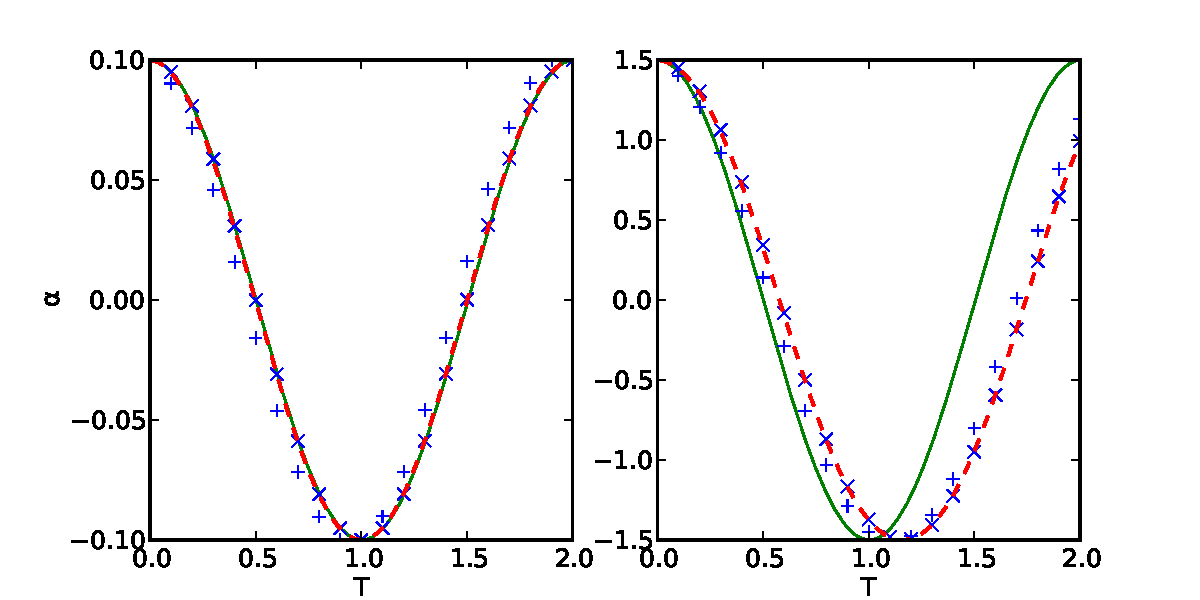
\includegraphics[width=\textwidth]{plots/pendel_loesung}
  \caption{Lösungen für ein Fadenpendel der Länge $l=1m$. Im linken Graphen
    ist die Ausgangslage $\alpha=1,5$, im rechten $\alpha=0,1$; in
    beiden Fällen ist die Ausgangsgeschwindigkeit 0. Die durchgezogene
  grüne Linie markiert die analytische Näherungslösung
  \eqref{eq:naeherung} für kleine Winkel. $\times$ markiert die
  Ergebnisse einer Integration mit dem einfachen Vorwärtsschritt
  \eqref{eq:simple} mit Zeitschritt $0,1s$, die gestrichelte rote
  Linie mit Zeitschritt $0,01s$. $+$ markiert die Lösung mit Hilfe des
  Velocity-Verlet-Algorithmus und Zeitschritt $0,1s$.}
  \label{fig:loesung}
\end{figure}

Für kleine Winkel gilt $\sin(\alpha)\approx\alpha$, und damit
\begin{equation}
  \ddot\alpha \approx = -\frac{g}{l}\alpha.
\end{equation}
Diese Differentialgleichung hat die allgemeine Lösung
\begin{equation}
  \alpha(t) = A \sin(\omega t + \phi)
  \label{eq:naeherung}
\end{equation}
mit $\omega=\sqrt{g/l}$, wie man sich leicht durch Einsetzen
überzeugt. Die Größen $A$ und $\phi$ ergeben sich aus den
Anfangsbedingungen, nämlich der Anfangsposition
\begin{equation}
  \alpha_0 = A \sin(\phi)
\end{equation}
und "~geschwindigkeit
\begin{equation}
  v_0 = A \omega \cos(\phi).
\end{equation}
Ist zum Beispiel $v_0=0$, so ist $\phi=\pi/2$ und $A=\alpha_0$, im
allgemeinen Fall ist
\begin{equation}
\phi =
\arctan\left(\frac{\alpha_0\omega}{v_0}\right)\quad\text{und}\quad
A = \frac{\alpha_0}{\sin(\phi)}.
\end{equation}
Wir haben nun eine geschlossene Lösung für die Position des Pendels,
so lange die Ausgangslage nicht zu sehr ausgelenkt ist. Um diese
Lösung zu visualisieren, nutzt man heute üblicherweise den Computer,
siehe Graph~\ref{fig:loesung}.

\subsection{Numerische Lösung}

Was passiert nun, wenn das System stärker ausgelenkt ist? Mit sehr
viel mehr Aufwand lässt sich auch für diesen Fall eine analytische
Lösung finden, allerdings in Form einer Reihe, die nicht mehr so
einfach zu zeichnen ist. Eine Alternative ist, die
Differentialgleichung \eqref{eq:pendelgln} mit Hilfe des Computers zu
berechnen. Wir sagen, wir "`simulieren"' das Pendel. Dazu fixieren wir
ein Einheitensystem, zum Beispiel eine Sekunde als Zeiteinheit und
einen Meter als Längeneinheit. In diesem System ist also $l=1$,
$g\approx 9,81$ und $\omega\approx 3,13$, falls des Pendel einen Meter
lang ist.

Zunächst müssen wir das Problem aber für den Computer anpassen, der ja
nur mit (endlich vielen) gewöhnlichen Zahlen rechnen kann, wir müssen
das Problem \emph{diskretisieren}. Wir betrachten nur die Zeitpunkte
\begin{equation}
  t_n = n\delta t, n=1(1)N,
\end{equation}
wobei der Zeitschritt $\delta t$ frei wählbar ist. Je kleiner $\delta
t$, desto genauer können wir $\alpha(t)$ bestimmen, allerdings steigt
natürlich die Anzahl der Schritte, die nötig sind, um eine feste
Gesamtzeit zu erreichen. Unsere Lösung, die Funktion $\alpha(t)$ wird
also durch ihre Werte $\alpha(t_n)$ an den diskreten Zeitpunkten
dargestellt.

\begin{figure}
  \centering
  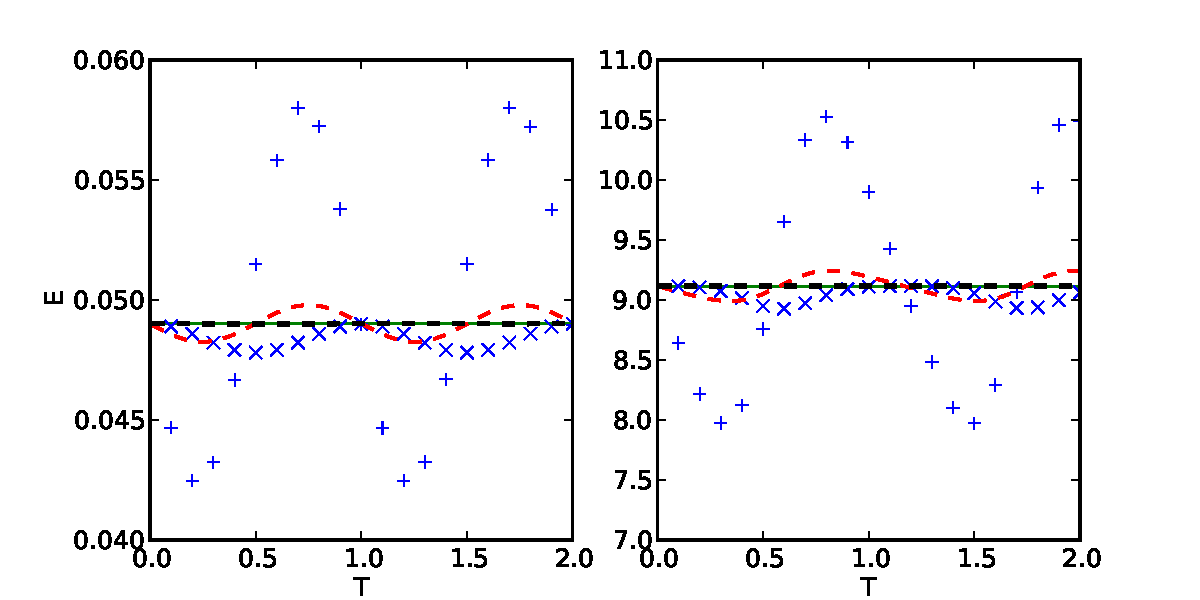
\includegraphics[width=\textwidth]{plots/pendel_energie}
  \caption{Energie als Funktion der Zeit, wieder für $l=1m$, und
    Ausgangslage $\alpha=1,5$ (links) und $\alpha=0,1$ (rechts) in
    Ruhe.  $+$ markiert die Ergebnisse einer Integration mit dem
    einfachen Vorwärtsschritt \eqref{eq:simple} mit Zeitschritt
    $0,1s$, die gestrichelte rote Linie mit Zeitschritt $0,01s$. $\times$
    markiert die Lösung mit Hilfe des Velocity-Verlet-Algorithmus und
    Zeitschritt $0,1s$, und die gestrichelte blaue Linie mit $0,01s$.}
  \label{fig:energie}
\end{figure}

Um Gleichung \eqref{eq:pendelgln} auf den Computer zu bringen, müssen
wir uns allerdings noch überlegen, wie wir mit der Ableitung verfahren.
Da wir die Ausgangsposition und "~ge\-schwin\-dig\-keit gegeben haben, liegt
es nahe, die Gleichung zu integrieren:
\begin{equation}
  v(t+\delta t) = \dot\alpha(t + \delta t) = v(t) + \int_{t}^{t+\delta t}
  -\omega^2\sin \alpha(\tau)\, d\tau.
\end{equation}
Da $\delta t$ aber unser Zeitschritt ist, wir also nichts weiter über
$\alpha(\tau)$ wissen, bietet sich die folgende Näherung an:
\begin{equation}
  v(t+\delta t) \approx v(t) - \omega^2\sin\alpha(t) \delta t.
\end{equation}
Analog ergibt sich dann durch nochmalige Integration:
\begin{equation}
  \alpha(t+\delta t) \approx \alpha(t) + v(t) \delta t.
  \label{eq:simple}
\end{equation}
Ausgehend von
\begin{equation}
  \alpha(0) = \alpha_0 \quad\text{und}\quad v(0) = v_0
\end{equation}
lässt sich damit also $\alpha(t)$ numerisch bestimmen. Der
Quellcode~\ref{lst:pendel} zeigt, wie eine einfach Implementation in
Python aussehen könnte.

Wie kann man nun überprüfen, ob diese Lösung tatsächlich korrekt ist?
Da das System abgeschlossen ist, muss seine Energie
\begin{equation}
  E = \frac{1}{2} l^2 v(t)^2 + gl (1 - \cos(\alpha(t)))
\end{equation}
erhalten sein. Lässt man sich diese allerdings ausgeben, stellt man
fest, dass $E(t)$ erheblich schwankt, vergleiche
Graph~\ref{fig:energie}. Dies lässt sich durch Verringern des
Zeitschritts beheben, das kostet aber entsprechend mehr Rechenzeit.

Eine bessere Alternative ist, den Algorithmus zu verbessern, was
wiederum etwas analytische Arbeit erfordert. Wir betrachten die
Taylorentwicklungen
\begin{align}
  \alpha\left(t+\delta t\right) &= \alpha\left(t+\frac{\delta t}{2}\right) + \frac{\delta t}{2}
  v\left(t+\frac{\delta t}{2}\right) + \frac{\delta t^2}{8} F\left(t+\frac{\delta t}{2}\right) + \O(\delta t^3)
  \intertext{und}
  \alpha\left(t\right) &= \alpha\left(t+\frac{\delta t}{2}\right) - \frac{\delta t}{2}
  v\left(t+\frac{\delta t}{2}\right) + \frac{\delta t^2}{8} F\left(t+\frac{\delta t}{2}\right) - \O(\delta t^3).
\end{align}
Durch Subtraktion ergibt sich
\begin{align}
  \alpha(t+\delta t) = \alpha(t) + \delta t\,v\left(t+\frac{\delta t}{2}\right) + \O(\delta t^4).
\end{align}
Die Geschwindigkeiten an den halben Zeitschritten erhält man einfach
durch $v(t + \delta t /2) = v(t) + \delta t F(t) / 2$.
Zusammengefasst ergibt sich der folgende \emph{Velocity-Verlet-Algorithmus}:
\begin{align}
  v\left(t + \frac{\delta t}{2}\right) &= v(t) + \frac{\delta t}{2} F(t) \\
  \alpha(t + \delta t) &= \alpha(t) + v\left(t + \frac{\delta t}{2}\right) \\
  v(t + \delta t) &= v\left(t + \frac{\delta t}{2}\right) + \frac{\delta t}{2}
  F(t + \delta t),
\end{align}
der anders als die direkte Vorgehensweise vorher numerisch stabil ist
und quasi keine Energieschwankungen aufzeigt, vergleiche
Graph~\ref{fig:energie}. 
Im Quellcode~\ref{lst:pendel} ist alternativ auch dieser Integrator
implementiert. Obwohl er nur unwesentlich komplizierter ist als der
einfache Integrator zuvor, erreicht etwa dieselbe Genauigkeit wie
dieser mit einem Zehntel der Zeitschritte.

Als weiterer Test bietet sich an, bei kleinen Auslenkungen mit der
analytisch bekannten Lösung zu vergleichen, die gut reproduziert wird,
siehe Graph~\ref{fig:loesung}. Bei größeren Anfangsauslenkungen oder
-ge\-schwin\-dig\-keiten ist die Abweichung allerdings sehr groß, weil
hier die analytische Näherung versagt. Im Rahmen ihrer Genauigkeit
erlaubt also die numerische Lösung, das vorgegebene Modell in einem
größeren Parameterraum auf sein Verhalten hin zu untersuchen, als
analytisch möglich wäre.

\lstinputlisting[style=floating,firstline=10,
caption={[Fadenpendel] Python-Code zum Fadenpendel
  mit graphisch aufbereiteter Ausgabe mit Hilfe der \texttt{matplotlib}.},
label=lst:pendel]{pendel.py}

%%% Local Variables: 
%%% mode: latex
%%% TeX-master: "padc"
%%% TeX-PDF-mode: t
%%% End: 

% Dies ist Teil der Vorlesung Physik auf dem Computer, SS 2012,
% Axel Arnold, Universitaet Stuttgart.
% 
% Dieses Werk ist unter einer Creative Commons-Lizenz vom Typ
% Namensnennung-Weitergabe unter gleichen Bedingungen 3.0 Deutschland
% zugänglich. Um eine Kopie dieser Lizenz einzusehen, konsultieren Sie
% http://creativecommons.org/licenses/by-sa/3.0/de/ oder wenden Sie sich
% schriftlich an Creative Commons, 444 Castro Street, Suite 900, Mountain
% View, California, 94041, USA.
\chapter{Lineare Algebra \textrm{I}}
\index{Gleichungssysteme>lineare}

Lineare Gleichungssysteme sind die einfachste Art von
Gleichungssystemen, für die sich zum Beispiel leicht bestimmen lässt,
ob und wieviele Lösungen es gibt. Daher führt man auch die Lösung
komplexerer Probleme, wie zum Beispiel Differentialgleichungen, oft
auf die Lösung eines Satzes von linearen Gleichungssystemen
zurück. Lineare Gleichungssysteme sind in diesem Sinne eine der
wesentlichen Grundlagen der numerischen Mathematik. Der händischen
Lösung der Systeme steht dabei vor allem ihre Größe im Weg ---
Finite-Elemente-Rechnungen können leicht die Lösung von
Gleichungssystemen mit Millionen von Variablen erfordern. Mit modernen
Algorithmen und Computern lassen sich solche Gleichungssysteme
allerdings schnell und zuverlässig lösen. In diesem Kapitel lernen wir
die grundlegende Methode zum Lösen von Gleichungssystemen kennen,
nämlich die allgemeine, aber langsame Gaußelimination. Daneben lernen
wir noch die LU-Zerlegung und die Choleskyzerlegung kennen, die mit
etwas Vorarbeit eine effizientere Lösung erlauben und im folgenden oft
zum Einsatz kommen werden.

Wir betrachten also folgendes Problem: Sei $A=(a_{ik})\in\RR^{m\times
  n}$, $b\in\RR^m$. Gesucht ist die Lösung $x\in\RR^n$ des
Gleichungssystems
\begin{equation}
  \label{eq:lgs}
  \begin{matrix}
    a_{11}x_1 &+&  a_{12}x_2 &+& \ldots &+& a_{1n}x_n &=& b_1\\
    a_{21}x_1 &+&  a_{22}x_2 &+& \ldots &+& a_{2n}x_n &=& b_2\\
    \vdots   &&   \vdots   &&         && \vdots  && \vdots\\
    a_{m1}x_1 &+&  a_{m2}x_2 &+& \ldots &+& a_{mn}x_n &=& b_m
  \end{matrix}
\end{equation}
oder kurz $Ax=b$. In dieser allgemeinen Form ist weder garantiert,
dass es eine Lösung gibt (z.B. $A=0$, $b\neq 0$), noch, dass diese
eindeutig ist ($A=0$, $b=0$).

\section{\keyword{Dreiecksmatrizen}}

Eine Matrix $A\in\RR^{n\times n}$ heißt eine \emph{rechte obere
  Dreiecksmatrix}, wenn sie quadratisch ist und $a_{ij}=0$ für $i>j$.
Analog kann man auch die linken unteren Dreiecksmatrizen definieren,
mit $a_{ij}=0$ für $i<j$. In jedem Fall bilden rechte obere und linke
untere Dreiecksmatrizen jeweils Unteralgebren der Matrixalgebra, d.h.,
sie sind abgeschlossen unter Addition und Multiplikation. Die
Schnittmenge dieser Algebren ist wiederum die Algebra der
\emph{\keyword{Diagonalmatrizen}}.

Ist $A$ eine rechte obere Dreiecksmatrix, so hat das Gleichungssystem
die Form
\begin{equation}
  \begin{matrix}
    a_{11}x_1 &+&  a_{12}x_2 &+& \ldots &+& a_{1n}x_n &=& b_1\\
             &&  a_{22}x_2 &+& \ldots &+& a_{2n}x_n &=& b_2\\
             &&            && \ddots && \vdots  && \vdots\\
             &&            &&        && a_{nn}x_n &=& b_n.
  \end{matrix}
\end{equation}
Dieses Gleichungssystem hat genau dann eine Lösung, wenn $A$ regulär
ist, also $\det A=\prod_{i=1}^na_{ii}\neq 0$. Die Lösung kann dann durch
\emph{Rücksubstitution} direkt bestimmt werden:
\begin{equation}
  \label{eq:ruecksubst}
  x_i = \frac{1}{a_{ii}}\left( b_i - \sum_{k=i+1}^n a_{ik}x_k\right)
  \quad\text{für}\; i=n(-1)1.
\end{equation}

Für reguläre \emph{linke untere Dreiecksmatrizen} ergibt sich die
Lösung entsprechend durch \emph{Vorwärtssubstitution}:
\begin{equation}
  \label{eq:vorwsubst}
  x_i = \frac{1}{a_{ii}}\left( b_i - \sum_{k=1}^{i-1} a_{ik}x_k\right)
  \quad\text{für}\; i=1(1)n.
\end{equation}

Für Diagonalmatrizen ist die Situation natürlich einfacher, es gilt
\begin{equation}
  x_i = \frac{1}{a_{ii}} b_i
  \quad\text{für}\; i=1(1)n.
\end{equation}

\begin{sloppypar}
  SciPy stellt für Dreiecksmatrizen spezielle Löserroutinen zur
  Verfügung, \scipy{scipy.linalg.solve_triangular(A, b, lower=False)},
  wobei \argd{lower} angibt, ob  \argd{A} eine linke untere statt rechte
  obere Dreiecksmatrix ist.
\end{sloppypar}

\section{\keyword{Gaußelimination}}

Die Gaußelimination ist ein Verfahren, um eine beliebiges
Gleichungssystem $Ax=b$, mit $A\in\RR^{m\times n}$, auf die
äquivalente Form
\begin{equation}
  \label{eq:rform}
  \begin{pmatrix}
    R & K \\
    0 & 0
  \end{pmatrix} x' = b'
\end{equation}
zu bringen, wobei $R$ eine reguläre rechte obere Dreiecksmatrix und
$K\in\RR^{k\times l}$ beliebig ist, und $x'$ eine Permutation
(Umordnung) von $x$. Dieses Gleichungssystem hat offenbar nur dann
eine Lösung, wenn $b_i'=0$ für $i=m-k+1(1)m$.

Diese ist im allgemeinen auch nicht eindeutig, vielmehr können die
freien Variablen $x_\text{K} = (x'_i)_{i=n-k+1}^{n}$ frei gewählt
werden. Ist $x_\text{R} = (x'_i)_{i=1}^{n-k}$ der Satz der
verbleibenden Lösungsvariablen, so gilt also
\begin{equation*}
  x_\text{L} = R^{-1}b' - R^{-1}K x_\text{K}.
\end{equation*}
Die Lösungen ergeben sich daraus als
\begin{equation}
  x' =
  \begin{pmatrix}
    R^{-1}b'\\
    0
  \end{pmatrix} +
  \left<
    \begin{pmatrix}
      -R^{-1}K_i\\
      e_i
    \end{pmatrix}
  \right>,
\end{equation}
wobei $K_i$ die $i$-te Spalte von K und
$\left<\right>$ den aufgespannten Vektorraum bezeichnet. Die
Ausdrücke, die $R^{-1}$ enthalten, können durch Rücksubstitution bestimmt
werden.

Um das System $Ax=b$, das wir im folgenden als $A|b$ zusammenfassen,
auf diese Form zu bringen, stehen folgende Elementaroperationen zur
Verfügung, die offensichtlich die Lösung nicht verändern:
\begin{enumerate}
\item Vertauschen zweier Gleichungen (Zeilentausch in $A|b$)
\item Vertauschen zweier Spalten in $x$ und $A$ (Variablenaustausch)
\item Addieren eines Vielfachen einer Zeile zu einer anderen
\item Multiplikation einer Zeile mit einer Konstanten ungleich 0
\end{enumerate}
Die Gausselimination nutzt nun diese Operationen, um die Matrix
spaltenweise auf die gewünschte Dreiecksform zu bringen. Dazu werden
Vielfache der ersten Zeile von allen anderen abgezogen, so dass die
Gleichung die Form
\begin{equation}
  \left(\begin{array}{lll|c}
      a_{11}^{(0)} & a_{12}^{(0)}\ldots &a_{1n}^{(0)} & b_1^{(0)}\\
      0     & a_{22}^{(1)}\ldots &a_{2n}^{(1)} & b_2^{(1)}\\
      \vdots& \vdots      &\vdots& \vdots\\
      0     & a_{m2}^{(1)}\ldots &a_{mn}^{(1)} & b_m^{(1)}\\
    \end{array}\right) =: A^{(1)} | b^{(1)}
\end{equation}
annimmt, wobei
\begin{equation}
  \begin{array}{rcll}
    a_{ik}^{(1)} &=& a_{ik}^{(0)} -  l_{i}^{(1)}a_{1k}^{(0)}
    & \quad\text{für}\; i=2(1)n, k=1(1)m\\[0.3em]
    b_{i}^{(1)} &=& b_{i}^{(0)} - l_{i}^{(1)} b_{1}^{(0)}
    & \quad\text{für}\; i=2(1)n \\[0.3em]
    a_{1k}^{(1)} &=& a_{1k}^{(0)},\quad b_{1}^{(1)} = b_{1}^{(0)}
    & \quad\text{sonst}
  \end{array}
  \quad\text{mit}\, l_{i}^{(1)} = \frac{a_{i1}^{(0)}}{a_{11}^{(0)}}.
\end{equation}
Mit dem verbleibenden Resttableau wird nun
genauso weiter verfahren:
\begin{equation}
  \label{eq:gausseli}
  \begin{array}{rcll}
    a_{ik}^{(r)} &=& a_{ik}^{(r-1)} -  l_{i}^{(r)}a_{r,k}^{(r-1)}
    & \quad\text{für}\; i=r+1(1)n, k=r(1)m\\[0.3em]
    b_{i}^{(r)} &=& b_{i}^{(r-1)} - l_{i}^{(r)} b_{r}^{(r-1)}
    & \quad\text{für}\; i=r+1(1)n \\[0.3em]
    a_{ik}^{(r)} &=& a_{ik}^{(r-1)},\quad b_{i}^{(r)} = b_{i}^{(r-1)}
    & \quad\text{sonst}
  \end{array}
  \text{mit}\, l_{i}^{(r)} = \frac{a_{ir}^{(r-1)}}{a_{rr}^{(r-1)}}.
\end{equation}
Das Verfahren ist beendet, wenn das Resttableau nur noch eine Zeile hat.

Ist während eines Schrittes $a_{rr}^{(r-1)} = 0$ und
\begin{enumerate}
\item nicht alle $a_{ir}^{(r-1)}=0$, $i=r+1(1)m$. Dann tauscht man
  Zeile $r$ gegen eine Zeile $i$ mit $a_{ir}^{(r-1)}\neq 0$, und fährt
  fort.
\item alle $a_{ir}^{(r-1)}=0$, $i=r(1)m$, aber es gibt ein
  $a_{ik}^{(r-1)}\neq 0$ mit $i,k\ge r$. Dann vertauscht man zunächst
  Zeile $r$ mit Zeile $i$, tauscht anschließend Spalte $k$ mit
  Spalte $r$, und fährt fort.
\item alle $a_{ik}^{(r-1)}=0$ für $i,k \ge r$. Dann hat
  $A^{(r-1)}|b^{(r-1)}$ die gewünschte Form \eqref{eq:rform} erreicht,
  und das Verfahren terminiert.
\end{enumerate}

Das Element $a_{rr}^{(r-1)}$ heißt auch \emph{Pivotelement}, da es
sozusagen der Dreh- und Angelpunkt des iterativen Verfahrens ist.  In
der Praxis ist es numerisch günstiger, wenn dieses Element möglichst
groß ist. Das lässt sich erreichen, in dem wie in den singulären
Fällen verfahren wird, also Zeilen oder Spalten getauscht werden, um
das betragsmäßig maximale $a_{ik}^{(r-1)}$ nach vorne zu
bringen. Folgende Verfahren werden unterschieden
\begin{itemize}
\item \emph{kanonische \keyword{Pivotwahl}}: es wird stets
  $a_{rr}^{(r-1)}$ gewählt und abgebrochen, falls dieses betragsmäßig
  zu klein wird. Diese Verfahren scheitert schon bei einfachen
  Matrizen (z.B. {\tiny $\begin{pmatrix} 0 & 1\\ 1 &
      0\end{pmatrix}$}), und kann daher nur eingesetzt werden, wenn
  die Struktur der Matrix sicherstellt, das $a_{rr}^{(r-1)}$ stets
  hinreichend groß ist.
\item \emph{Spaltenpivotwahl}: es wird wie oben im 1. Fall nur in der
  Spalte maximiert, d.h. wir wählen als  Pivotelement
  \begin{equation}
    i_0 = \text{argmax}_{i>r} \lvert a_{ir}^{(r-1)}\rvert
  \end{equation}
  und tauschen Zeilen $i_0$ und $r$; die Variablenreihenfolge bleibt
  unverändert. Ist die Matrix $A$ quadratisch, bricht das Verfahren
  genau dann ab, wenn $A$ singulär ist.
\item \emph{Totalpivotwahl}: wie oben im 2. Fall wird stets das maximale
  Matrixelement im gesamten Resttableau gensucht, also
  \begin{equation}
    i_0,k_0 = \text{argmax}_{i,k>r} \lvert a_{ik}^{(r-1)}\rvert.
  \end{equation}
  Dann vertauscht man zunächst Zeile $r$ mit Zeile $i_0$, und tauscht
  anschließend Spalte $k_0$ mit Spalte $r$, wobei man sich noch die
  Permutation der Variablen geeignet merken muss, zum Beispiel als
  Vektor von Indizes.
\end{itemize}

Unabhängig von der Pivotwahl benötigt die Gaußelimination bei
quadratischen Matrizen im wesentlichen $\O(n^3)$
Fließkommaoperationen. Das ist relativ langsam, daher werden wir
später bessere approximative Verfahren kennenlernen. Für Matrizen
bestimmter Struktur, zum Beispiel Bandmatrizen, ist die
Gaußelimination aber gut geeignet. NumPy bzw. SciPy stellen daher auch
keine Gaußelimination direkt zur Verfügung.
\scipy{scipy.linalg.solve(A, b)} ist ein Löser für Gleichungssysteme
$Ax=b$, der immerhin auf der LU-Zerlegung durch Gaußelimination
basiert. Dieser Löser setzt allerdings voraus, dass die Matrix nicht
singulär ist, also eindeutig lösbar.
 
\section{\keyword{Matrixinversion}}

Ist $A\in\RR^{n\times n}$ regulär, so liefert die Rücksubstitution
implizit die Inverse von $A$, da für beliebige $b$ das
Gleichungssystem $Ax=b$ gelöst werden kann. Allerdings muss das für
jedes $b$ von neuem geschehen. Alternativ kann mit Hilfe der
Gaußelimination auch die Inverse von $A$ bestimmt werden. Dazu wird
das Tableau $A|I$ in das Tableau $I|A^{-1}$ transformiert, wobei $I$
die $n\times n$-Einheitsmatrix bezeichnet. Die Vorgehensweise
entspricht zunächst der Gaußelimination mit
Spaltenpivotwahl. Allerdings werden nicht nur die Elemente unterhalb
der Diagonalen, sondern auch oberhalb eliminiert. Zusätzlich wird die
Pivotzeile noch mit $1/a_{ii}^{(i-1)}$ multipliziert, so dass das $A$
schrittweise die Form
\begin{equation}
  \left(\begin{array}{cccc}
      1     & 0      & a_{12}^{(2)}\ldots &a_{1n}^{(2)} \\
      0     & 1      & a_{22}^{(2)}\ldots &a_{2n}^{(2)} \\
      \vdots& 0      & a_{32}^{(2)}\ldots &a_{3n}^{(2)} \\
      \vdots& \vdots & \vdots             & \vdots      \\
      0     & 0      & a_{n2}^{(2)}\ldots &a_{nn}^{(2)} \\
    \end{array}\right)
\end{equation}
annimmt. Das Verfahren ist allerdings numerisch nicht sehr stabil, und
generell sollte die explizite Berechnung der Inversen wann inner
möglich vermieden werden. SciPy stellt die Matrixinversion als
Funktion \scipy{scipy.linalg.inv(A)} zur Verfügung.

Eine Ausnahme bilden Matrizen der Form $I + A$ mit $\lVert A \rVert =
\max \lVert Ax\rVert / \lVert x \rVert < 1$. Dann ist
\begin{equation}
  (I+A)^{-1} = I - A + A^2 - A^3 + \cdots
\end{equation}
eine gut konvergierende Näherung der Inversen.

\section{\keyword{LU-Zerlegung}}
\index{LR-Zerlegung}

Eine weitere Anwendung der Gaußelimination ist die LU-Zerlegung von
bestimmten quadratischen Matrizen. Dabei wird eine Matrix
$A\in\RR^{n\times n}$ so in eine ein linke untere Dreiecksmatrix $L$
und eine rechte obere Dreiecksmatrix $U$ zerlegt, dass $A=L\cdot U$.
Um die LU-Zerlegung eindeutig zu machen, vereinbart man üblicherweise,
dass $l_{ii}=1$ für $i=1(1)n$. Das $U$ steht übrigens für das
englische "`upper right"' und $L$ für "`lower left"'. Im Deutschen
findet sich vereinzelt noch der Begriff LR-Zerlegung, wobei hier L für
eine linke untere und R für eine rechte obere Matrix steht.

Ist eine solche Zerlegung einmal gefunden, lässt sich das
Gleichungssystem $Ax=b$ für beliebige $b$ effizient durch Vorwärts-
und Rücksubstitution lösen:
\begin{equation}
  L y = b,\, U x = y \quad\implies\quad Ax = L\,U x = L y = b.
\end{equation}
Zunächst wird also $y$ durch Vorwärtssubstitution berechnet,
anschließend $x$ durch Rückwärtssubstitution. Die Inverse lässt
sich so auch bestimmen:
\begin{equation}
  L y_i = e_i,\, U x_i = y_i\quad\text{für}\; i=1(1)n
  \quad\implies\quad  A^{-1} = \left(x_1,
    \ldots, x_n\right).
\end{equation}
Die Determinante von $A=L\cdot U$ ist ebenfalls einfach zu bestimmen:
\begin{equation}
  \det A = \det L\,\det U = \prod_{i=1}^n u_{ii}
\end{equation}

Um die LU-Zerlegung zu berechnen, nutzen wir wieder die
Gaußelimination.  Kann bei $A\in\RR^{n\times n}$ die Gaußelimination
in kanonischer Pivotwahl durchgeführt werden, so ist die LU-Zerlegung
von $A$ durch $U=A^{(n-1)}$, also die finale, auf rechte obere
Dreiecksform transformierte Matrix, und durch die Matrix
\begin{equation}
  L =
  \begin{pmatrix}
    1       &          &         &          & 0 \\
    l_1^{(0)} & 1       &         &           &  \\
    l_2^{(0)} & l_2^{(1)} & 1       &          &  \\
    \vdots  &          & \ddots & \ddots    & \\
    l_n^{(0)} & \ldots  & \ldots  & l_n^{(n-1)} & 1
  \end{pmatrix}
\end{equation}
der Updatekoeffizienten aus \eqref{eq:gausseli} gegeben.

Wie bereits gesagt, ist die Voraussetzung, dass die Gaußelimination
mit kanonischer Pivotwahl durchgeführt werden kann, stark, und
schließt selbst einfache Matrizen wie {\tiny $\begin{pmatrix} 0 & 1\\
    1 & 0\end{pmatrix}$} aus. Wie man sich leicht überlegt, besitzt
diese Matrix allerdings keine LU-Zerlegung.

Für manche Anwendungen ist es günstiger, wenn $L$ und $U$ normiert
sind. Dann benutzt man die \keyword{LDU-Zerlegung} $A=LDU$, mit $L$
linker unterer Dreiecksmatrix, $D$ Diagonalmatrix und $U$ rechter
oberer Dreiecksmatrix. Jetzt müssen $l_{ii}=1$ und $r_{ii}=1$
sein. Die LDU-Zerlegung ergibt sich aus der LU-Zerlegung durch $d_{ii}
= u_{ii}$ und $u'_{ik}=u_{ik}/u_{ii}$.

In SciPy ist die LU-Zerlegung in den Funktionen
\scipy{scipy.linalg.lu_factor(A)} oder \scipy{scipy.linalg.lu(A)} (zur
Zerlegung der Matrix A) und \scipy{scipy.linalg.lu_solve((lu,piv), b)}
(zum Lösen des LGS) implementiert.

\section{Cholesky-Zerlegung}
\index{Cholesky>-Zerlegung}

Wir betrachten im folgenden nur symmetrische, positiv definite
Matrizen, wie sie gerade in der Physik oft vorkommen. Auch in der
Optimierung spielen diese eine wichtige Rolle. Sei $A=LDU$ eine
LDU-Zerlegung einer symmetrischen Matrix, dann gilt
\begin{equation}
  LDU = A = A^T = (LDU)^T = U^T D L^T.
\end{equation}
Da die LDU-Zerlegung aber eindeutig ist und $U^T$ eine normierte,
linke untere Dreiecksmatrix und $L^T$ eine normierte, rechte obere
Dreiecksmatrix, so gilt $U=U^T$, und damit
\begin{equation}
  A = U^TDU = \widehat{U}^T\widehat{U} \quad\text{mit}\; \widehat{U}=\text{diag}(\sqrt{d_{ii}})U.
\end{equation}
Dies ist die Cholesky-Zerlegung. Anstatt die Gaußelimination
durchzuführen, lässt sich die Zerlegung aber auch direkt mit Hilfe des
\emph{Cholesky-Verfahrens}\index{Cholesky>-Verfahren} bestimmen: Sei
$A=\widehat{R}^T\widehat{R}$ eine Cholesky-Zerlegung.
Da $\widehat{R}$ unterhalb der Diagonalen nur 0 enthält, gilt
\begin{equation}
  a_{ik} = \sum_{l=1}^{i} \hat{r}_{li}\hat{r}_{lk} \quad\text{für}\;
  i=1(1)n,\,k=1(1)n.
\end{equation}
Daraus lässt sich die erste Zeile von $\widehat{R}$ direkt ablesen:
\begin{equation}
\hat{r}_{11} = \sqrt{a_{11}}\quad\text{und}\;
\hat{r}_{1k} = \frac{a_{1k}}{\hat{r}_{11}} \quad\text{für}\;k=2(1)n.
\end{equation}
Die nächsten Zeilen lassen sich analog bestimmen, da für jedes $i$
\begin{equation}
  a_{ii} = \sum_{l=1}^{i} \hat{r}_{li}^2\quad\implies\;
  \hat{r}_{ii} = \sqrt{a_{ii} - \sum_{l=1}^{i-1} \hat{r}_{li}^2}.
\end{equation}
Für die restlichen Elemente der Zeile gilt
\begin{equation}
  \hat{r}_{ik} = \frac{1}{\hat{r}_{ii}}\left(a_{ik} - \sum_{l=1}^{i-1}\hat{r}_{li}\hat{r}_{lk}\right) \quad\text{für}\;k=i+1(1)n
\end{equation}
Das Cholesky-Verfahren ist wie die Gaußelimination von der Ordnung
$\O(n^3)$, braucht aber nur halb so viele Operationen. In SciPy ist die
Cholesky-Zerlegung als \scipy{scipy.linalg.cholesky(A)} implementiert.

\section{\keyword{Bandmatrizen}}

Im folgenden werden wir oft mit $k$-Bandmatrizen zu tun haben, also
Matrizen, bei denen nur die Diagonale und einige Nebendiagonalen
besetzt sind. Diagonalmatrizen sind also 1-Bandmatrizen, eine
\emph{Dreibandmatrix}\index{Dreibandmatrizen} hat die Form
\begin{equation}
  \begin{pmatrix}
    d_1 & t_1    &     & & 0 \\
    b_1 & d_2    & t_2 \\
    {}  & \ddots & \ddots & \ddots \\
    {}  &        & b_{n-2} & d_{n-1} & t_{n-1}\\
    0   &        &        & b_{n-1} & d_n
  \end{pmatrix}.
\end{equation}
Für Matrizen dieser Form ist die Gaußelimination mit kanonischer
Pivotwahl sehr effizient, da pro Iteration jeweils nur die erste Zeile
des Resttableaus verändert werden muss. Dadurch ist der Rechenaufwand
nur noch linear in der Matrixgröße bzw. Länge der Bänder. Die
Dreiecksmatrizen $L$ und $U$ der LU-Zerlegung sind zusätzlich
(Drei-) Bandmatrizen, wobei $L$ nur auf der Haupt und der unteren
Nebendiagonalen von Null verschiedene Einträge hat, $U$ nur auf der
Diagonalen und der Nebendiagonalen oberhalb.

SciPy stellt für Bandmatrizen ebenfalls spezielle Löserroutinen zur
Verfügung, \scipy{scipy.linalg.solve_banded((l,u), A, b)},
wobei \argd{l} und \argd{u} die Anzahl der Nebendiagonalen oberhalb
und unterhalb angeben, und \argd{A} die Matrix in Bandform
angibt.

%%% Local Variables: 
%%% mode: latex
%%% TeX-master: "padc"
%%% TeX-PDF-mode: t
%%% End: 

% Dies ist Teil der Vorlesung Physik auf dem Computer, SS 2012,
% Axel Arnold, Universitaet Stuttgart.
% 
% Dieses Werk ist unter einer Creative Commons-Lizenz vom Typ
% Namensnennung-Weitergabe unter gleichen Bedingungen 3.0 Deutschland
% zugänglich. Um eine Kopie dieser Lizenz einzusehen, konsultieren Sie
% http://creativecommons.org/licenses/by-sa/3.0/de/ oder wenden Sie sich
% schriftlich an Creative Commons, 444 Castro Street, Suite 900, Mountain
% View, California, 94041, USA.

\chapter{Darstellung von Funktionen}

Auch moderne Prozessoren beherrschen nur die Grundrechenarten. Wie
kann man also auf einem Computer kompliziertere Funktionen berechnen,
wie z.B. die Sinusfunktion?

Beispielsweise könnte man die Funktionen als Vektor von
Funktionswerten speichern. Für die graphische Darstellung reicht das
aus, aber um Funktionen mit wenigstens sechs Stellen Genauigkeit im
Computer bereitzustellen, wären Millionen von Stützstellen nötig.

Daher müssen bessere Darstellungen für Funktionen genutzt werden.  Um
beliebige Funktionen auf dem Computer berechnen zu können, führt man
diese meist auf (stückweise definierte) Polynome zurück, die nur mit
Hilfe der Grundrechenarten berechnet werden können. Dies ist selbst
dann der Fall, wenn ein Prozessor gewisse Funktionen scheinbar in
Hardware implementiert hat; tatsächlich führt dieser intern die
notwendigen elementaren Operationen durch.

\section{\keyword{Horner-Schema}}
\label{sec:horner}

Die naive Auswertung eines Polynoms $\sum_{i=0}^{n} c_ix^{i}$ mit
$n+1$ Termen bzw.\ vom Grad $n$ benötigt $n$ Additionen und $2n$
Multiplikationen sowie einen Zwischenspeicher für die Potenzen $x^i$
des Arguments $x$. Besser ist die Auswertung des Polynoms nach dem
Horner-Schema:
\begin{equation}
  \label{eq:horner}
  \sum_{i=0}^{n} c_ix^{i} = c_0 + x(c_1 + x(c_2 + x(\ldots (c_{n-1} + x c_{n})))).
\end{equation}
Wird dieser Ausdruck von rechts nach links ausgewertet, so muss das
Ergebnis in jedem Schritt nur mit $x$ multipliziert und der nächste
Koeffizient addiert werden, was nur $n$ Multiplikationen und
Additionen benötigt. Auch muss kein Zwischenwert gespeichert werden,
was Prozessorregister spart. Als C-Code sieht die Auswertung des
Hornerschemas so aus:
\begin{lstlisting}[language=C]
double horner(double *series, int n, double x)
{
    double r = series[n];
    for(int i = n-1; i >= 0; --i)
        r = r*x + series[i];
    return r;
}
\end{lstlisting}
\sloppypar Die Polynomauswertung stellt NumPy als
\scipy{numpy.polyval(x, c)} zur Verfügung. \argd{c} bezeichnet die
Koeffizienten des Polynoms und \argd{x} das Argument, für das das
Polynom ausgewertet werden soll.

Eine weitere Anwendung des Hornerschemas ist die Polynomdivision durch
lineare Polynome der Form $x-x_0$, die zum Beispiel wichtig für die
iterative Bestimmung von Nullstellen ist. Es gilt nämlich
\begin{equation}
  \label{eq:polynomdiv}
  P(x) = \sum_{i=0}^{n} c_ix^{i} = 
  \left(\sum_{i=0}^{n-1} d_{i+1}x^{i}\right)(x-x_0) + d_0,
\end{equation}
wobei $d_i = c_i + x_0(c_{i+1} + x_0(\ldots (c_{n-1} + x_o c_n)))$ die
Zwischenterme des Hornerschemas bei Auswertung an der Stelle $x_0$
sind. $d_0$ ist dabei der Divisionsrest; ist $P(x)$ durch $x-x_0$
teilbar, so ist $d_0=0$. 

Dies zeigt man durch Induktion: für $P(x) = c_1 x + c_0$ ist offenbar
$P(x) = c_1(x-x_0) + c_0 + x c_1 = d_1(x-x_0) + d_0$. Für Grad $n$ ist
also
\begin{equation}
    P(x) = x \left(\sum_{i=0}^{n-1} c_{i+1}x^{i}\right) + c_0
    = x\left(\sum_{i=0}^{n-2} d'_{i+1}x^{i}(x-x_0) + d'_0\right) +
    d_0
\end{equation}
wobei sich die $d'_i = c_{i+1} + x_0(c_{i+2} + x_0(\ldots (c_{n-1} +
x_o c_n))) = d_{i+1}$ bei der Polynomdivision von $\sum_{i=0}^{n-1}
c_{i+1}x^{i}$ durch $x-x_0$ ergeben. Daher ist
\begin{equation}
    P(x) = \left(\sum_{i=0}^{n-2} d_{i+2}x^{i+1} + d_1\right)(x-x_0) +
    d_0 + x_0 d_1,
\end{equation}
was zu zeigen war.

\section{Taylorreihen}
\index{Taylorreihe}

\begin{figure}
  \centering
  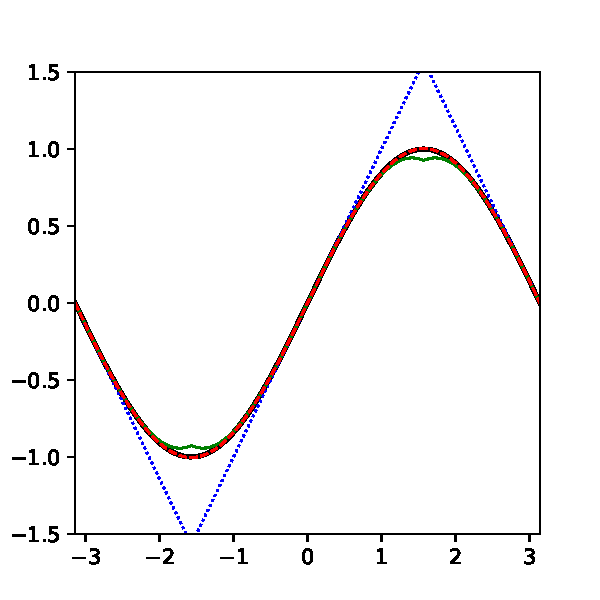
\includegraphics[width=0.5\textwidth]{plots/sinus}
  \caption{Näherung der Sinusfunktion durch die abgeschnittene
    Taylorreihe. Als schwarze durchgezogene Linie ist die tatsächliche
    Sinusfunktion dargestellt, blau gepunktet ist die Näherung erster
    Ordnung um Null, $x$, grün durchgezogen ist die kubische Näherung
    $x - x^3/6$, und rot gestrichelt $x-x^3/6 + x^5/120$. Die Kurven
    nutzen die Symmetrie der Sinuskurve, sind also an $\pm\pi/2$
    gespiegelt.}
  \label{fig:sinus}
\end{figure}

Nachdem wir nun wissen, wie Polynome effizient ausgewertet werden
können, stellt sich die Frage, wie man ein gutes Näherungspolynom für
eine Funktion bekommt. Dazu gibt es viele verschiedene Ansätze, deren
Vor- und Nachteile im Folgenden kurz besprochen werden. Der älteste
Ansatz, der auch in der Analytik weiten Einsatz findet, ist die
Taylorentwicklung.  Ist eine Funktion $f$ um einen Punkt $x_o$
hinreichend gut differenzierbar, lässt sie sich als bekannterweise
lokal als Taylorreihe darstellen:
\begin{equation}
  f(x) = \sum_{i=0}^\infty \frac{f^{(i)}(x_0)}{i!} (x-x_0)^i,
  \label{eq:taylor}
\end{equation}
wobei $f^{(i)}(x)$ die $i$-te Ableitung von $f$ an der Stelle $x$
bezeichnet.  Falls die Ableitungen existieren und $x-x_0$ klein genug
ist, so konvergiert diese Darstellung schnell, und einige Terme
genügen, um zufriedenstellende Genauigkeit zu erreichen. Lokal um den
Entwicklungspunkt $x_0$ is eine abgeschnittene Taylorreihe also eine
gute polynomielle Näherung. Leider gibt es für die meisten Funktionen
einen Konvergenzradius, außerhalb dessen die Reihe nicht einmal
konvergiert. Daher eignen sich Taylorreihen vor allem gut für kleine
Umgebungen. Auch ist eine abgeschnittene Taylorreihe nur im
Entwicklungspunkt $x_0$ exakt; dort stimmen allerdings gleich die
ersten $i$ Ableitungen.

Um  zum  Beispiel die  oben  angeführte  Sinusfunktion  mit 7  Stellen
Genauigkeit im Intervall $[0:\pi/2]$  auszuwerten, genügen die ersten 7
Terme der Taylorreihe. Mit Hilfe der Symmetrien der Funktion lässt sie
sich damit bereits für alle Argumente auswerten. Da
\begin{equation*}
  \sin'(x) = \cos(x) \quad\text{und} \quad \cos'(x) = -\sin(x),
\end{equation*}
ergibt sich die bekannte Reihe
\begin{equation}
  \sin(x) = \sum_{i=0}^\infty \frac{\sin^{(i)}(0)}{i!} x^i =
  \sum_{i=0}^\infty \frac{(-1)^i}{(2i+1)!} x^{2i+1}.
\end{equation}
Wie gut diese Darstellung mit entsprechender Rückfaltung funktioniert,
zeigt Abbildung~\ref{fig:sinus}.  Für viele andere komplexe Funktionen
ist es ebenfalls möglich, Taylorreihen analytisch oder numerisch zu
bestimmen, die dann zur Auswertung auf dem Computer genutzt werden
können.

\section{Polynom- oder Lagrangeinterpolation}
\index{Interpolation}
\index{Interpolation>Polynom-}
\index{Interpolation>Lagrange-}

\begin{figure}
  \centering
  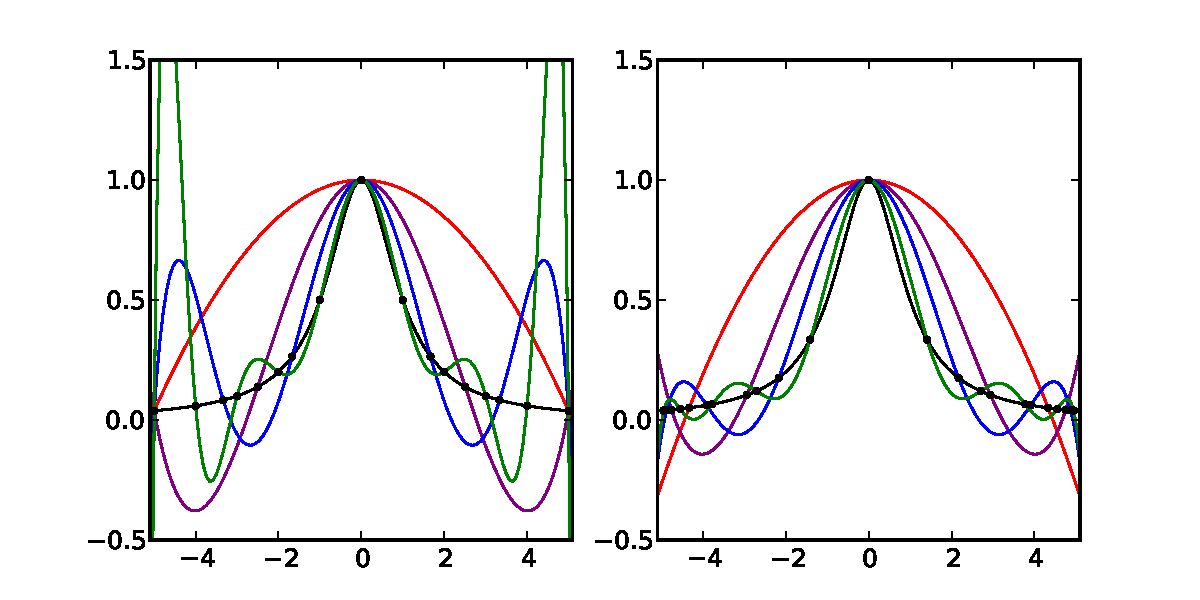
\includegraphics[width=\textwidth]{plots/runge_lagrange}
  \caption{Lagrange-Interpolation der Rungefunktion $1/(1+x^2)$
    (schwarze Linie). Im linken Graph sind die Stützstellen
    äquidistant gewählt (markierte Punkte), die farbigen Linien sind
    die interpolierenden Polynome durch 3 (rot), 5 (lila), 7 (blau)
    und 11 (grün) Stützstellen. Mit steigender Ordnung wird die
    Interpolation am Rand immer schlechter, das Polynom 10. Ordnung
    erreicht Werte bis nahe an zwei. Im rechten Graph sind
    für die gleichen Ordnungen Chebyshev-Stützstellen gewählt worden,
    die den Interpolationsfehler minimieren.}
  \label{fig:runge}
\end{figure}

Wie besprochen ist eine abgeschnittene Taylorreihe nur im
Entwicklungspunkt exakt (dann allerdings auch die Ableitungen),
innerhalb des Konvergenzradius nur eine Annäherung, und außerhalb des
Konvergenzradius sogar divergent.  Oft möchte man aber eher für einen
größeren Wertebereich eine gute (oder wenn möglich exakte) Darstellung
der Funktion haben.

Eine Möglichkeit dazu bietet die Polynom- oder
Lagrangeinterpolation. Dazu legt man eine Anzahl von Punkten im
gewünschten Wertebereich fest (die sogenannten \emph{Stützstellen}).
Wie sich zeigt, gibt es dann genau ein Polynom, dass die Funktion an
diesen Punkten exakt interpoliert. Genauer: seien Punkte $(x_i, y_i)$,
$i=0(1)n-1$ gegeben mit $x_i$ paarweise verschieden. Dann gibt es
genau ein Polynom $P(x)=\sum_{k=0}^{n-1} a_kx^{k}$ vom Grad $n-1$, so
dass $P(x_i) = y_i$, da die Gleichung
\begin{equation}
  \begin{split}
    y_1 &= P(x_0) = a_0 + a_1 x_0 + \cdots + a_{n-1}x_0^{n-1}\\
    \vdots\\
    y_n &= P(x_{n-1}) = a_0 + a_1 x_{n-1} + \cdots + a_{n-1}x_{n-1}^{n-1}
  \end{split}
  \label{eq:interpol}
\end{equation}
genau eine Lösung hat.

Leider ist aber nicht gewährleistet, dass mit steigender Anzahl von
Punkten die Funktion auch zwischen den Stützstellen immer besser
angenähert wird. Tatsächlich hat Runge ein einfaches Beispiel
angegeben, nämlich die Rungefunktion $1/(1+x^2)$, für die die Näherung
mit steigender Anzahl an äquidistanten Punkten immer schlechter wird,
siehe Abbildung~\ref{fig:runge}.

Bei der etwas allgemeineren Hermite-Interpolation können an den
Stützstellen neben den Funktionswerten auch Ableitungen vorgegeben
werden. Das eindeutige interpolierende Polynom hat dann einen Grad,
der der Gesamtanzahl an vorgegebenen Funktionswerten und Ableitungen
entspricht. Ist zum Beispiel nur eine Stützstelle $x_0$ gegeben und
neben dem Funktionswert $n$ Ableitungen, so entspricht das
Hermite-Polynom genau den ersten $n+1$ Termen der Taylorreihe.

Das interpolierende Polynom kann nicht nur zur Interpolation verwendet
werden, also der Bestimmung an Punkten zwischen den Stützstellen,
sondern --- mit Vorsicht --- auch zur Extrapolation, also um Werte
außerhalb des Bereichs zu bestimmen. Da bei der Hermite-Interpolation
auch die Ableitungen insbesondere am Rand kontrolliert werden können,
ist diese hier tendenziell vorteilhafter. Extrapolation spielt eine
wichtige Rolle, wenn eine direkte Auswertung der Zielfunktion
numerisch zu teuer oder unmöglich wird. Bei Computersimulationen tritt
dies insbesondere in der Nähe von kritischen Punkten auf.

In SciPy liefert die Funktion \scipy{scipy.interpolate.lagrange(x, y)}
das interpolierende Polynom durch die Stützstellen (\argd{x[i]},
\argd{y[i]}).

\subsection{\keyword{Lagrangepolynome}}

Die Koeffizienten $a_i$ können im Prinzip als Lösung von
Gleichung~\eqref{eq:interpol} mit geeigneten Lösern für lineare
Gleichungssysteme gefunden werden, was im allgemeinen allerdings recht
langsam ist. Daher benutzt man besser eine direkte Darstellung mit
Hilfe der \emph{Lagrangepolynome}, die wie folgt definiert sind:
\begin{equation}
  \label{eq:lagrange}
  L_i(x) = \prod_{k\neq i} \frac{x-x_k}{x_i-x_k}.
\end{equation}
Die Polynominterpolation wird daher auch Lagrange-Interpolation
genannt.  Wie man leicht sieht, gilt $L_i(x_k) = \delta_{ik}$, so dass
das Polynom\index{interpolierendes Polynom>Lagrangedarstellung}
\begin{equation}
  P(x) = \sum_{i=1}^n y_i\,L_i(x)
\end{equation}
das eindeutige interpolierende Polynom durch $(x_i, y_i)$
ist.

\index{interpolierendes Polynom>baryzentrische Darstellung}
Diese Darstellung ist allerdings für praktische Zwecke nur sinnvoll,
wenn sich die Stützstellen $x_i$ nicht ändern, da die Bestimmung der
Lagrangepolynome $L_i(x)$ zeitaufwändig ist. Geeigneter ist die
\emph{baryzentrische Darstellung}
\begin{equation}
P(x) = \sum_{i=0}^{n-1} y_i\, \mu_i \; \Big/ \; \sum_{i=0}^{n-1}
\mu_i\quad\text{mit}\quad
\mu_i := \frac{1}{x-x_i}\prod_{k\neq i}\frac{1}{x_i-x_k},
\end{equation}
bei der lediglich der Quotient zweier rationaler Funktionen gebildet
werden muss. 

\subsection{\keyword{Neville-Aitken-Schema}}

Das rekursive Neville-Schema ist eine effiziente Möglichkeit, das
interpolierende Polynom auszuwerten ohne es tatsächlich zu
berechnen. Das ist nützlich, wenn nur wenige Auswertungen nötig sind,
wie zum Beispiel beim Romberg-Integrationsverfahren, bei dem zur
Schrittweite 0 extrapoliert wird.

Wir definieren $P_{i,k}$ als das interpolierende Polynom der Ordnung
$k-1$ durch die Stützstellen $x_j, j=i(1)i+k-1$.  Gesucht ist der Wert
$P(x)=P_{0,n}(x)$ des interpolierenden Polynoms an der Stelle $x$.
Dann ist
\begin{align}
  P_{i,1}(x)&=y_i \quad\text{für}\, i=0(1)n-1
  \intertext{und}
  \label{eq:divdiff}
  P_{i,k}(x)&= \frac{P_{i,k-1}(x)(x_{i+k-1} - x) + P_{i+1,k-1}(x)(x -
    x_i)}{x_{i+k-1} - x_i} \quad\text{für}\, k=2(1)n, i=0(1)n-k,
\end{align}
da ja an den inneren Stützstellen $x_l$, $l=i+1(1)i+k-2$,
$P_{i,k-1}(x_l)=P_{i+1,k-1}(x_l) = y_l$ gilt, und per Konstruktion
$P_{i,k}(x_i)=y_i$ und $P_{i,k}(x_{i+k-1})=y_{i+k-1}$. Durch
sukzessives Berechnen zunächst der $P_{i,2}(x)$, dann der
$P_{i,3}(x)$, usw.\ lässt sich das interpolierende Polynom bequem an
einer fixen Stelle auswerten. Als (Neville-)Schema sieht das so aus:
\begin{center}
  \begin{tikzpicture}[on grid=true, node distance=1.5em and 10em]
    \node (u01) {$y_0$};
    \node[below=of u01] (u11) {$y_1$};
    \node[below=of u11] (u21) {$y_2$};
    \node[below=of u21] (u31) {$y_3$};
    \node[below=of u31] (u41) {$\vdots$};
  
    \node[right=of u11] (u02) {$P_{0,2}(x)$};
    \node[below=of u02] (u12) {$P_{1,2}(x)$};
    \node[below=of u12] (u22) {$P_{2,2}(x)$};
    \node[below=of u22] (u32) {$\vdots$};
  
    \node[right=of u12] (u03) {$P_{0,3}(x)$};
    \node[below=of u03] (u13) {$P_{1,3}(x)$};
    \node[below=of u13] (u23) {$\vdots$};

    \node[right=of u13] (u04) {$P_{0,3}(x)$};
    \node[below=of u04] (u14) {$\vdots$};

    \draw[->] (u01) -- (u02);
    \draw[->] (u11) -- (u02);
    \draw[->] (u11) -- (u12);
    \draw[->] (u21) -- (u12);
    \draw[->] (u21) -- (u22);
    \draw[->] (u31) -- (u22);

    \draw[->] (u02) -- (u03);
    \draw[->] (u12) -- (u03);
    \draw[->] (u12) -- (u13);
    \draw[->] (u22) -- (u13);

    \draw[->] (u03) -- (u04);
    \draw[->] (u13) -- (u04);
  \end{tikzpicture}
\end{center}
wobei die Pfeilpaare dividierte Differenzen gemäß \eqref{eq:divdiff} bedeuten.

\subsection{Newtonsche Darstellung}
\index{interpolierendes Polynom>Newtonsche Darstellung}

Wir betrachten nun die Polynome $P_{0,k}$ des Nevilleschemas. Es gilt
offenbar
\begin{equation}
  P_{0,k}(x) - P_{0,k-1}(x) = \gamma_k(x-x_0)\cdots(x-x_{k-2}),
\end{equation}
da die beiden Polynome in den Stützstellen $x_0,\ldots,x_{k-2}$
übereinstimmen und die Differenz ein Polynom vom Grad $k-1$ ist, also
höchstens $k-1$ Nullstellen hat. Weiter ist $\gamma_k$ der führende
Koeffizient des Polynoms $P_{0,k}(t)$, da $P_{0,k-1}(t)$ ja einen
niedrigeren Grad hat. Daraus ergibt sich die folgende \emph{Newtonsche
  Darstellung} des interpolierenden Polynoms:
\begin{equation}
  \begin{split}
    P_{0,n}(x) &= y_0 + \sum_{k=2}^{n} P_{0,k}(x) - P_{0,k-1}(x)\\
    &= y_0 + \gamma_2(x-x_0) + \gamma_3(x-x_0)(x-x_1) + \cdots
    + \gamma_n(x-x_0)\cdots(x-x_{n-2})\\
    &= y_0 + (x-x_0)\biggl(\gamma_2 + (x-x_1)\Bigl(\gamma_3 + \cdots
    \bigl(\gamma_{n-1} + (x-x_{n-2})\gamma_n\bigr)\cdots\Bigr)\biggr).
  \end{split}
\end{equation}
Die letztere Umformung zeigt, dass sich die Newtonsche Darstellung
effizient mit einem leicht abgewandelten Hornerschema auswerten lässt:
\begin{lstlisting}
def horner(x0, x, gamma):
    r = 0
    for k in range(len(x)-1, -1, -1):
        r = r*(x0-x[k]) + gamma[k];
    return r
\end{lstlisting}

Die Koeffizienten $\gamma_i$, $i=2(1)n$ lassen sich dabei bequem mit
dem Nevilleschema bestimmen. $\gamma_k$ ist ja der höchste Koeffizient
von $P_{0,k}$ ist, der sich leicht aus \eqref{eq:divdiff} berechnen
lässt. Wenn $\gamma_{i,k}$ den führenden Koeffizienten des Polynoms
$P_{i,k}$ bezeichnet, so erhalten wir das Nevilleschema
\begin{align}
  \gamma_{i,1} &= y_i \quad\text{für}\, i=0(1)n-1\quad\text{und}\\
  \gamma_{i,k}&= \frac{\gamma_{i+1,k-1} - \gamma_{i,k-1}}{x_{i+k-1} -
    x_i}
  \quad\text{für}\, k=2(1)n, i=0(1)n-k.
\end{align}
Da letztlich nur die $\gamma_{0,k}$ interessant sind, also die obere
Diagonale des Nevilleschemas, benötigt man für die Berechnung nur
einen Vektor
\begin{equation}
  \gamma' = \left(\gamma_{0,1},\gamma_{0,2},\ldots,\gamma_{0,k-1},
    \gamma_{0,k},\gamma_{1,k},\ldots,\gamma_{n-k,k}\right),
\end{equation}
der wie folgt berechnet wird:
\begin{lstlisting}
def neville(x, y):
    n = len(x)
    gamma = y.copy()
    for k in range(1, n):
        for i in range(n-k-1, -1, -1):
            gamma[i+k] = (gamma[i+k] - gamma[i+k-1])/(x[i+k] - x[i])
    return gamma
\end{lstlisting}
Man beachte, dass die Schleife über $i$ herunterläuft, um benötigte
Werte nicht zu überschreiben.

\subsection{\keyword{Chebyshev-Stützstellen}}

Bis jetzt haben wir wenig zur Wahl der Stützstellen gesagt. Oft liegt
es auch nahe, äquidistante Stützstellen zu verwenden wie im
Fadenpendel-Beispiel. Man kann allerdings zeigen, dass die
Chebyshev-Stützstellen den Fehler der Polynominterpolation minimieren.
Diese sind definiert als die Nullstellen der Polynome (!)
\begin{equation}
  \label{eq:chebyshev}
  T_n(\cos\phi) = \cos(n\phi),
\end{equation}
die offensichtlich zwischen -1 und 1 liegen und daher geeignet
skaliert werden müssen für die Interpolation in einem allgemeinen
Intervall. Die Chebyshev-Polynome $T_n$, $n\ge 0$, bilden eine
orthogonale Basis der Funktionen über $[-1,1]$ bezüglich des mit
$1/\sqrt{1-x^2}$ gewichteten Skalarprodukts. Daher kann jede genügend
glatte Funktion auf $[-1:1]$ als eine Reihe
\begin{equation}
  f(x) = \sum_{n=0}^\infty a_n T_n(x)
\end{equation}
dargestellt werden, die sogenannte Chebyshev-Reihe (siehe auch z.B.
\textcite{abramowitz70a}).

 Explizit sind diese Nullstellen gegeben durch
\begin{equation}
  x_{k,n} = \cos\left(\frac{2k+1}{2n}\pi\right),\quad k=0(1)n-1.
\end{equation}
Wird die Rungefunktion mit Chebyshevstützstellen interpoliert, so
konvergiert das interpolierende Polynom, im Gegensatz zu äquidistanten
Stützstellen.

\section{Splines}
\index{Spline}
\index{Interpolation>Spline-}

Wie wir gesehen haben, kann unter ungünstigen Umständen die Güte der
Polynominterpolation mit steigender Anzahl an Stützstellen sinken, vor
allem, wenn diese äquidistant verteilt sind. Oft ist das aber nicht zu
vermeiden, zum Beispiel, wenn die Daten in einem Experiment regelmäßig
gemessen werden. Das Problem ist, das die Koeffizienten des Polynoms
global gelten, sich glatte Funktionen aber nur lokal wie ein Polynom
verhalten (Taylorentwicklung!). Daher ist es günstiger, statt der
gesamten Funktion nur kleine Abschnitte durch Polynome zu nähern.

Der einfachste Fall einer solchen Näherung ist die \emph{lineare
  Interpolation}\index{Interpolation>lineare}, bei der die
Stützstellen durch Geraden, also Polynome vom Grad 1, verbunden
werden. Sind die Stützstellen $(x_i, y_i)$, $i=1(1)n$ gegeben, so ist
der lineare interpolierende Spline
\begin{equation}
  P_1(x) = \frac{(x_{i+1} - x)y_i + (x - x_i)y_{i+1}}
  {x_{i+1}-x_i}
  \quad\text{für}\, x_i \le x < x_{i+1}.
\end{equation}

\begin{figure}
  \centering
  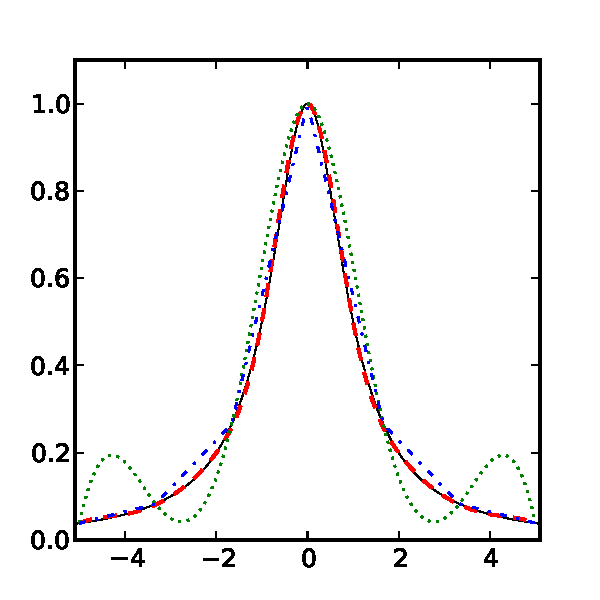
\includegraphics[width=0.5\textwidth]{plots/splines}
  \caption{Spline-Interpolation der Rungefunktion (durchgezogene
    schwarze Linie). Die gestrichelte blaue Linie ist die lineare
    Spline-Interpolierende mit 7 Stützstellen, die anderen Kurven sind
    kubische Splines mit 7 (grün gepunktet) und 11 Stützstellen (rot
    gestrichelt). Mit 11 Stützstellen ist der Spline von der
    Rungefunktion praktisch nicht mehr zu unterscheiden.}
  \label{fig:spline}
\end{figure}

Diese Funktionen sind aber an den Stützstellen im allgemeinen nicht
differenzierbar. Soll die Interpolierende differenzierbar sein, müssen
Polynome höherer Ordnung genutzt werden. Solche stückweise definierten
Polynome heißen \emph{Splines} --- das englische Wort Splines
bezeichnete dünne Latten, die vor dem Computerzeitalter benutzt
wurden, um glatte, gebogene Oberflächen vor allem für Schiffsrümpfe zu
entwickeln. Der wichtigste Spline ist der \emph{kubische} oder
\emph{natürliche}
Spline\index{Spline>kubisch}\index{Spline>natürlich}, der aus
Polynomen dritten Grades zusammengesetzt und zweifach stetig
differenzierbar ist. Seine allgemeine Form ist
\begin{equation}
  P_3(x) = y_i + m_i(x-x_i) + \frac{1}{2}M_i(x-x_i)^2 + \frac{1}{6}\alpha_i(x-x_i)^3
  \quad\text{für}\, x_i \le x < x_{i+1}.
\end{equation}
Da die zwei rechten und linken zweiten Ableitungen an den Stützstellen
übereinstimmen müssen, gilt
\begin{equation}
  \alpha_i = \frac{M_{i+1} - M_i}{x_{i+1} - x_i}.
\end{equation}
Aus der Gleichheit der Funktionswerte an den Stützstellen ergibt sich
\begin{equation}
  m_i = \frac{y_{i+1} - y_i}{x_{i+1}-x_i} -
  \frac{1}{6}(x_{i+1}-x_i)(2M_i + M_{i+1}).
\end{equation}
Aus der Gleichheit der ersten Ableitungen ergibt sich schließlich ein
Gleichungssystem für die $M_i$. Hier kommen in den Gleichungen
gleichzeitig $M_{i-1}$, $M_i$ und $M_{i+1}$ vor, daher müssen für die
Randwerte weitere Vorgaben gemacht werden. Sollen die Splines am Rand
festgelegte 2. Ableitungen $M_0$ und $M_n$ haben, so hat das
Gleichungssystem die Form
\begin{equation}
  \label{eq:spline1}
  \begin{pmatrix}
    2      & \lambda_1 &           &           &           &         0 \\
    \mu_2  & 2         & \lambda_2 \\
           &           & \ddots    & \ddots    & \ddots \\
           &           &           & \mu_{n-2}  & 2         & \lambda_{n-2} \\
    0      &           &           &           & \mu_{n-1}  & 2         \\
  \end{pmatrix}
  \begin{pmatrix}
    M_1\\
    M_2\\
    \vdots\\
    M_{n-2}\\
    M_{n-1}
  \end{pmatrix} \,=\,
  \begin{pmatrix}
    6S_1 - \mu_1 M_0\\
    6S_2\\
    \vdots\\
    6S_{n-2} \\
    6S_{n-1} -  \lambda_{n-1} M_n
  \end{pmatrix},
\end{equation}
mit
\begin{equation}
  \lambda_i = \frac{x_i - x_{i-1}}{x_{i+1} - x_{i-1}},\quad
  \mu_i = \frac{x_{i+1}-x_i}{x_{i+1} + x_{i-1}}\quad\text{und}\quad
  S_i = \frac{\frac{y_{i+1}-y_i}{x_{i+1} -
      x_i} - \frac{y_i-y_{i-1}}{x_i - x_{i-1}}}{x_{i+1}-x_{i-1}}.
\end{equation}
Auch periodische Funktionen können kubisch interpoliert werden, wobei
dann die zusätzliche Bedingungen durch die Kontinuität über die periodische
Grenze hinweg gegeben sind. Die Gleichungen für $\alpha_i$ und $m_i$
sind dabei unverändert, nur das Gleichungssystem wird
\begin{equation}
  \label{eq:spline2}
  \begin{pmatrix}
    2      & \lambda_1 &           &           &           &      \mu_1 \\
    \mu_2  & 2         & \lambda_2 &           & 0\\
           &           & \ddots    & \ddots    & \ddots \\
           & 0          &           & \mu_{n-2}  & 2         & \lambda_{n-2} \\
    \lambda_{n-1} &           &           &           & \mu_{n-1}  & 2         \\
  \end{pmatrix}
  \begin{pmatrix}
    M_1\\
    M_2\\
    \vdots\\
    M_{n-2}\\
    M_{n-1}
  \end{pmatrix} \,=\,
  \begin{pmatrix}
    6S_1\\
    6S_2\\
    \vdots\\
    6S_{n-2} \\
    6S_{n-1}
  \end{pmatrix},
\end{equation}
wobei die Funktion als $x_n-x_1$-periodisch mit $y_1=y_n$
vorausgesetzt wird. Abbildung~\ref{fig:spline} zeigt die
Spline-Interpolation der Rungefunktion, die für diesen
Interpolationstyp keine Probleme zeigt.

Die Gleichungssysteme \eqref{eq:spline1} und \eqref{eq:spline2} sind
sehr gut konditioniert und mit einem einfachen Gleichungslöser zu
behandeln.  Zum Beispiel ist die Gauß-Elimination ist für die hier
auftretenden einfachen Bandstrukturen sehr effizient. In SciPy gibt es
selbstverständlich bereits eine fertige Routine für die
Spline-Interpolation, nämlich \scipy{scipy.interpolate.interp1d(x, y,
  kind)}. (\argd{x},\argd{y}) sind dabei die Stützstellen, und
\argd{kind} eine Zeichenkette, die den Typ des Splines
bestimmt. Mögliche Werte sind zum Beispiel "`linear"' und "`cubic"'
für lineare bzw..\ kubische interpolierende Splines.

\section{Ausgleichsrechnung, Methode der kleinsten Quadrate}
\index{Ausgleichsrechnung}
\index{Fitting}
\index{Methode der kleinsten Quadrate}

\begin{figure}
  \centering
  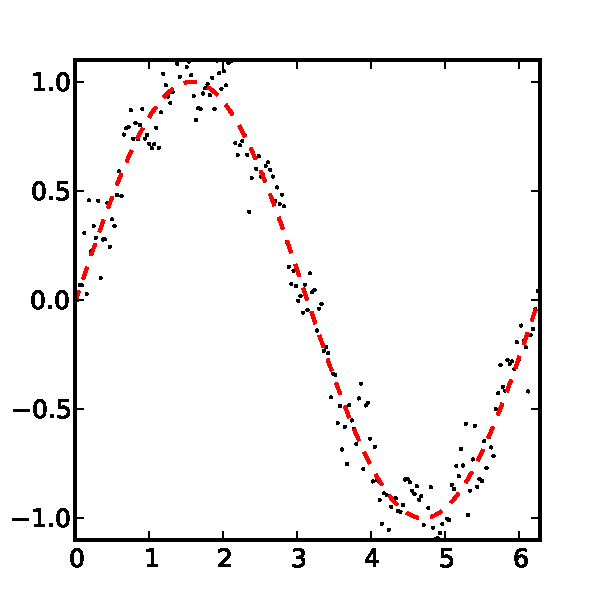
\includegraphics[width=0.5\textwidth]{plots/leastsq}
  \caption{Methode der kleinsten Quadrate zum Fitten der Sinusfunktion
    $y=\sin(x)$. 200 Datenpunkte zwischen 0 und $2\pi$ wurden als
    $\sin(x) + 0,1\,\sin(10 x) + \xi$ erzeugt, wobei $\xi$ eine
    Gauß-verteilte Pseudozufallsvariable mit Varianz $0,01$ war. Die
    resultierende Sinusfunktion (rot gestrichelt) hat die Form $a
    \sin(bx+c)$, wobei die Koeffizienten auf gut 2\% Genauigkeit
    $a=b=1$ und $c=0$ entsprechen. Die kleine höherfrequente
    Schwingung kann durch einen Fit allerdings nicht zuverlässig
    erkannt werden.}
  \label{fig:leastsq}
\end{figure}

Interpolierende Polynome, Taylorreihen und Splines haben gemeinsam,
das diese exakt durch die gegebenen Stützstellen verlaufen. Oftmals
ist das aber gar nicht gewünscht, da die Daten selbst nicht exakt
sind, zum Beispiel wenn diese aus einem Experiment oder einer
Simulation stammen. In diesem Fall hat man üblicherweise eine
Vorstellung, welche funktionelle Form die Daten annehmen, und möchte
nun wissen, mit welchen Parametern diese Funktion am besten mit den
Daten verträglich ist. Dazu muss man den Parametersatz bestimmen, so
dass der Abstand der Daten von der Funktion minimiert wird.

Seien also wieder Daten $(x_i, y_i)$, $i=1(1)n$ und eine Funktion
$f_v(x)$ gegeben. Gesucht ist dann derjenige Parametervektor $v$, der
die Abweichung
\begin{equation}
  \label{eq:leastsq}
  \Delta(v) = \sum_i (f_v(x_i) - y_i)^2
\end{equation}
minimiert. Dieses Verfahren wird auch Methode der kleinste Quadrate
genannt, da ja die quadrierten Abweichungen minimiert werden
sollen. Ist $f_{a,b}(x) = ax + b$ eine Gerade, spricht man auch von
\emph{linearer Regression}\index{lineare Regression}. In diesem Fall lässt
sich das Optimum einfach bestimmen, da
\begin{equation}
  0 = \frac{d}{da} \Delta(a,b) = \sum_i 2 (a x_i + b - y_i)x_i
  = 2N \left(a  \left<x_i^2\right> + b \left<x_i\right> -
    \left<y_ix_i\right> \right)
\end{equation}
und
\begin{equation}
  0 = \frac{d}{db} \Delta(a,b) = \sum_i 2 (a x_i + b - y_i)
  = 2N \left(a  \left<x_i\right> + b - \left<y_i\right> \right),
\end{equation}
wobei $\left<\cdot\right>$ den Mittelwert über alle Datenpunkte
bedeutet. Daraus ergibt sich
\begin{equation}
  a = \frac{\left<y_ix_i\right> -
    \left<y_i\right>\left<x_i\right>}{\left<x_i^2\right>-\left<x_i\right>^2}
  \quad\text{und}\;
  b = \left<y_i\right> - a \left<x_i\right>,
\end{equation}
was sich einfach auf dem Computer berechnen lässt.

Auch für quadratische und andere einfache Funktionen lassen sich die
Koeffizienten geschlossen darstellen, aber bei allgemeinen Funktionen
ist dies nicht immer der Fall. Dann muss die nichtlineare
Optimierungsaufgabe \eqref{eq:leastsq} numerisch gelöst werden, was
wir später behandeln werden. Für den Moment genügt uns, dass SciPy die
Funktion \scipy{scipy.optimize.leastsq(delta, v0, (x, y))} dafür
bereitstellt. \argd{(x, y)} sind dabei die Ausgangsdaten, die hier zu
einem Tupel zusammengefasst sind. \argd{v0} ist der Startwert für die
Berechnung, der nicht zu weit vom (unbekannten) Optimum entfernt
liegen darf. \argd{delta} ist eine Python-Funktion, die als Argumente
$v$, $x_i$ und $y_i$ nimmt und $f_v(x_i) - y_i$ zurückliefert.  Da
$f_v(x)$ eine beliebig komplizierte Form annehmen kann, ist diese
Aufgaben im allgemeinen nicht lösbar, allerdings funktioniert ein
solcher \emph{Fit} für einfache Funktionen meistens recht
gut. Abbildung~\ref{fig:leastsq} zeigt einen solchen Funktionsfit an
eine verrauschte Sinusfunktion, die mit 200 Datenpunkten auf etwa 2\%
genau gefittet werden kann. Man beachte, das der Ausgangswert für den
Fit mit Hilfe der SciPy-Funktion \lstinline!leastsq! $a=0$, $b=1$,
$c=0$ war; beim Startwert $a=0$, $b=0$, $c=0$ bricht das Verfahren
ab. Das zeigt, dass man tatsächlich nicht zu weit vom Optimum starten
kann, was ein gewisses Verständnis der Zielfunktion voraussetzt.

Ist die Funktionsform, die den Daten zugrundeliegt, unbekannt, ist es
normalerweise keine gute Idee, die Form zu raten. Generell sollte auch
die Anzahl der Parameter sehr klein sein, da sich sonst fast alles
"`gut"' fitten lässt ("`With four parameters I can fit an elephant and
with five I can make him wiggle his trunk."' --- J. von Neumann).

Soll aber zum Beispiel für Visualisierungszwecke eine ansprechende
Kurve entlang der Daten gelegt werden, deren tatsächliche Abhängigkeit
unbekannt ist, dann sind \emph{Pad\'e-Funktionen} oft eine gute
Wahl. Diese haben die Gestalt $P(x)/Q(x)$, wobei $P$ und $Q$ zwei
Polynome mit paarweise verschiedenen Nullstellen sind. Üblicherweise
lassen sich schon niedrigen Polynomgraden ansprechende Fits finden,
sofern die Grade der beiden Polynome in etwa gleich gewählt werden.

\section{Fourierreihen}

Bis jetzt waren unsere Näherungsfunktionen auf Polynomen basierend, da
diese einerseits vom Computer verarbeitet werden können und
andererseits aufgrund der Taylorentwicklung glatte Funktionen meist
gut approximieren. Für periodische Funktionen sind Polynome aber an
sich erst einmal wenig geeignet, da sie selbst nicht periodisch
sind. Splines können zwar auch periodisch gemacht werden, aber
trotzdem sind trigonometrische Funktionen besser geeignet, um
periodische Funktionen darzustellen. Fourierreihen und
-transformationen stellen Funktionen als trigonometrische Reihen dar,
die meist gut konvergieren und darüber hinaus einige nützliche
Eigenschaften haben.

Es gibt zwei Hauptanwendungen der Fourierdarstellung: die Analyse und
Aufbereitung periodischer Signale und die Lösung von
Differentialgleichungen.  Bei periodischen Signalen dient die
Fourierdarstellung zur Analyse des \emph{Spektrums} des Signals.
Diese gibt nützliche Informationen über die charakteristischen
Zeitskalen von Strukturen im Signal, zum Beispiel die Tonhöhe und die
Obertonreihe eines Instruments. In dieser Frequenzdarstellung lassen
sich auch gezielt einzelne Frequenzen dämpfen, was Rauschen
unterdrücken kann und im ursprünglichen Funktionsraum teure Faltungen
erfordert.  Bei Differentialgleichungen nutzt man aus, dass die
Ableitung im Frequenzraum eine algebraische Operation ist, und die
Differentialgleichung somit in eine gewöhnliche algebraische (und oft
sogar lineare) übergeht.

\subsection{Komplexe Fourierreihen}
\index{Fourierreihen>komplexe}
\index{Fouriertransformation>komplexe}
Wir betrachten eine periodische Funktion $f(t)$ mit $f(t+T) = f(t)$
für alle $t\in\RR$, d.h. $f$ hat Periode $T$. Dann ist die
Fourierdarstellung von $f$ gegeben durch
\begin{equation}
  \label{eq:fourier}
  f(t) = \sum_{n\in\ZZ} \hat{f}_n e^{i n\omega t}
\end{equation}
mit $\omega=2\pi/T$. Die Koeffizienten $\hat{f}_n$ lassen sich
berechnen als
\begin{equation*}
  \label{eq:fouriercoeff}
  \hat{f}_n = \frac{1}{T}\int_0^T f(t)e^{-i n\omega t}\, dt
\end{equation*}
und sind im allgemeinen komplex, auch wenn $f$ reellwertig ist. Die
Beiträge $\hat{f}_{\pm n}$ haben dieselbe Frequenz $\pm n/T$,
unterscheiden sich aber in ihrer Phase. Die \emph{Leistung} zu dieser
Frequenz ist $\hat{f}_{n}\hat{f}_{-n}$.

\eqref{eq:fourier} lässt sich auch so lesen, dass
\begin{equation}
  e^{-i n\omega t} = \cos(n \omega t) + i \sin(n \omega t)
\end{equation}
eine orthonormale Basis bezüglich des Skalarprodukts
\begin{equation}
  \label{eq:l2scalar}
  (f, g) = \frac{1}{T}\int_0^T f(t)\overline{g(t)}\,dt
\end{equation}
bilden. Ähnlich wie ein Vektor im $\RR^n$ wird die Funktion $f$ also
durch die Fouriertransformation in ihre Schwingungskomponenten
zerlegt.  Insbesondere sind die Fourierkoeffizienten linear in der
Funktion, d.h.
\begin{equation}
  \widehat{f+\lambda g}_n = \hat{f}_n +\lambda \hat{g}_n.
\end{equation}

Die Voraussetzungen für die Konvergenz der Fourierreihe sind sehr
schwach - solange die Funktion wenigstens quadratintegrabel ist,
konvergiert die Fourierreihe fast überall, d.h.
\begin{equation}
  \left\lVert f(t) - \sum_{n=-N}^N \hat{f}_n e^{i n\omega t} \right\rVert \xrightarrow{N\to\infty} 0.
\end{equation}
Daneben ist die Transformation $f\to\hat{f}$ eine \emph{Isometrie},
genauer gilt das \emph{\keyword{Parsevaltheorem}}
\begin{equation}
  \sum_{n\in\ZZ} \lvert\hat{f}_n\rvert^2 =
  \frac{1}{\omega}\int_0^t \lvert f(t)\rvert^2\,dt.
\end{equation}
Das Parsevaltheorem besagt auch, dass die Restbeiträge von großen $n$
immer kleiner werden, so dass also eine abgeschnittene Fourierreihe
eine Approximation an die gesuchte Funktion darstellt. Anders als
abgeschnittene Taylorreihen, die nur in einer schmalen Umgebung um den
Aufpunkt exakt sind, konvergiert die Fourierreihe
gleichmäßig. Allerdings muss die abgeschnittene Fourierreihe im
allgemeinen keinen einzigen Punkt mit der Zielfunktion gemeinsam
haben, anders als Taylorreihen oder Splines.

Weiter gilt:
\begin{itemize}
\item Die Fourierreihe über einem Intervall $[0,T)$ kann aus der
  Fourierreihe für das Intervall $[0,2\pi)$ durch Streckung mit
  $\omega$ berechnet werden:
  \begin{equation}
    \widehat{f(t)}_n = \frac{1}{T}\int_0^T f(t)e^{-i n\omega t}\, dt
    = \frac{1}{2\pi}\int_0^{2\pi} f(t'/\omega)e^{-i n t'}\, dt',
  \end{equation}
\item Es gilt
  \begin{equation}
    \widehat{f(t + t_0)}_{n} = e^{i n \omega t_0} \widehat{f(t)}_{n}
  \end{equation}
  die Phase kann also nach Belieben verschoben werden. Die Leistung
  $\hat{f}_{n}\hat{f}_{-n}$ bleibt dabei natürlich erhalten.
\item Für die komplexe Konjugation gilt stets
  $\widehat{\overline{f}}_n = \overline{\hat{f}_n}$, da die
  Fouriertransformation ja linear ist.
\item Ist Funktion $f$ symmetrisch, also $f(t) = f(-t) = f(T-t)$, so ist
  $\hat{f}_{-n} = \hat{f}_n$, also $\hat{f}$ symmetrisch.
\item Ist Funktion $f$ ungerade, also $f(t) = -f(-t) = -f(T-t)$, so ist
  $\hat{f}_{-n} = -\hat{f}_n$, also $\hat{f}$ ungerade.
\item Ist Funktion $f$ reellwertig, also $f(t) = \overline{f(t)}$, so
  ist $\hat{f}_{-n} = \overline{\hat{f}_n}$. Allerdings sind die
  Fourierkoeffizienten im allgemeinen komplex!
\item 
  Ist die komplexwertige Funktion $f(t)=g(t) + ih(t)$ mit $g$, $h$
  reellwertig, gilt also
  \begin{equation}
    \hat{f}_{n}  + \hat{\overline{f}}_{n} = \widehat{2g}_{n}
    \quad\text{und}\;
    \hat{f}_{n}  - \hat{\overline{f}}_{n} = \widehat{2ih}_{n}.
  \end{equation}
  Dies bedeutet, dass sich die Fourierreihen zweier reellwertiger
  Funktionen zusammen berechnen und anschließend wieder trennen
  lassen. Da die Berechnung der Fourierkoeffizienten sowieso komplex
  erfolgen muss, erspart dies bei numerischer Auswertung eine
  Transformation.
\item Die Ableitung der Fourierreihe ist sehr einfach:
  \begin{equation}
    \frac{d}{dt}  f(t) = \sum_{n\in\ZZ} \hat{f}_n i n\omega e^{i n\omega
      t} = \sum_{n\in\ZZ} \widehat{\left(\frac{df}{dt}\right)}_n e^{i n\omega
      t}\quad\implies\quad \widehat{\left(\frac{df}{dt}\right)}_n= i n\omega\hat{f}_n.
  \end{equation}
\end{itemize}

\subsection{Reelle Fourierreihen}
\index{Fourierreihen>reelle}
\index{Fouriertransformation>reelle}

Da die Fourieranalyse besonders zur Analyse und Bearbeitung von
Messdaten genutzt wird, sind die Fourierreihen reellwertiger
Funktionen besonders wichtig. Ist die Funktion $f$ rellwertig, so ist
\begin{multline}
  \hat{f}_{n}e^{in \omega t} + \hat{f}_{-n}e^{-in \omega t} =
  \hat{f}_{n}e^{in \omega t} + \overline{\hat{f}_{-n}e^{in \omega t}}
  = 2\Re(\hat{f}_{n}e^{in \omega t})\\
  = 2\Re(\hat{f}_{n})\cos(n \omega t) - 2\Im(\hat{f}_{n})\sin(n \omega t).
\end{multline}
Daraus folgt, dass sich die Fourierreihe auch komplett reellwertig
schreiben lässt:
\begin{equation}
  f(t) = \frac{a_0}{2} + \sum_{n=1}^\infty a_n \cos(n\omega t) + b_n
  \sin(n\omega t)
\end{equation}
mit
\begin{align}
  a_n &= 2\Re(\hat{f}_{n}) = \frac{2}{T}\int_0^T f(t)\cos(n\omega t)\,
  dt
  \intertext{und}
  b_n &= -2\Im(\hat{f}_n) = \frac{2}{T}\int_0^T f(t)\sin(n\omega t)\,
  dt.
\end{align}
Für symmetrische Funktionen ist offenbar $b_n=0$, für ungerade
Funktionen $a_n=0$.

\begin{figure}
  \centering
  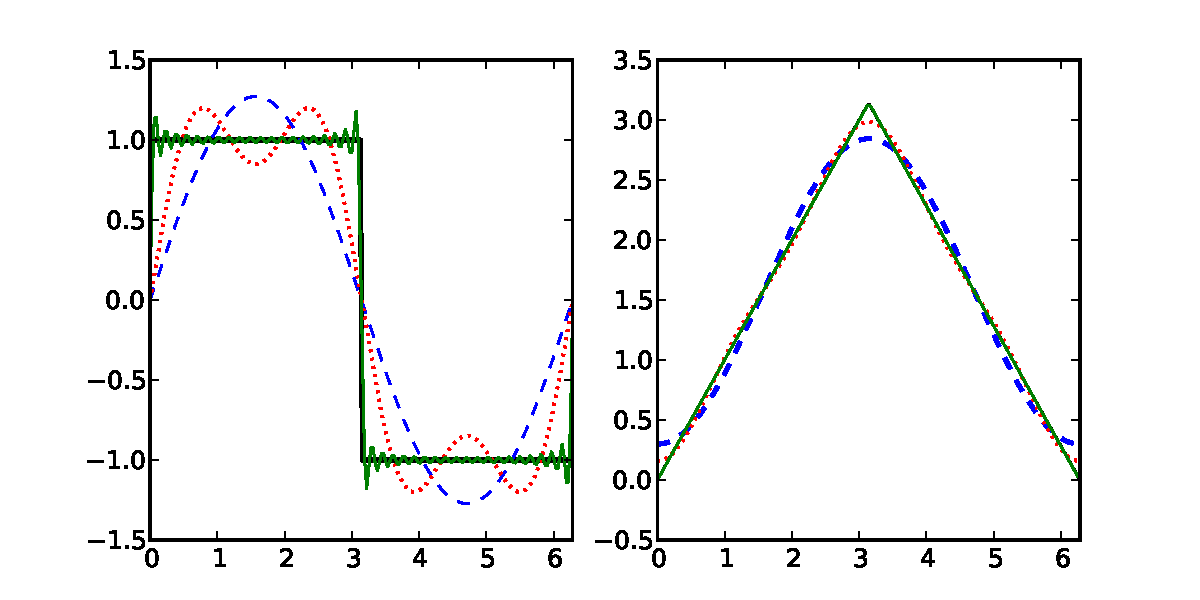
\includegraphics[width=\textwidth]{plots/fourier}
  \caption{Abgeschnittene Fourierreihen der Rechteckfunktion (links)
    und eines Dreieckpulses (rechts). Die Funktionen sind jeweils als
    schwarze durchgezogene Linien eingezeichnet, die Näherungen mit
    einem Term blau gestrichelt, mit zwei Termen rot gepunktet, und
    mit 20 Termen grün durchgezogen. Für den Dreieckpuls ist letztere
    Näherung nicht mehr von der Funktion zu unterscheiden, während der
    Rechteckpuls noch deutliche Artefakte an den Unstetigkeiten zeigt.}
  \label{fig:fourier}
\end{figure}
Einige reelle Fourierreihen sind zum Beispiel:
\begin{itemize}
\item Konstante $f(t) = f_0$:
  \begin{equation}
    a_0 = 2 f_0,\quad a_n,\,b_n= 0\quad\text{sonst}
  \end{equation}
\item Rechteckfunktion
  \begin{equation}
    f(t) = \begin{cases}
      1 &\text{für}\; 0 \le t < \frac{T}{2} \\
      -1  &\text{für}\; \frac{T}{2} \le t < T
    \end{cases}\\
    = \quad\frac{4}{\pi}\sum_{n=1}^\infty
    \frac{1}{2n-1}\sin\left((2n-1)\omega t\right)
  \end{equation}
\item kurzer Rechteckpuls. Wir betrachten nun die auf konstanten
  Flächeninhalt normierte Funktion
  \begin{equation}
    f_S(t) = \begin{cases}
      1/S &\text{für}\; 0 \le t < S \\
      0  &\text{für}\; S \le t < T
    \end{cases},
  \end{equation}
  deren Fourierreihe
  \begin{equation}
    f_s(t) =
    \quad \frac{1}{T} +
    \quad\frac{2}{T}\sum_{n=1}^\infty
    \frac{\sin(n\omega S)}{n\omega S}\cos(n\omega t) +
    \frac{1-\cos(n\omega S)}{n\omega S}\sin(n\omega t)
  \end{equation}
  ist. Je kleiner $S$ wird und damit der Träger von $f_S$, desto
  langsamer konvergiert ihre Fourierreihe, da die Funktion $\sin(x)/x$
  immer dichter an der Null ausgewertet wird. Für jede feste Frequenz
  $n$ gilt schließlich
  \begin{equation}
    \widehat{\left(f_S\right)}_n \xrightarrow{S\to 0} \frac{1}{T} = \hat\delta_n
    \quad\text{für alle}\;n\in\ZZ
  \end{equation}
  bzw.. $a_n\to 2/T$ und $b_n\to 0$. Die $\delta$-Funktion, die ja der
  formale Grenzwert der $f_S$ ist, und den kleinstmöglichen
  Träger hat, hat also in gewisser Weise die am schlechtesten
  (tatsächlich gar nicht!) konvergierende Fourierreihe.
\item Dreiecksfunktion
  \begin{equation}
    f(t) = \begin{cases}
      t      &\text{für}\; 0 \le t < \frac{T}{2} \\
      T - t  &\text{für}\; \frac{T}{2} \le t < T
    \end{cases}\quad=\quad\frac{\pi}{2} -
    \frac{4}{\pi}\sum_{n=1}^\infty
    \frac{1}{(2n-1)^2}\cos\left((2n-1)\omega t\right)
  \end{equation}
\end{itemize}
Genau wie die komplexe Fourierreihe lässt sich natürlich auch die
reelle Fourierreihe abschneiden, um Näherungen für Funktionen zu
bekommen, vergleiche Abbildung~\ref{fig:fourier}. Es fällt auf, das
die Fourierreihe besonders schlecht dort konvergieren, wo die Funktion
nicht differenzierbar ist bzw..\ einen Sprung aufweist.

\subsection{Diskrete Fouriertransformation}
\index{Fouriertransformation>diskrete}
\index{DFT}

\begin{figure}
  \centering
  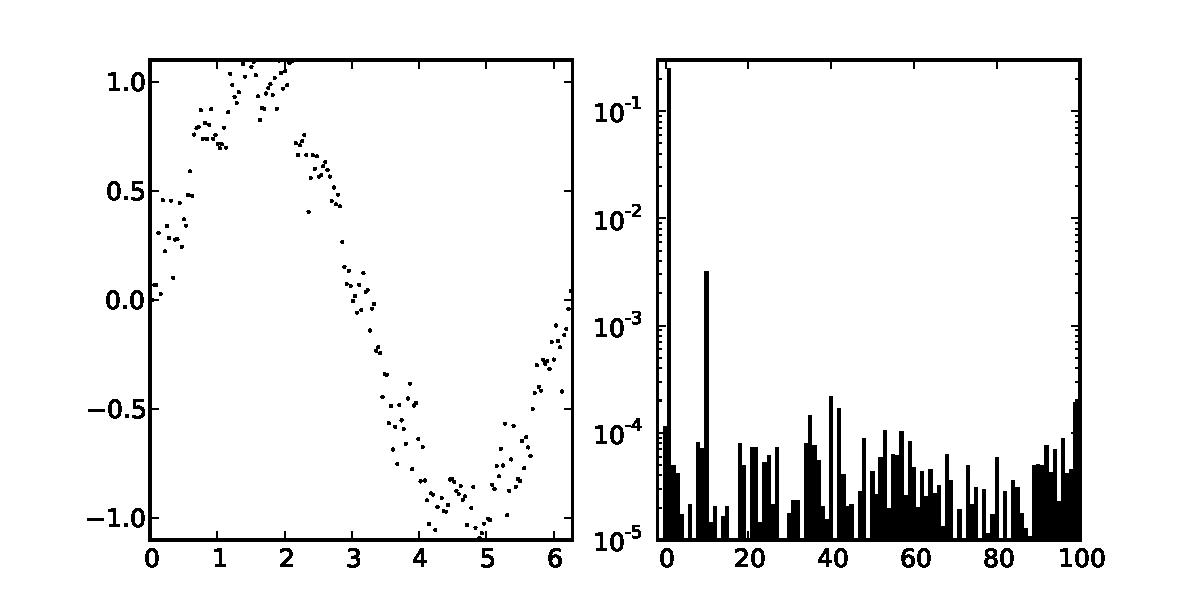
\includegraphics[width=\textwidth]{plots/fftsin}
  \caption{Diskrete Fouriertransformation von 200 diskreten
    Datenpunkten, die analog zu Abbildung~\ref{fig:leastsq} zwischen 0
    und $2\pi$ als $\sin(x) + 0,1\,sin(10 x) + \xi$ erzeugt wurden.
    Anders als der Funktionsfit erlaubt die DFT, auch die kleine
    zusätzliche Schwingung gut vom Rauschen zu unterscheiden. Im
    Graphen ist das Leistungsspektrum $\lvert DFT(k)\rvert^2$ gezeigt.
    Man erkennt die Amplitudenquadrate $0,25$ bei 1 und $0,01$ bei 10,
    auch wenn letztere Frequenz durch das Rauschen etwas an Intensität
    verloren hat.
  }
  \label{fig:fouriersin}
\end{figure}

\begin{figure}
  \centering
  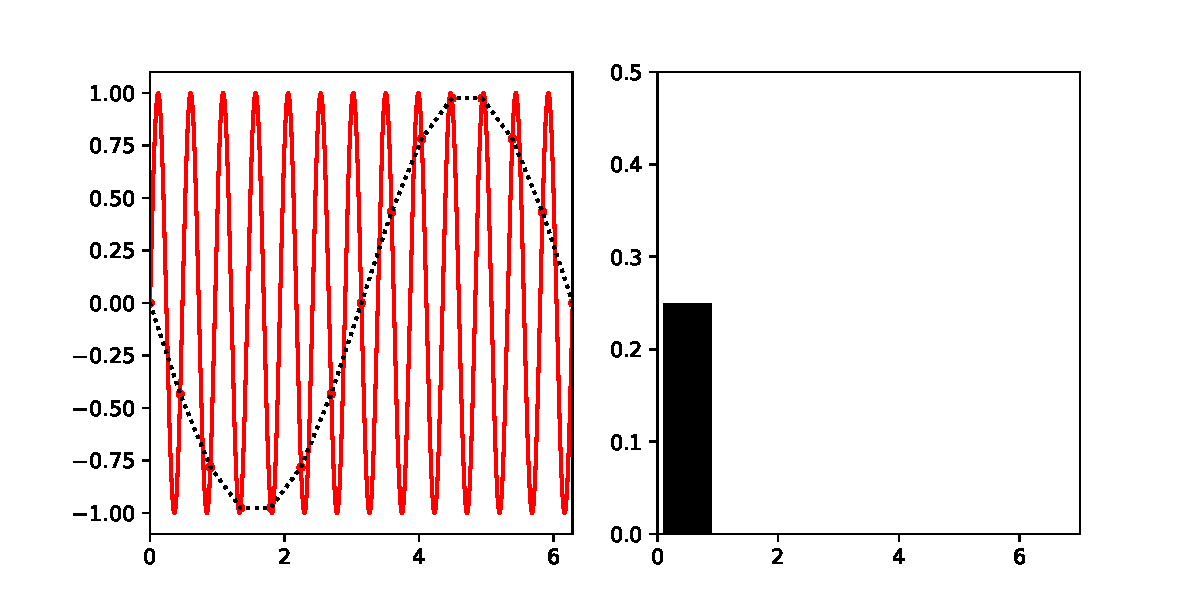
\includegraphics[width=\textwidth]{plots/fftalias}
  \caption{Diskrete Fouriertransformation von 14 äquidistanten
    diskreten Datenpunkten (rote Punkte links) der Funktion
    $\sin(13t)$ (rote Kurve links) im Interval $[0:2\pi]$.  Die
    Frequenz der Funktion $13/2\pi$ ist höher als die Nyquist-Frequenz
    $f_\text{Nyquist}=14/2\pi$, daher kommt es zu
    Aliasing-Artefakten. Die rekonstruierte Kurve ist links schwarz
    gepunktet eingezeichnet, ihr Spektrum rechts. Die abgetastete
    Funktion ist also scheinbar $\sin(t)$, was einer Frequenz von
    $2f_\text{Nyquist} - 13/2\pi$ entspricht.}
  \label{fig:fourieralias}
\end{figure}

Bei praktischen Anwendungen sind die Integrale zur Bestimmung der
Koeffizienten oft nicht analytisch lösbar, oder die Funktion ist von
vornherein nur an diskreten Punkten gegeben, etwa weil es sich um
Messdaten handelt. In diesem Fall müssen die Integrale numerisch
approximiert werden. Wir betrachten nun also nicht mehr eine
kontinuierliche Funktion $f$, sondern Daten $f_k = f(t_k)$ mit
$t_k=k\Delta$, $k=0(1)N-1$ und Schrittweite $\Delta =
\frac{T}{N}$. Dann ist
\begin{equation}
  \hat{f}_n = \frac{1}{T}\int_0^T f(t)e^{-i n\omega t}\, dt
  \approx
  \frac{\Delta}{T}\sum_{k=0}^{N-1} f(k\Delta) e^{-i n\omega k\Delta}
  =
  \frac{1}{N}\sum_{k=0}^{N-1} f_k e^{-i\frac{2\pi}{N} n k} =: \frac{g_n}{N}.
\end{equation}
Die Koeffizienten
\begin{equation}
  \label{eq:dft}
  \text{DFT}(f_k)_n = g_n = \sum_{k=0}^{N-1} f_k e^{-i \frac{2\pi}{N} n k}
\end{equation}
werden als die \emph{diskrete Fouriertransformierte} bezeichnet, die
sehr effizient berechnet werden kann, wie wir im folgenden sehen
werden. Analog wird die \emph{inverse diskrete Fouriertransformation}
\begin{equation}
  \label{eq:idft}
  \text{iDFT}(g_n)_k = f(t_k) = \sum_{n=0}^{N-1} \frac{g_n}{N} e^{i \frac{2\pi}{N} n k}
\end{equation}
definiert, die aus den Koeffizienten wieder die Funktion $f$ an den
diskreten Eingangspunkten $t_k$
berechnet. Abbildung~\ref{fig:fouriersin} zeigt zum die DFT der Summe
zweier verrauschter Sinusfunktionen, aus der die beiden
Basisfrequenzen und deren Amplituden klar gegenüber dem Rauschen zu
erkennen sind.

Die Koeffizienten sind offenbar periodisch, da
\begin{equation}
  \label{eq:dftper}
  g_{n+N} = \sum_{k=0}^{N-1} f_k e^{-i\frac{2\pi}{N} (n + N) k} =
  \sum_{k=0}^{N-1} f_k e^{-i\frac{2\pi}{N} n k} \underbrace{e^{-2\pi i k}}_{=1} = g_n.
\end{equation}
Insbesondere ist $g_{-k} = g_{N-k}$, und es gibt nur $N$ echt
verschiedene Koeffizienten bzw.. Frequenzen $n/T$. DFT-Bibliotheken
speichern die Koeffizienten daher meist als Vektor
$(g_{0},\ldots,g_{N-1})$
bzw.. $(g_{0},\ldots,g_{N/2-1},g_{-N/2},\ldots,g_{-1})$.  Ist $f$
reell, so gilt noch dazu $g_{-k} = \overline{g_{k}}$, sodass lediglich
$\lceil N/2\rceil$ Koeffizienten wirklich verschieden sind. Allerdings
sind diese im allgemeinen komplex, so dass die $N$ reellen
Freiheitsgrade der Eingangsfunktion erhalten bleiben.

% verhindert zwei ziemlich unterfüllte Seiten
\enlargethispage{\baselineskip}

Die endliche Anzahl der diskreten Fourierkoeffizienten bedeutet, dass
bei einem reellen Signal mit Schrittweite $\Delta$ die maximal
darstellbare Frequenz $f_\text{Nyquist}=\frac{1}{2\Delta}$ beträgt,
die sogenannte
\emph{Nyquist-Frequenz}\index{Nyquist-Frequenz}. Signale mit höherer
Frequenz $f$ werden zu scheinbaren Signalen niedrigerer Frequenz
\begin{equation}
  f_\text{scheinbar} = \begin{cases}
    f \bmod 2 f_\text{Nyquist} & \text{falls}\; f \bmod 2 f_\text{Nyquist}
    < f_\text{Nyquist} \\
    2f_\text{Nyquist} - f \bmod 2 f_\text{Nyquist} & \text{falls}\; f \bmod 2 f_\text{Nyquist}
    \ge f_\text{Nyquist},
  \end{cases}
\end{equation}
was auch als \emph{Aliasing} bezeichnet
wird. Sollen analoge Signale digital weiter verarbeitet werden, kann
es daher notwendig sein, höhere Frequenzen durch analoge
Tiefpassfilter zu unterdrücken. Abbildung~\ref{fig:fourieralias}
illustriert dieses Problem.

\subsection{Schnelle Fouriertransformation}
\index{Fouriertransformation>schnelle}\index{FFT}

Die Berechnung der Fouriertransformierten nach \eqref{eq:dft} ist zwar
möglich, aber ziemlich langsam --- jeder der $N$ Koeffizienten
benötigt offenbar $\O(N)$ Operationen, so dass die DFT insgesamt
$\O(N^2)$ Operationen braucht. Das limitiert für praktische
Anwendungen $N$ auf einige tausend, was für viele Anwendungen zu wenig
ist. Die DFT konnte daher nur durch die \emph{schnelle
  Fouriertransformation} (FFT) von \emph{Cooley und Tukey} zu breiter
Anwendung finden. Diese basiert auf der Beobachtung, dass für $N=2M$
\begin{align}
  \text{DFT}(f_k)_n &= \sum_{k=0}^{M-1} f_{2k} e^{-i\frac{2\pi}{2M} n\, 2k} +
  \sum_{k=0}^{M-1} f_{2k+1} e^{-i\frac{2\pi}{2M} n\, (2k + 1)}\\
  &= \text{DFT}(f_{2k})_n + e^{-i\frac{2\pi}{2M} n}
  \text{DFT}(f_{2k+1})_n,
\end{align}
wobei $\text{DFT}(f_{2k})_n$ den $n$-ten Koeffizienten einer DFT auf
den Datenpunkten $f_{2k}$, $k=0(1)M-1$, bezeichnet. Gemäß
\eqref{eq:dftper} ist dabei $\text{DFT}(f_{2k})_n =
\text{DFT}(f_{2k})_{n-M}$ für $n>M$.

Die Fouriertransformierte der $N$ Datenpunkte ergibt sich also als
einfache Summe von zwei
Fouriertransformierten mit lediglich der halben Menge $M$ an
Datenpunkten, wobei die ungerade Hälfte mit der \emph{Einheitswurzel}
\begin{equation}
  w^n := e^{-i\frac{2\pi}{2M} n}
\end{equation}
multipliziert wird.  Ist nun $M$ wieder durch zwei teilbar, so lassen
sich diese Fouriertransformierten ebenfalls als Summe zweier nochmals
halb so langer Fouriertransformationen darstellen. Wenn nun $N$ eine
Zweierpotenz ist, kann man so fortfahren, bis $M=1$ erreicht ist, also
$\text{DFT}(f_0)_0 = f_0$. Dabei gibt es offenbar $\log_2(N)$ viele
Unterteilungsschritte, die jeder $\O(N)$ Operationen kosten. Insgesamt
benötigt die FFT also lediglich $\O(N\log N)$ Operationen.

Schematisch funktioniert ein FFT-Schritt wie folgt:
\begin{center}
  \begin{tikzpicture}[x=2em,y=3em,>=stealth']
    \draw (0,0)  node (f0) {$f(0)$} ;
    \draw (0,-1) node (f1) {$f(\Delta)$} ;
    \draw (0,-2) node (f2) {$f(2\Delta)$} ;
    \draw (0,-3) node (f3) {$f(3\Delta)$} ;

    \draw (3,0.25) rectangle +(2,-1.5);
    \draw (4,-0.5) node {
      \begin{minipage}{4em}\centering
        Halbe\\
        FFT
      \end{minipage}
    } ;

    \draw (3,-1.75) rectangle +(2,-1.5);
    \draw (4,-2.5) node {
      \begin{minipage}{4em}\centering
        Halbe\\
        FFT
      \end{minipage}
    } ;

    \draw (8,0)  node (g0) {$g_0$} ;
    \draw (8,-1) node (g1) {$g_1$} ;
    \draw (8,-2) node (g2) {$g_2$} ;
    \draw (8,-3) node (g3) {$g_3$} ;

    \draw[->] (f0) -- (3,0);
    \draw[->] (f2) -- (3,-1);
    \draw[->] (f1) -- (3,-2);
    \draw[->] (f3) -- (3,-3);

    \draw[->] (5,0)   -- node[above,pos=0.97] {$\cdot 1$} (g0.west);
    \draw[->] (5,-2)  -- node[below,pos=0.97] {$\cdot w^0$}(g0.west);
    \draw[->] (5,-1)  -- node[above,pos=0.97] {$\cdot 1$}(g1.west);
    \draw[->] (5,-3)  -- node[below,pos=0.97] {$\cdot w^1$}(g1.west);
    \draw[->] (5,-2)  -- node[above,pos=0.97] {$\cdot 1$}(g2.west);
    \draw[->] (5,0)   -- node[below,pos=0.97] {$\cdot w^2$}(g2.west);
    \draw[->] (5,-3)  -- node[above,pos=0.97] {$\cdot 1$}(g3.west);
    \draw[->] (5,-1)  -- node[below,pos=0.97] {$\cdot w^3$}(g3.west);
  \end{tikzpicture}
\end{center}
Aufgrund ihres Aussehens wird dieses Datenpfadschema auch als
Butterfly-Schema genannt. Damit die beiden Unter-FFTs auf einem
zusammenhängenden Satz von Daten operieren können, müssen also auch
die Eingabedaten $f_k$ umsortiert werden, ebenso wie auch für die
Unter-FFTs. Man kann sich leicht überlegen, dass dabei $f_k$ auf
$f_{k'}$ sortiert wird, wobei die Bits  $k'$ in Binärdarstellung
dieselben wie von $k$ sind, nur in umgedrehter Reihenfolge.

Die FFT erlaubt also die effiziente Zerlegung einer Funktion in ihre
Schwingungskomponenten, was viele wichtige Anwendungen nicht nur in
der Physik hat. Daher gibt es eine Reihe sehr guter Implementierungen
der FFT, allen voran die "`Fastest Fourier Transform in the West"'
(FFTW, \url{http://www.fftw.org}). Selbstverständlich bietet auch NumPy
eine FFT, \scipy{numpy.fft.fft(f_k)}, mit der inversen FFT
\scipy{numpy.fft.ifft(g_n)}. Die Routinen sind so implementiert, dass
bis auf Maschinengenauigkeit $\text{iFFT}(\text{FFT}(f_k)) = f_k$.

Wichtige Anwendungsbeispiele der diskreten Fouriertransformation sind
zum Beispiel die Datenformate JPEG, MPEG und MP3, die alle drei auf
einer Abwandlung der DFT beruhen, der \emph{diskreten
  Cosinustransformation} (DCT) für reelle Daten. Bei dieser wird der
Datensatz so in der Zeitdomäne verdoppelt, dass er in jedem Fall eine
gerade Funktion repräsentiert, wodurch die Fourierreihe in eine reine
Cosinusreihe übergeht mit nur reellen Koeffizienten. Die DCT ist also
eine Umwandlung reeller in reelle Zahlen. Wegen Ihrer Wichtigkeit gibt
es nicht nur extrem effiziente Implementierungen für die meisten
Prozessortypen, sondern auch spezielle Hardware.

\section{\keyword{Wavelets}}
\index{Multiskalenanalyse}

Die Fouriertransformation wird vor allem deshalb für die Kompression
von Audio- oder Bilddaten genutzt, weil sie hochfrequente von
niederfrequenten Signalen trennt und die menschlichen Sinne die
hochfrequenten Anteil meist nicht gut wahrnehmen können. Das ist
allerdings nicht ganz korrekt, tatsächlich können wir nur stark lokale
Änderungen nicht gut wahrnehmen. Dafür sind Fourierreihen an sich gar
nicht so gut geeignet, da ja auch die hochfrequenten Schwingungen
alles andere als lokal sind. Als Alternative hat sich die
\emph{Multiskalenanalyse} (MSA) oder \emph{diskrete
  Wavelettransformation} etabliert, die auch im transformierten Raum
lokal ist.

\begin{figure}
  \centering
  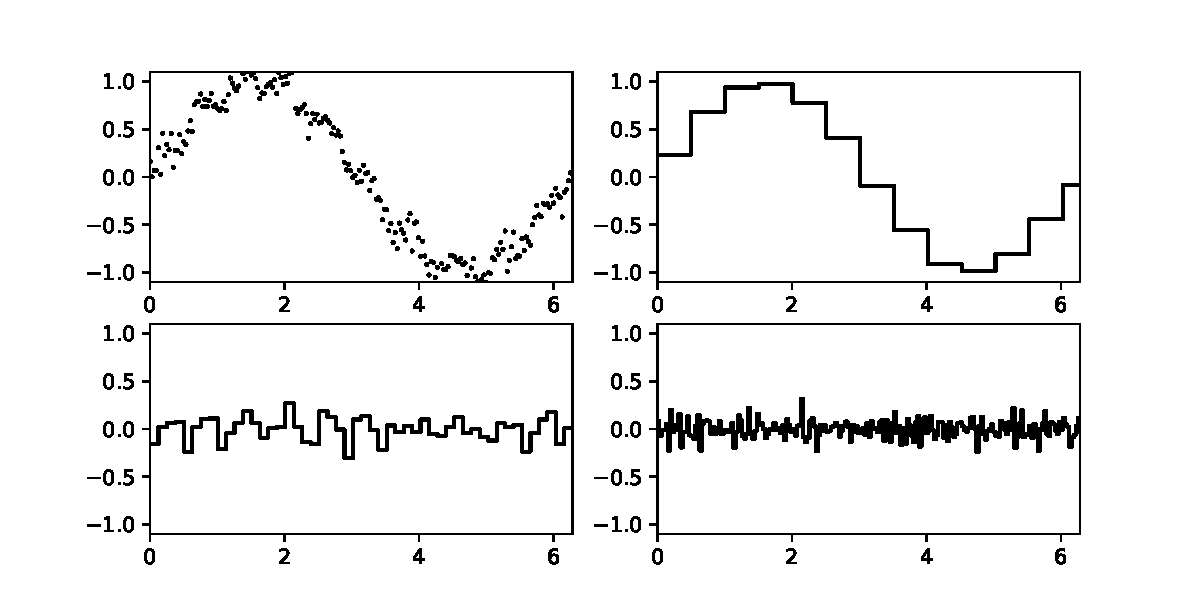
\includegraphics[width=\textwidth]{plots/wavelet}
  \caption{Diskrete Wavelettransformation von 200 diskreten
    Datenpunkten, die analog zu Abbildung~\ref{fig:fouriersin} zwischen
    0 und $2\pi$ als $\sin(x) + 0,1\,sin(10 x) + \xi$ erzeugt
    wurden. Für die Transformation wurden die Wavelets von $(0,1]$ auf
    den Bereich $(0,2\pi]$ gestreckt. Der linke obere Graph zeigt
    nochmals das Ausgangssignal, von rechts oben nach rechts unten
    folgen die Anteile der Stufen 0--3, also $(f,\phi_0)\phi_0 +
    \sum_{j=0}^{3} \sum_{k=0}^{2^j-1} (f,\psi_{jk})\psi_{jk}$, dann
    Stufen 4 und 5 ($\sum_{j=4}^{5} \sum_{k=0}^{2^j-1}
    (f,\psi_{jk})\psi_{jk}$) und schließlich Stufen 6--8, womit die
    Auflösung der Ausgangsdaten erreicht ist.}
  \label{fig:dwt}
\end{figure}

Anders als bei der Fouriertransformation, die eine Zerlegung in
trigonometrische Funktionen darstellt, gibt es für die MSA
verschiedene Sätze von Basisfunktionen mit verschiedenen Eigenschaften
wie Differenzierbarkeit und Lokalität. Im folgenden soll die MSA mit
Hilfe des Haar-Wavelets dargestellt werden, dass das einfachste und
älteste bekannte Wavelet ist. Zunächst betrachten wir die
\emph{Skalierungsfunktion}
\begin{equation}
  \phi(x) = \chi_{(0,1]} =
  \begin{cases}
    1 &\text{für}\; 0 < x \le 1\\
    0 &\text{sonst}
  \end{cases}
\end{equation}
sowie das Haar-\emph{Wavelet}
\begin{equation}
  \psi(x) =
  \begin{cases}
    -1 &\text{für}\; 0 < x \le \frac{1}{2}\\
    1 &\text{für}\; \frac{1}{2} < x \le 1 \\
    0 &\text{sonst},
  \end{cases}
\end{equation}
aus denen wir die Basisfunktionen $\phi_k(x) := \phi(x - k)$ der nullten
Stufe und $\psi_{jk}(x) := 2^{j/2}\psi(2^jx-k)$ der $j$-ten Stufe
konstruieren. Durch die Skalierung mit $2^j$ werden die $\psi_{j,k}$
also immer schmaler, sind aber wegen des Vorfaktors alle normiert,
d.h. $\lVert \psi_{jk} \rVert = 1$. Ebenso sind auch die $\phi_k$
normiert. Zusätzlich sind sämtliche Basisfunktionen zu einander
orthogonal, wie man sich leicht überlegt. Daher lässt sich jede
quadratintegrable Funktion $f$ wie folgt zerlegen:
\begin{equation}
  f(x) = \sum_{k\in\ZZ} (f,\phi_k)\phi_k + \sum_{j\in\NN_0}
  \sum_{k\in\ZZ} (f,\psi_{jk})\psi_{jk}
\end{equation}
Dies ist die Multiskalenanalyse von $f$. Die Koeffizienten der Stufe
$j$ werden auch Details der Stufe $j$ genannt. In der Praxis ist das
Signal durch endlich viele äquidistante Datenpunkte gegeben, analog
zur diskreten Fouriertransformation. In diesem Fall sind die Summen
endlich, da einerseits der Träger endlich ist und damit nur endlich
viele $(f,\phi_k)\neq 0$, und es andererseits keine Details unterhalb
der Auflösung des Signals gibt. Man skaliert dann die Wavelets und
Skalierungsfunktion so, dass der Abstand der Datenpunkte gerade der
halben Breite des Wavelets auf der feinsten Auflösung entspricht, und
$\phi = \phi_0$ bereits das gesamte Interval überdeckt. Für eine nur
auf $[0,1]$ nichtverschwindende Funktion, deren Werte an $2^N$ Punkten
äquidistanten Punkten bekannt ist, reduziert sich die
Multiskalenanalyse zur \emph{diskreten
  Wavelettransformation}\index{Wavelets>-transformation}
\begin{equation}
  \label{eq:idwt}
  f(x) = (f,\phi)\phi +
  \sum_{j=0}^{N-1} \sum_{k=0}^{2^j-1} (f,\psi_{jk})\psi_{jk}.
\end{equation}
Die Anzahl der Koeffizienten ist dann $1 + 1 + 2 + \cdots + 2^{N-1} =
2^N$, also genau die Anzahl der Eingabedaten. Genau wie die diskrete
Fouriertransformation bildet die Wavelettransformation $2^N$ Werte
$f(k/2^N)$ auf $2^N$ Werte $(f,\phi)$ und $(f,\psi_{jk})$ ab und
besitzt eine exakte Rücktransformation, \eqref{eq:idwt}.

Analog zur schnellen Fouriertransformation gibt es auch eine schnelle
Wavelettransformation (FWT), die sogar linearen Aufwand hat, also $\O(N)$
Schritte bei $N$ Datenpunkten benötigt. Eine einfache Implementation
der FWT und der inversen FWT für das Haar-Wavelet zeigt
Codebeispiel~\ref{lst:dwt}. Der Kern dieser Transformation liegt
darin, die Transformierte von der höchsten Detailauflösung herab
aufzubauen, und dadurch die die Integrale approximierenden Summen
schrittweise aufzubauen (\emph{Downsampling}). Für genauere
Informationen siehe zum Beispiel \textcite{daubechies92a}.

Abbildung~\ref{fig:dwt} zeigt einige Detailstufen der
Wavelet-Zerlegung der verrauschten Sinusfunktionen analog
Abbildung~\ref{fig:fouriersin}. Auch hier lässt sich das Rauschen auf
den höheren Detailstufen gut vom Nutzsignal trennen, allerdings kann
die Oberschwingung nicht detektiert werden. Das hängt allerdings vor
allem daran, dass das Haar-Wavelet nicht sehr geeignet ist, da es
nicht glatt ist, im Gegensatz zum Nutzsignal. Daher sind in den
meisten Fällen glatte Wavelets besser geeignet. Das bekannteste
Beispiel von glatten Wavelets sind die Daubechies-Wavelets, die
daneben auch einen kompakten Träger haben, also stark lokalisiert
sind. Mit solchen Wavelets lassen sich sogar reale Musikdaten in
Akkorde zurücktransformieren. Auch der JPEG-Nachfolger JPEG2000
basiert auf einer Wavelettransformation statt einer
Cosinustransformation, allerdings mit
Cohen-Daubechies-Feauveau-Wavelets.

\lstinputlisting[style=floating,firstline=10,
caption={Diskrete Wavelettransformation und ihre Inverse als
  Python-Code. Die Länge der Eingabedaten muss eine Zweierpotenz $2^N$
  sein. Die Details sind in einem Vektor $c$ gespeichert, in der Form
  $c=((f,\phi_0)$, $(f, \psi_{00})$, $(f, \psi_{10})$, $(f, \psi_{11})$,
  $(f, \psi_{20})$, $(f, \psi_{21})$, $(f, \psi_{22}), \ldots,
  (f, \psi_{N-1,2^{N-1}-1}))$.
},
label=lst:dwt]{dwt.py}

%%% Local Variables: 
%%% mode: latex
%%% TeX-master: "padc"
%%% TeX-PDF-mode: t
%%% End: 

% Dies ist Teil der Vorlesung Physik auf dem Computer, SS 2012,
% Axel Arnold, Universitaet Stuttgart.
% 
% Dieses Werk ist unter einer Creative Commons-Lizenz vom Typ
% Namensnennung-Weitergabe unter gleichen Bedingungen 3.0 Deutschland
% zugänglich. Um eine Kopie dieser Lizenz einzusehen, konsultieren Sie
% http://creativecommons.org/licenses/by-sa/3.0/de/ oder wenden Sie sich
% schriftlich an Creative Commons, 444 Castro Street, Suite 900, Mountain
% View, California, 94041, USA.

\chapter{Datenanalyse und Signalverarbeitung}

In diesem Kapitel geht es darum, was man mit einem gemessenen Signal
machen kann und muss. Ein gemessenes Signal kann dabei entweder
tatsächlich von einem Messgerät kommen oder aber das Ergebnis einer
Computersimulation sein. Zwei Fragen sind dabei vor allem wichtig:
Welche Eigenschaften hat das Signal, und wie vertrauenswürdig sind die
Werte?

Um die Eigenschaften von Signalen zu untersuchen, ist die
kontinuierliche Fourieranalyse ein gutes Werkzeug, die das Signal vom
Zeit- in den Frequenzraum überträgt. So lassen sich zum Bespiel
charakteristische Frequenzen und damit Zeitskalen bestimmen. Außerdem
bietet der Übergang in den Frequenzraum analytisch viele Vorteile, die
sich auch auf dem Computer nutzen lassen. So werden zum Beispiel
langreichweitige Wechselwirkungen in Molekulardynamiksimulationen
meist im Frequenzraum berechnet.

Als weiteres Werkzeug werden wir Faltungen kennen lernen, die
erlauben, Signale nach bestimmten Frequenzen zu filtern oder aber aus
der (gemessenen) Antwort eines linearen Systems auf ein einfaches
Eingangssignal die Antwort auf beliebige Signale zu berechnen.

Sollen Signale mit dem Computer weiterverarbeitet werden, müssen diese
\emph{digitalisiert} werden, also in eine Reihe von Zahlen
übersetzt. Üblicherweise passiert dies dadurch, dass das Signal nur zu
äquidistanten Zeitpunkten ausgewertet, \emph{abgetastet} wird. Das
wirft die Frage auf, welche Funktionen dadurch überhaupt gut gemessen
werden können. Wie wir sehen werden, beschränkt diese Abtastung die
Frequenzen, die von einer digitalen Auswertung erfasst werden können.

Die meisten Signale sind außerdem, durch Messungenauigkeiten und
prinzipielle stochastische Prozesse, selbst \emph{stochastisch},
\dh die Verteilung der Ergebnisse vieler Messungen ist
vorherbestimmbar, die einzelne Messung hingegen nicht. Trotzdem sind
Messungen oft korreliert, zum Beispiel weil eine Observable sich nur
kontinuierlich ändert.  Durch Korrelationsanalysen lässt sich
bestimmen, wann Messungen wirklich unabhängig sind. Dies gibt wiederum
Aufschluss über die Zeitskalen wichtiger Prozesse im System, ist aber
auch wichtig für eine korrekte Abschätzung des Messfehlers, womit sich
der letzte Abschnitt beschäftigt.

\section{Kontinuierliche Fouriertransformation}
\index{Fouriertransformation>kontinuierliche}

Für die Analyse zeitlich veränderlicher Signale besonders nützlich ist
die Fouriertransformation, die ein kontinuierliches Signal in den
Frequenzraum übersetzt. Dies gilt nicht nur für periodische Signale,
sondern zum Beispiel auch dann, wenn die Antwort eines Systems auf ein
komplexes Eingangssignal gefragt ist. Der tiefere Grund dafür ist,
dass die Fouriertransformation Differential- und Integraloperatoren in
einfache algebraische Operationen übersetzt.

Betrachten wir nochmals die Fourierreihe im Interval $[-T/2,T/2)$
\begin{multline}
  f(t) = \sum_{n\in\ZZ}
  \left(\frac{\Delta\omega}{2\pi}\int_{-T/2}^{T/2}
    f(t)e^{-i n\Delta\omega t}\, dt\right)
  e^{i n\Delta\omega t}\\
  =
  \frac{1}{\sqrt{2\pi}}\sum_{n\in\ZZ}
  \left(\frac{1}{\sqrt{2\pi}}\int_{-T/2}^{T/2} f(t)e^{-i \omega t}\,dt\right)
  e^{i \omega t}\,\Delta\omega
\end{multline}
mit der Grundfrequenz $\Delta\omega=2\pi/T$ und
$\omega=n\Delta\omega$. Im Grenzwert $T\to\infty$ ergibt sich
\begin{equation}
  \label{eq:contfourierinverse}
  f(t) = \frac{1}{\sqrt{2\pi}}\int_{-\infty}^{\infty}
  \FT(f)(\omega)e^{i \omega t}\,d\omega
\end{equation}
mit
\begin{equation}
  \label{eq:contfourier}
  \FT(f)(\omega) =
  \frac{1}{\sqrt{2\pi}}\int_{-\infty}^{\infty} f(t)e^{-i \omega t}\, dt.
\end{equation}
Die \emph{kontinuierliche Fouriertransformation} $\FT$ ist das
Analogon der periodischen Fourierreihe, ist allerdings keine
Transformation in eine Reihe mehr, sondern eine Abbildung zwischen
Funktionen. Für $\FT$ gelten eine Menge sehr starker Aussagen, die wir
zum großen Teil in ähnlicher Art schon von der Fourierreihe kennen:
\begin{itemize}
\item $\FT(f)$ existiert, falls $f$ quadratintegrabel ist, und
  bildet $f$ auf eine quadratintegrable Funktion ab. Für solche
  Funktionen mit der zugehörigen Norm $\lVert f \rVert_2 =
  \int_{-\infty}^{\infty} \lvert f(t) \rvert^2\,dt$ gilt dann sogar
  die Isometrie
  (\emph{Parsevaltheorem}\index{Parsevaltheorem>kontinuierliches}):
  \begin{equation}
    \lVert \FT(f) \rVert_2 = \lVert f \rVert_2
  \end{equation}
\item $\FT$ ist linear, \dh $\FT(f + \lambda g) = \FT{f} + \lambda
  \FT{g}$.
\item $\FT$ ist reziprok gegen Streckungen, \dh
  \begin{equation}
    \label{eq:fourierreziprok}
    \FT[f(\alpha
    t)](\omega) = \frac{1}{\lvert \alpha \rvert}
    \FT(f)\left(\frac{\omega}{\alpha}\right).
  \end{equation}
  Wird also eine Funktion $\alpha$ immer stärker gestaucht, so wird
  ihre Transformierte immer weiter gestreckt.  Entsprechend wird aus
  Zeitumkehr Frequenzumkehr: $\FT(f(-t))(\omega) = \FT(f)(-\omega)$.
\item $\FT$ ist invertierbar, die Umkehrfunktion $\FT^{-1}$ ist durch
  \eqref{eq:contfourierinverse} explizit gegeben. Offenbar ist auch
  die Umkehrung eine Isometrie, es gilt $\lVert \FT^{-1}(f)
  \rVert_2 =\lVert f \rVert_2$.
\item Weiter gilt $\FT(\FT(f(t))) = f(-t)$, und damit $\FT^4(f) =
  f$. Insbesondere ist auch $\FT^{-1} = \FT^3$. Die
  Fouriertransformation ist damit eine vierte Einheitswurzel auf dem
  Raum der quadratintegrablen Funktionen, ähnlich wie $i$ bei den
  komplexen Zahlen.
\item Eine zeitliche Verschiebung wird zu einer Frequenzmodulation und
  umgekehrt:
  \begin{eqnarray}
    \label{eq:fouriertimeshift}
    \FT(f(t-t_0))(\omega) = e^{-i\omega t_0} \FT(f(t))(\omega)\\
    \label{eq:fourierfreqshift}
    \FT(e^{i\omega_0 t}f(t))(\omega) = \FT(f(t))(\omega-\omega_0).
  \end{eqnarray}
  Wird also ein niederfrequentes Signal (Radioprogramm) auf ein
  hochfrequentes Trägersignal aufmoduliert, verschiebt sich nur dessen
  Spektrum. 
\item Aus der Linearität folgt, dass stets gilt:
  $\FT(\overline{f})(\omega) = \overline{\FT(f)(\omega)}$.
\item Ist Funktion $f$ gerade (symmetrisch), also $f(t) = f(-t)$, so ist
  $\FT(f)(-\omega) = \FT(f)(\omega)$, also gerade (symmetrisch).
\item Ist Funktion $f$ ungerade (antisymmetrisch), also $f(t) = -f(-t)$, so ist
  $\FT(f)(-\omega) = -\FT(f)(\omega)$, ungerade (antisymmetrisch).
\item Ist Funktion $f$ reellwertig, also $f(t) = \overline{f(t)}$, so
  ist $\FT(f)(-\omega) = \overline{\FT(f)(\omega)}$, aber im
  allgemeinen komplexwertig!
\item Für die Fouriertransformierte der Ableitung gilt
  \begin{equation}
    \begin{split}
      \FT\left(\frac{d}{dt}f(t)\right)(\omega) &=
      \frac{1}{\sqrt{2\pi}}\int_{-\infty}^{\infty}
      \left[\frac{df}{dt}(t)\right]e^{-i
        \omega t}\, dt\\
      &\substack{=\\\text{part. Int.}} -\frac{1}{\sqrt{2\pi}}\int_{-\infty}^{\infty}
      f(t)\frac{d}{dt}e^{-i \omega t}\, dt = i\omega
      \FT(f(t))(\omega).
    \end{split}
  \end{equation}
  Dies spielt eine wichtige Rolle beim Lösen von
  Differenzialgleichungen, weil diese in gewöhnliche algebraische
  Gleichungen übergehen.
\item Es gilt die Poissonsche Summenformel
  \begin{equation}
    \label{eq:poissonsumme}
    \sum_{k\in\ZZ}f(t_0 + k\, \delta)=
    \frac{\sqrt{2\pi}}{|\delta|}\sum_{n\in\ZZ}\FT(f)
    \left(\frac{2\pi n}{\delta}\right)
    \exp\left(i \frac{2\pi n}{\delta} t_0\right).
  \end{equation}
  Diese Gleichung beruht darauf, dass $\sum_{t\in\ZZ}f(\cdot + t\,
  \delta)$ eine $\delta$-periodische Funktion ist, die durch eine
  Fourierreihe dargestellt werden kann. Wegen
  \eqref{eq:fouriertimeshift} reicht es
  dabei o.B.d.A. $\delta=1$ zu
  betrachten:
  \begin{multline}
    \sum_{k\in\ZZ}f(t_0 + k) =
    \sum_{n\in\ZZ} \int_0^1 \sum_{k\in\ZZ}f(\tau + k)e^{-2\pi i
      n \tau}\, d\tau
    \, e^{2\pi i n t_0} =\\
    \sum_{n\in\ZZ} \int_{-\infty}^\infty f(\tau)e^{-2\pi i
      n \tau}\, d\tau
    \, e^{2\pi i n t_0}
    = \sqrt{2\pi}\sum_{n\in\ZZ}\FT(f)(2\pi n)\, e^{2\pi i n t_0}.
  \end{multline}

  Eine wichtige Anwendung der Poissonschen Summenformel ist die
  Summation schlecht konvergenter Reihen. Fällt die Funktion $f$ sehr
  langsam gegen unendlich ab, so fällt ihre Fouriertransformierte
  wegen der Reziprozität \eqref{eq:fourierreziprok} im Allgemeinen
  schneller, so das aus einer langsam eine rasch konvergierende Reihe
  wird.
\end{itemize}

\subsection{Spezielle Fouriertransformierte}

Die Fouriertransformierte einer Gaußglocke ist
\begin{equation}
  \FT\left(\frac{1}{\sqrt{2\pi}}e^{-t^2/2}\right)
  =
  \frac{1}{2\pi}e^{-\omega^2/2}\int_{-\infty}^{\infty} e^{-(t-i\omega)^2/2}\, dt
  =
  \frac{1}{\sqrt{2\pi}}e^{-\omega^2/2}
\end{equation}
Die Gaussglocke ist also eine Eigenfunktion der Fouriertransformation
zum Eigenwert 1. Die Fouriertransformation hat tatsächlich sehr viel
mehr echt verschiedene Eigenfunktionen, die Familie der
Hermitefunktionen~\cite{pinsky02a}. Wegen $\FT^4=1$ kann die
Fouriertransformation nur die vier Eigenwerte $\pm 1$ und $\pm i$
haben. Jeder dieser Eigenwerte ist stark degeneriert, also der
Eigenraum zu jedem Eigenwert unendlichdimensional.

Die (formale) Fouriertransformierte der $\delta$-Funktion ist
\begin{equation}
  \label{eq:fourierdelta}
  \FT(\delta(t))(\omega)
  =
  \frac{1}{\sqrt{2\pi}}\int_{-\infty}^{\infty}
  \delta(t)e^{-i \omega t}\, dt = \frac{1}{\sqrt{2\pi}},
\end{equation}
also einfach die konstante Funktion $1/\sqrt{2\pi}$, die ebensowenig
wie die $\delta$-Funktion eine quadratintegrable Funktion
ist. Alternativ lässt sich die Beziehung aus der
Fouriertransformierten der Gaußglocke mit sinkender Varianz herleiten.

\subsection{Numerische kontinuierliche Fouriertransformation}
\label{sec:contdft}

Um die Eigenschaften der kontinuierlichen Fouriertransformation
numerisch zu nutzen, machen wir den Grenzübergang $T\to\infty$
rückgängig und ziehen uns auf ein für die betrachtetete Funktion
hinreichend großes $T$ zurück, so dass $\int_{\lvert t\rvert>T}\lvert
f(t)\rvert^2\, dt$ hinreichend klein ist. Das geht insbesondere, wenn
das Signal endlichen Träger hat, wie das bei echten gemessenen
Signalen stets der Fall ist.

Wir betrachten nun als Signal eine Funktion $f$, die wir nur an auf
einem äquidistanten Gitter $t_k = t_0 + k\frac{T}{N}$, $k=0(1)N-1$
kennen, also im Intervall $[t_0, t_o + T]$. Dann setzen wir
$\omega_0:=\frac{2\pi}{T}$ und $\Delta := \frac{T}{N}$, und erhalten
für ganzzahliges $n$
\begin{multline}
  \label{eq:dftcont}
  \FT(f)(\omega_0 n)\approx
  \frac{1}{\sqrt{2\pi}}\int_{t_0}^{t_0 + T} f(t)e^{-i n \omega_0 t}\, dt
  \approx
  \frac{1}{\sqrt{2\pi}}\sum_{k=0}^{N-1}
  \Delta f(t_k)
  e^{-i n\omega_0 \left(t_0 + k\Delta\right)}\,
  \\
  =   \Delta \frac{e^{-i n\omega_0 t_0}}{\sqrt{2\pi}}\sum_{k=0}^{N-1}
  f(t_k) e^{-2\pi i n k / N}\,
  =\frac{T}{N}\frac{\left(e^{-i\omega_0 t_0}\right)^n}{\sqrt{2\pi}} \text{DFT}(f(t_k))_n\,,
\end{multline}
wobei DFT die diskrete Fouriertransformation aus \eqref{eq:dft}
bezeichnet. Meist werden Messungen bei $t=0$ begonnen, die Funktion
ist dann nur im positiven Halbinterval von Null verschieden.  In
diesem Fall wählt man natürlicherweise $t_0 = 0$, so dass der Faktor
$e^{-i\omega_0 t_0} = 1$ entfällt. Wir werden allerdings später noch
Faltungen kennenlernen, bei denen es häufig natürlicher ist, eine
symmetrische Lage der Filterfunktion um die Null anzunehmen. In diesem
Fall wählt man $t_0 = -T/2$, so dass $e^{-i\omega_0 t_0} = -1$.

Die Koeffizienten der DFT sind periodisch, daher auch diese Näherung
für $\FT(f)$. Tatsächlich sollten die Koeffizienten aber nur als
Frequenzen im Interval $[-\omega_0 N/2,\omega_0 N/2]$ interpretiert
werden, alle Frequenzen außerhalb dieses Intervals sollten als Null
angesehen werden. Der Grund dafür ist das Abtasttheorem, dass im
folgenden Abschnitt besprochen wird. Dieses besagt, dass bei einem
Zeitschritt $\Delta=T/N$ nur Kreisfrequenzen bis $\omega_0 N/2 =
\pi/\Delta$ eindeutig gemessen werden können. Daher ist die
Beschränkung auf das innerste Interval die natürliche
Interpretation. Bei rein reellen Signalen ist es daher günstiger,
direkt die reellen Varianten der FFT-Implementationen zu nutzen, die
von vorneherein nur die relevanten positiven Koeffizienten bis $N/2$
zurückgeben.

Die Einschränkung der Frequenzen ist besonders wichtig, wenn $N$
ungerade ist und die um Null symmetrische Lage von $-T/2$ bis $T/2$
gewählt wird. Dann ist $\left(e^{-i\omega_0 t_0}\right)^{N-n} =
(-1)^{N-n} = - (-1)^{-n} = -\left(e^{-i\omega_0 t_0}\right)^{-n}$. Mit
anderen Worten, wird einfach die gesamte diskrete
Fouriertransformierte mit $(-1)^n$ multipliziert, so bekommen die
negativen Frequenzen das falsche Vorzeichen. Das hat drastische
Konsequenzen: wenn die Ursprungsfunktion reell ist, gilt
$DFT(f_k)_{-n}=\overline{DFT(f_k)}_{n}$, für die genäherte
kontinuierliche Fouriertransformierte also
$\FT(f)(-\omega)=-\overline{\FT(f)(\omega)}$. Das entspricht der
Tranformierten einer rein imaginären Funktion!

Analog wie die Fouriertransformation selber lässt sich auch ihre
Rücktransformation nähern:
\begin{equation}
  \label{eq:idftcont}
  \FT^{-1}(f)(t_k)\approx
  \text{iDFT}\left(\sqrt{2\pi}\frac{N}{T}\left(e^{i\omega_0 t_0}\right)^n f_n\right)_k
\end{equation}
Der Faktor $\left(e^{i\omega_0 t_0}\right)^n$ invertiert genau den
Faktor $\left(e^{-i\omega_0 t_0}\right)^n$ der
Vorwärtstransformation. Für $t_0=0$ ist er wieder 1 und muss nicht
berücksichtigt werden, bei $t_0=-T/2$ ist er $(-1)^n$.

Die bekannten schnellen FFT-Routinen lassen sich also auch für die
numerische Bearbeitung der kontinuierlichen Fouriertransformation
nutzen. Auf diese Weise ist \zb Abbildung~\ref{fig:fourierfaltung}
entstanden.

\subsection{\keyword{Abtasttheorem}}

In der Praxis sind Signale meist als diskrete Werte an (endlich
vielen) äquidistanten Stellen beziehungsweise Zeitpunkten gegeben, zum
Beispiel, weil ein Messgerät Daten in regelmäßigen Abständen liefert.
Eine wichtige Frage ist, wie gut man das reale Signal und sein
Frequenzspektrum aus den diskreten Datenpunkten rekonstruieren kann.

Hierzu betrachten wir zunächst ein \emph{bandbreitenbeschränktes
  Signal} $f$, \dh ein Signal, dessen Fouriertransformierte einen
kompakten Träger $[-\omega_\text{max},\omega_\text{max}]$ hat. Dann besagt die
Poissonsche Summenformel~\eqref{eq:poissonsumme}, dass für
$\omega\in[-\omega_\text{max},\omega_\text{max}]$
\begin{equation}
  \FT(f)(\omega) =
  \sum_{k\in\ZZ}\FT(e^{-i\omega \cdot} f)\left(2k\omega_0\right)
  =
  \frac{1}{\sqrt{2\pi}}
  \sum_{n\in\ZZ} e^{-i \omega n \Delta}f\left(n \Delta\right)
\end{equation}
mit $\Delta=\pi/\omega_\text{max}$. Die Fouriertransformierte eines
bandbreitenbeschränkten Signals lässt sich also \emph{exakt} nur aus
den Funktionswerten an den äquidistanten diskreten Stellen mit
Abtastrate $\Delta$ berechnen. Dadurch kann natürlich auch die
Funktion exakt aus ihrer Fouriertransformierten rekonstruiert werden:
\begin{equation}
  \label{eq:ftreconst}
  f(t)
  = \frac{\Delta}{2\pi}\sum_{n\in\ZZ} f\left(n \Delta\right)
  \int_{-\omega_\text{max}}^{\omega_\text{max}} e^{-i \omega (t - n\Delta)} \,d\omega
  = \frac{\Delta}{\pi}\sum_{n\in\ZZ} f\left(n \Delta\right)
  \frac{\sin(\omega_\text{max}(t-n\Delta))}{t-n\Delta}.
\end{equation}

Ist nun umgekehrt ein Signal $f$ an äquidistanten diskreten Stellen
$n\Delta$ gegeben, so lässt sich diesem gemäß \eqref{eq:ftreconst} ein
kontinuierliches Signal zuordnen, dessen Fouriertransformierte nur in
$[-\omega_\text{max},\omega_\text{max}]$ nicht verschwindet, wobei $\omega_\text{max} =
\pi/\Delta$. Das bedeutet, dass bei Abtastrate $\Delta$ nur Frequenzen
bis zur Nyquist-Frequenz $f_\text{Nyquist}=\frac{1}{2\Delta} =
\frac{\omega_\text{max}}{2\pi}$ eindeutig abgetastet werden können, ähnlich wie
im periodischen Fall.

\section{Faltungen}
\index{Faltung}

Die \emph{Faltung} der quadratintegrablen Funktionen $f$ und $g$ ist
definiert als
\begin{equation}
  (f \star g)(t) := \int_{-\infty}^{\infty} f(t')g(t-t')\,dt'.
\end{equation}
Das negative Vorzeichen von $t'$ in der zweiten Funktion sorgt
dafür, dass die Faltung kommutativ ist. Weitere Eigenschaften der
Faltung sind Linearität in den Komponenten und sogar
Assoziativität. Die Faltung verhält sich also so ähnlich wie die
klassische Multiplikation und wird daher mit dem Zeichen $\star$
bezeichnet.  Vereinfacht gesagt, deponiert die Faltung an jedem Punkt
$t$ die Funktion $f$, skaliert mit $g(\cdot - t) $. Daher ist \zb
\begin{equation}
  (\delta(\cdot - t_0) \star g)(t) = g(t - t_0).
\end{equation}
\index{Glättung}
Wird nun statt der unendlich dünnen $\delta$-Funktion zum Beispiel
eine Gaußglocke gewählt, so wird die Funktion $g$ verschmiert
bzw.\ geglättet, siehe Abbildung~\ref{fig:fourierfaltung}.

\begin{figure}
  \centering
  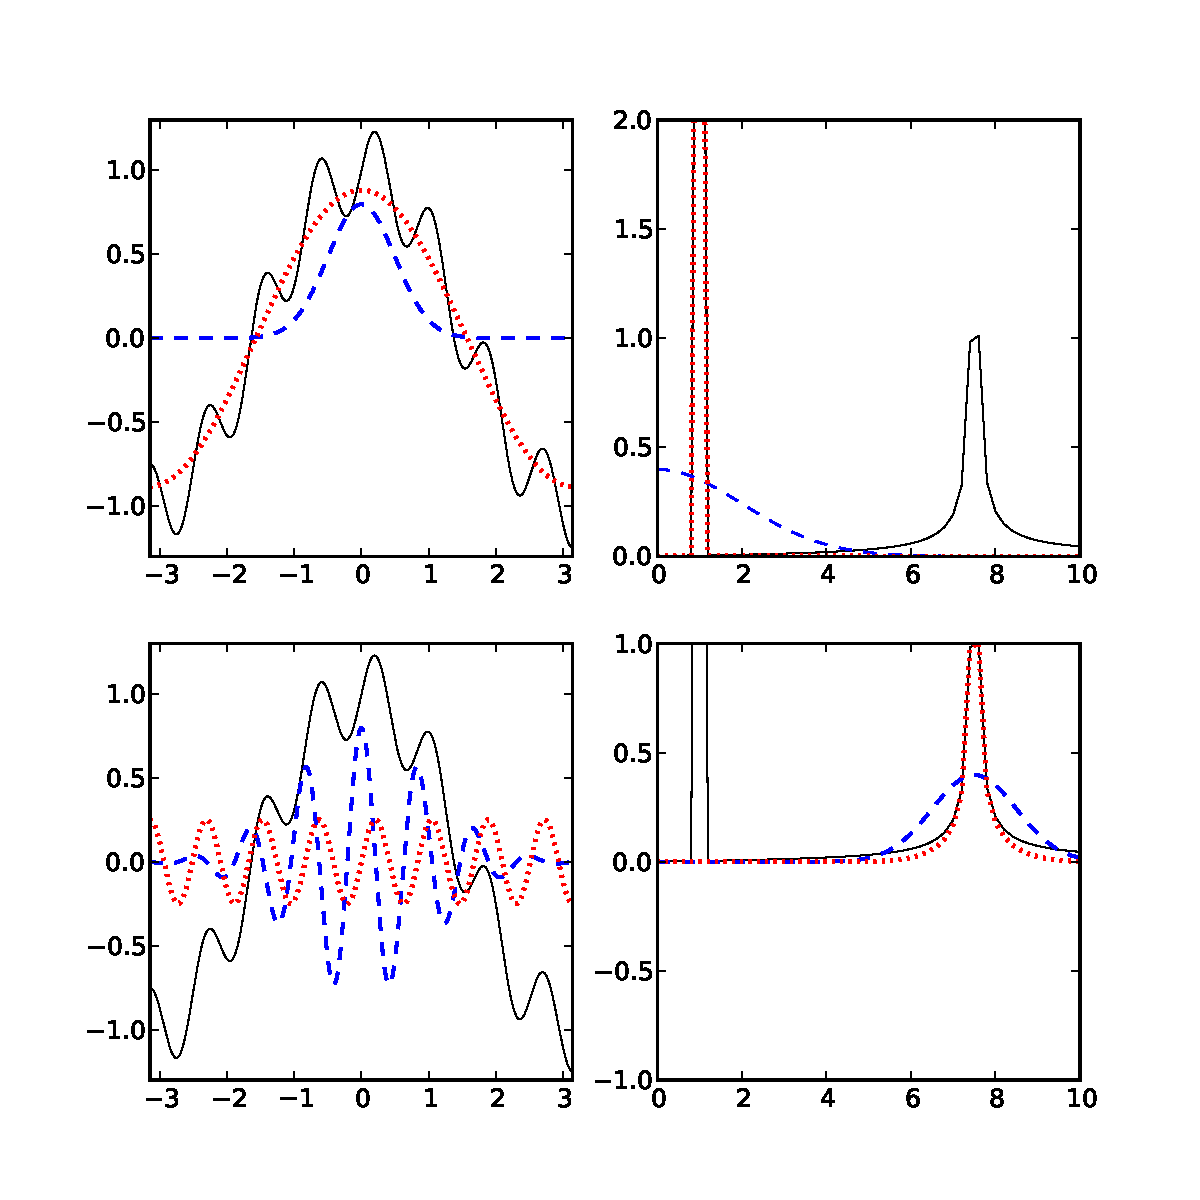
\includegraphics[width=\textwidth]{plots/fouriertrafo}
  \caption{Oben links: Summe zweier Schwingungen $\cos(x) +
    0,25\sin(7,5 x)$ (schwarze Linie), die mit einer Gaußglocke (blau
    gestrichelt) gefaltet wird. Das Ergebnis (rote gepunktete Linie)
    ist die quasi ungestörte langsame Schwingung ohne die
    höherfrequente Schwingung, die weggeglättet wurde. Oben rechts:
    Fouriertransformierte der Funktionen. Klar sichtbar ist die
    hochfrequente Störung mit einer Frequenz von $7,5$, die im
    gefilterten Signal fehlt. In der unteren Reihe wurde eine
    frequenzverschobene Gaußglocke benutzt, um statt der langsamen die
    schnelle Schwingung zu filtern; die Farbcodierung ist wie
    oben. Gemäß \eqref{eq:fourierfreqshift} bewirkt die
    Frequenzverschiebung eine Modulation der Gaußfunktion.}
  \label{fig:fourierfaltung}
\end{figure}

Die Fouriertransformierte der Faltung zweier Funktionen ist
\begin{equation}
  \label{eq:fourierfaltung}
  \begin{split}
    \FT(f\star g)(\omega) &=
    \frac{1}{\sqrt{2\pi}}\int_{-\infty}^{\infty}
    \int_{-\infty}^{\infty} f(t')g(t-t')\,dt' e^{-i \omega t}\,
    dt\\
    &= \frac{1}{\sqrt{2\pi}}\int_{-\infty}^{\infty}
    \int_{-\infty}^{\infty} f(t') g(t) e^{-i \omega (t+t')}\, dt\,
    dt'\\
    &= \frac{1}{\sqrt{2\pi}} \int_{-\infty}^{\infty} f(t')e^{-i
      \omega t'}\, dt' \int_{-\infty}^{\infty} g(t) e^{-i \omega
      t}\, dt = \sqrt{2\pi}\FT(f)(\omega)\FT(g)(\omega).
  \end{split}
\end{equation}
Die Faltung geht also in eine punktweise Multiplikation über. Im
Fourierraum lässt sich also sehr viel schneller falten, als im
Realraum, wo ja für jeden Punkt ein Integral zu lösen ist.

Dies nutzt man auch numerisch, um Faltungen zu berechnen, in
Verbindung mit \eqref{eq:dftcont}. Seien zwei Sätze mit $N$ Datenpunkten $f_k =
f(t_k)$  mit $t_k = t_0 + k\frac{T}{N}$  und $g_k = g(t'_k) $ mit
$t'_k = t'_0 + k\frac{T}{N}$ gegeben. Mit anderen Worten, die beiden
Funktionen müssen mit der selben Frequenz abgetastet worden sein, der
Anfangszeitpunkt kann aber verschieden sein. Das ist etwa beim
Glätten wichtig, bei dem die Filterfunktion meist symmetrisch um die
Null definiert ist, die zu glättende Funktion aber beliebig liegen
kann. Es gilt
\begin{multline}
  \label{eq:discretefold}
  (f\star g)(t_k) =
  \sqrt{2\pi}\FT^{-1}\left(\FT(f)(\omega)\FT(g)(\omega)\right)(t_k)\\
  \approx
  iDFT\left(2\pi \frac{N}{T} \left(e^{i\omega_0 t_0}\right)^n
  \left[\frac{T^2}{2\pi N^2}\left(e^{-i\omega_0 t_0}\right)^n\text{DFT}(f_k)_n\left(e^{-i\omega_0 t'_0}\right)^n\text{DFT}(g_k)_n\right]\right)_k\\
  =
  \frac{T}{N} \text{iDFT}\left[\left(e^{-i\omega_0 t'_0}\right)^n DFT(f_k)_n DFT(g_k)_n\right]_k.
\end{multline}
Wie im Abschnitt~\ref{sec:contdft} besprochen, muss $n$ als Frequenz
im Bereich $-N/2$ bis $N/2$ interpretiert werden. Man beachte, dass
der Faktor $\left(e^{-i\omega_0 t'_0}\right)^n$ nur durch den Aufpunkt
$t'_0$ der Abtastung der Funktion $g$ bestimmt ist, da wir an den
Stellen $t_k$ auswerten. Dadurch ist die Funktion $g$ die
Filterfunktion, die auf $f$ angewendet wird. Ist $g$ wie üblich
symmetrisch um Null abgetastet, so ist $\left(e^{-i\omega_0
    t'_0}\right)^n=(-1)^n$. Vergisst man diesen Term, entspricht das
einem impliziten Verschieben der Filterfunktion zur Null hin.
Die Lage $t_0$ der Abtastung der Funktion $f$ kann hingegen beliebig
verschoben sein. Die Faltung wird in jedem Fall natürlich nur im
Abtastbereich der Funktion $f$ berechnet.

\subsection{Filter}
\index{Filter}

Außerdem lässt \eqref{eq:fourierfaltung} noch eine weitere
Interpretation der Faltung der Funktion $g$ mit der Funktion $f$ zu:
Ist $f$ bzw. $\FT(f)$ reellwertig und symmetrisch, so werden die
einzelnen Frequenzkomponenten der Funktion $g$ mit den
Frequenzanteilen von $f$ gestreckt bzw.\ gestaucht, $g$ also
frequenzgefiltert. Man beachte, dass $g$ für die Definition
\eqref{eq:fourierfaltung} nicht quadratintegrabel sein muss, sofern
der Filter $f$ schnell genug abfällt. Insbesondere kann $g$ eine nur
beschränkte, aber nicht abklingende Funktion sein, wie etwa ein
Messsignal.

Durch Wahl einer symmetrischen und reellwertigen
Fouriertransformierten und Rücktransformation lassen sich also
beliebige Frequenzfilter realisieren; in der Praxis wird natürlich
direkt im Fourierraum gefiltert. Später lernen wir die numerische
diskrete Fouriertransformation kennen, die nicht zuletzt wegen dieser
Filtereigenschaften so wichtig ist. Abbildung~\ref{fig:fourierfaltung}
illustriert einen (gaußschen) Tiefpassfilter und einen Bandfilter, die
nur bestimmte Frequenzen passieren lassen. Daher wird beim
Tiefpassfilter die aufgeprägte hochfrequente Schwingung unterdrückt,
beim Hochpassfilter hingegen die an sich dominante langsame
Schwingung.

\subsection{Antwort zeitinvarianter linearer Systeme}
\index{zeitinvariante lineare Systeme}

Eine weitere wichtige Anwendung der Faltung ist die Bestimmung der
Antwort eines zeitinvarianten linearen Systems auf ein beliebiges
Eingangssignal. Einfach zu messen ist typischerweise die Antwort
$A_\theta(t)$ des Systems auf einen Einschaltvorgang, also ein
Eingangssignal der Form
\begin{equation}
  \theta(t) =
  \begin{cases}
    0 & \text{für}\; t < 0\\
    1 & \text{für}\; t \ge 0.
  \end{cases}
\end{equation}
Um daraus die Antwort auf ein beliebiges Eingangssignal zu bestimmen,
schreiben wir das Eingangssignal $f$ als $f = f \star \delta$. Wegen
der Linearität der Faltung und der Systemantwort ist die Antwort auf
das Signal $f$ gegeben durch die Faltung $A_f(t) = f \star A_\delta$
mit der Antwort auf einen $\delta$-Impuls. Diese Antwort wiederum
lässt sich aus der Sprungantwort durch einfach Ableitung erhalten, was
mit Hilfe der Fouriertransformierten sehr bequem zu berechnen ist:
\begin{equation}
  A_f(t) = f \star A_\delta = f \star
  \frac{d}{dt} A_\theta = \sqrt{2\pi} \FT^{-1}\bigl( i\omega \FT(f) \FT(A_\theta)\bigr).
\end{equation}

\section{Kreuz- und Autokorrelation}
\index{Korrelationsanalyse}

Bis jetzt haben wir uns mit der Verarbeitung idealer Signale
beschäftigt, die zu einem gegebenen Zeitpunkt einen prinzipiell
eindeutig vorherbestimmten Wert haben.  Reale Signale sind aber oft
verrauscht, entweder durch Messungenauigkeiten, Bauteiltoleranzen oder
prinzipielle stochastische Prozesse.  Trotzdem möchte man oft wissen,
ob zwei gemessene Signale von einander abhängig, \emph{korreliert},
sind. Zum Beispiel könnte man die Position eines Elektrons und seinen
Spin, die Menge der verkauften Eis- und Sonnencreme, oder auch die
Position eines Pendels zu zwei verschiedenen Zeitpunkten betrachten.
In den beiden letzteren Fällen werden diese im Allgemeinen korreliert,
also abhängig, sein. Allerdings gibt dies keinen Aufschluss über den
dahinterstehenden kausalen Mechanismus. Im Fall des Pendels rührt die
Korrelation daher, dass es sich in kurzer Zeit nicht beliebig weit von
seiner Ausgangsposition bewegen kann. Bei der Eis- und Sonnencreme
wird es vermutlich auch eine Korrelation geben, aber weder erzeugt
Eiscreme Sonnenbrand, noch macht Sonnencreme Lust auf Eis. Allerdings
haben wir Menschen nunmal bei strahlendem Sonnenschein mehr Lust auf
Eis, aber brauchen auch Sonnencreme.

Formal betrachten wir zunächst zwei Observablen $A$ und $B$. Diese
beiden heißen genau dann unkorreliert, falls die Mittelwerte
$\mean{A\cdot B} = \mean{A}\mean{B}$
bzw. $\mean{(A-\mean{A})(B-\mean{B})}=0$ erfüllen.  Im Allgemeinen
wird man aber vielleich nicht erwarten, dass sich die Änderung einer
Observablen unmittelbar in einer anderen niederschlägt, sondern erst
nach einer Zeit $\tau$.  Man betrachtet daher die Korrelation zwischen
$A$ und $B$ mit einem zeitlichen Versatz von $\tau$, die
\emph{\keyword{Kreuzkorrelationsfunktion}}:
\begin{equation}
  \label{eq:crosscorr}
  C(A,B)(\tau) := \mean{A(0)B(\tau)},
\end{equation}
wobei die Signale $A$ und $B$ zeitinvariant sein sollen, so dass der
Zeitpunkt $t=0$ beliebig gewählt sein kann. Für große $\tau$
dekorrelieren die Signale, daher gilt $C(A,B)\to \mean{A}\mean{B}$ für
$\tau\to\infty$. Wird stattdessen die normierte Kreuzkorrelation
$C(A-\mean{A}, B-\mean{B})$ betrachtet, verschwindet dieses also im
Limit $\tau\to\infty$.

$\mean{\cdot}$ bezeichnet in der Physik üblicherweise den
Ensemblemittelwert, also den Mittelwert über alle möglichen
Realisationen des Experiments. Sind nun $A=A(t)$ und $B=B(t)$
zeitliche Messreihen eines zeitinvarianten Systems, so ermittelt man
die Mittelwerte üblicherweise als Zeitmittelwerte, also Integrale über
die Zeit:
\begin{equation}
  \label{eq:crosscorrtime}
  C(A,B)(\tau) = \mean{A(0)\cdot B(\tau)} \stackrel{!}{=}
  \lim_{T\to\infty}\frac{1}{T}\int_{-T/2}^{T/2} A(t)B(t+\tau)\,dt.
\end{equation}
Das Ausrufezeichen soll andeuteten, dass dies eine Annahme ist, denn
die Gleichheit gilt nur genau dann, wenn das System \emph{ergodisch}
ist, \dh\,, dass der Prozess bei einer unendlich langen zeitlichen
Messung alle möglichen Realisationen einmal besuchen wird. Diese
Annahme wird meist gemacht, obwohl die Ergodizität für die meisten
Systeme nicht bewiesen werden kann. Hinzu kommt, dass ja in der Praxis
niemals über beliebig lange Zeiträume gemittelt werden kann. Daher
können auch endliche, aber hohe Energiebarrieren zu einem
systematischen Fehler führen, weil das System im Zeitraum der Messung
nur den Teil des Phasenraums besucht, der von der Energiebarriere
eingeschlossen ist, selbst wenn auch andere Bereiche zulässig wären.

$\mean{A}$ bzw. $\mean{B}$ sind oft gar nicht genau bekannt, und
müssen numerisch durch \mbox{(Zeit--)}Mittelung der Daten bestimmt
werden. Da hier aber normalerweise dieselben Daten zugrunde gelegt
werden, die auch zu Berechnung der Kreuzkorrelation selber genutzt
werden, sind diese notwendigerweise korreliert, was zu kleinen
Abweichungen in der Kreuzkorrelationsfunktion führt. Im häufigen Fall,
dass eine Observable aus Symmetriegründen einen Mittelwert von Null
haben muss, sollte daher auf keinen Fall der numerische gemessene
Mittelwert abgezogen werden, "`um das Ergebnis zu verbessern"'. Diese
übliche Praxis ist falsch, da sie ja erzwingt, dass der letzte
Datenpunkt der gemessenen Kreuzkorrelationsfunktion notwendigerweise
auf $\mean{A}\mean{B}$ abfällt, selbst wenn einfach nur das
Messinterval zu kurz gewählt wurde. Daher führt diese Methode zu einer
Unterschätzung der Langzeitkorrelationen!

Analog zu \eqref{eq:crosscorrtime} kann man die Kreuzkorrelation auch
für \emph{endliche} Signale definieren. Für zwei quadratintegrable, reelle
Signale $f$ und $g$ ist in Analogie die Kreuzkorrelationsfunktion
definiert als
\begin{equation}
  C(f,g)(\tau) = \int_{-\infty}^{\infty} f(t)g(t+\tau)\,dt,
\end{equation}
wobei wegen der Quadratintegrabilität auf die Normierung verzichtet
werden kann. Diese Kreuzkorrelation misst keine Korrelationen im
stochastischen Sinne mehr, weil das Integral nun keine Zeitmittelung
mehr darstellt. Stattdessen ist $C(f,g)(\tau)$ in diesem Fall ein Maß
dafür, wie sehr sich die Signale $f$ und $g$ mit einem Zeitversatz
$\tau$ im Verlauf ähneln. Diese Form der Kreuzkorrelation ähnelt einer
Faltung sehr. Tatsächlich ist
\begin{equation}
  C(f,g)(\tau) = \bigl(f \star g(-\cdot)\bigr)(-\tau) =
  \bigl(f(-\cdot) \star g\bigr)(\tau)
\end{equation}
und kann damit effizient im Frequenzraum bestimmt werden:
\begin{equation}
  \label{eq:crosscorrfft}
  C(f,g)(t) = \sqrt{2\pi}\FT^{-1}
  \bigl(\FT(f)(-\omega)\FT(g)(\omega)\bigr) = \sqrt{2\pi}\FT^{-1}
  \bigl(\overline{\FT(f)}\FT(g)\bigr).
\end{equation}

Kommen wir nun zu unserem Ausgangsproblem mit zwei stochastischen,
zeitinvarianten Variablen $A$ und $B$ und dem Zeitmittel zurück. Wie
üblich nehmen wir an, dass $A$ und $B$ an endlich vielen, diskreten
Zeitpunkten $k\Delta$, $k=0(1)N-1$, gemessen wurden. Die Messung
erstreckt sich also über den Zeitraum $[0,T]$ mit $T=N\Delta$. Dann
ist eine Näherung für die Kreuzkorrelation von $A$ und $B$ gegeben
durch
\begin{equation}
  \label{eq:crosscorrnum}
  C(A,B)(k\Delta) = \mean{A(0)\cdot B(k\Delta)}
  \approx
  \frac{1}{N-k}\sum_{l=0}^{N-k}A(l\Delta)B\left((l+k)\Delta\right)
  \quad\text{für}\; k=0(1)N-1.
\end{equation}
Die unterschiedliche Gewichtung $1/(N-k)$ ergibt sich durch die
unterschiedliche Anzahl an Messungen für den Versatz $k$. Für große
Versätze ist die Anzahl der Messungen sehr klein (für $k=N-1$ nur noch
eine), daher muss $k \ll N$ sein. Form \eqref{eq:crosscorrnum} ist
numerisch allerdings nicht sehr effizient auszuwerten, da im
allgemeinen $2N^2$ viele Operationen benötigt werden.  Daher liegt es
nahe, auch hier die FFT gemäß \eqref{eq:discretefold} zur
Beschleunigung einzusetzen.  Für gleich lange Messreihen $A$ und $B$
ergibt sich
\begin{equation}
  \label{eq:crosscorrnumfft}
  C(A,B)(k\Delta)
  \approx
  \frac{1}{N}\,\text{iDFT}
  \bigl(\overline{\text{DFT}(A)}\,\text{DFT}(B)\bigr)(k)\,,
\end{equation}
wobei angenommen wurden, dass beide Messungen bei $t_0=0$ begonnen
haben, so dass der Faktor $\left(e^{-i\omega_0 t_0}\right)^n$
entfällt.

Die Berechnung der 2 DFTs sowie der inversen DFT braucht etwa $6 N\log
N$ Operationen, was normalerweise wesentlich weniger als die $2N^2$
der direkten Berechnung ist.  Allerdings werden das Signal und damit
auch $C(A,B)$ durch die Benutzung der DFT implizit mit Periode
$N\Delta$ periodisiert. Daher sollte $C(A,B)(k\Delta)$ nur für $k\ll
N/2$ interpretiert werden. Wie besprochen gilt dies allerdings genauso
auch für die direkte Auswertung nach \eqref{eq:crosscorrnum}, da für
größere $k$ die Anzahl der Messwerte nicht ausreichend ist.

In Python sieht die Berechnung der Kreuzkorrelation so aus:
\begin{lstlisting}
import numpy
import numpy.fft as fft

def kreuzkorrelation(A, B):
    ftA = fft.fft(A).conj()
    ftB = fft.fft(B)
    return numpy.real(fft.ifft(ftA*ftB))/A.shape[0]
\end{lstlisting}

\begin{figure}
  \centering
  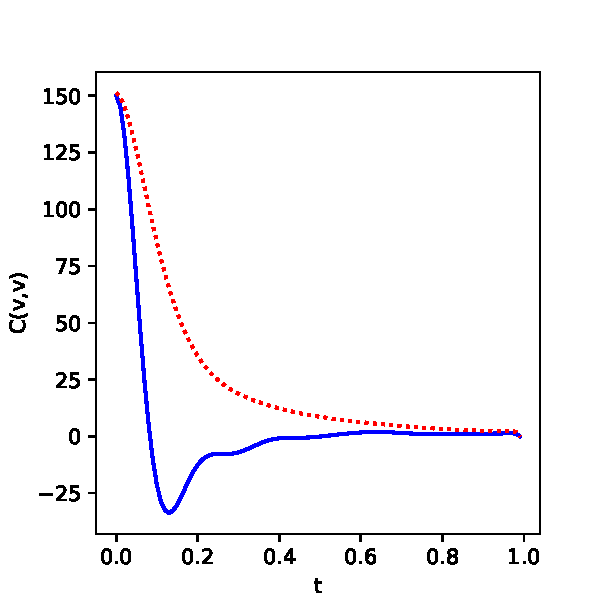
\includegraphics[width=0.5\textwidth]{plots/v_ac}
  \caption{Geschwindigkeitsautokorrelationsfunktion einer temperierten
    Lennard-Jones-Flüs\-sig\-ke\-it mit niedriger Dichte (rot
    gepunktet) und hoher Dichte (blau durchgezogen). Für die niedrige
    Dichte ist die Autokorrelationsfunktion im wesentlichen
    exponentiell abfallend, mit einer Korrelationszeit $\tau_c=0.17$,
    die durch die Kopplungszeit des Thermostaten bestimmt ist.}
  \label{fig:vac}
\end{figure}

\subsection{Autokorrelationsfunktion}

Im Spezialfall $A=B$ spricht man von der
\emph{\keyword{Autokorrelationsfunktion}}. Diese ist offenbar
symmetrisch, daher sind nur Zeitversätze $\tau\ge 0$ von
Interesse. Die Autokorrelationsfunktion misst gewissermaßen, wie lange
es dauert, bis die Observable nicht mehr von ihrem vorherigen Wert
abhängt, wann es diesen sozusagen "`vergisst"'. In dem häufigen Fall,
dass die Autokorrelationsfunktion zunächst exponentiell abfällt, lässt
sich dem Gedächtnis eine Zeitkonstante $\tau_c$, die
\emph{\keyword{Korrelationszeit}}, zuordnen. Diese kann man entweder
durch einen geeigneten Funktionsfit bestimmen, oder aber durch
Integration aus
\begin{equation}
  \label{eq:tauc}
  \int_{0}^{\infty} C(A,A)(\tau)\,d\tau = \int_{0}^{\infty}
  C(A,A)(0)e^{-\tau/\tau_c}\,d\tau = \tau_c\,C(A,A)(0).
\end{equation}

Abbildung~\ref{fig:vac} zeigt die Geschwindigkeitsautokorrelation
$C(v,v)$ einer temperierten Lennard-Jones-Flüs\-sig\-ke\-it bei zwei
verschiedenen Dichten. Die Temperierung wird dabei mit Hilfe eines
Thermostaten erreicht, der die Teilchen stochastisch an ein Wärmebad
koppelt. Dadurch dekorreliert die Geschwindigkeit eines Teilchens in
einer Korrelationszeit von etwa $1/6$.

$C(v,v)$ wird häufig dazu benutzt, um die Diffusionskonstante $D =
\int_0^{\infty} C(v,v)(\tau)\, d\tau$ des Systems zu bestimmen, die
also eng mit der Korrelationszeit des Thermostaten verwandt ist.  Bei
niedriger Dichte ist das System annähernd ein ideales Gas, und die
Teilchen dekorrelieren im wesentlichen nur durch den Einfluss des
Thermostaten, der durch Zufallskräfte wirkt, daher ist $C(v,v)$
tatsächlich gut exponentiell abfallend.  Formel~\eqref{eq:tauc}
bestimmt die Korrelationszeit mit guter Genauigkeit zu etwa
$\tau_c=0.17$, wie durch den Thermostaten zu erwarten. Im Falle der
dichteren Flüssigkeit hingegen kann diese Formel nicht angewendet
werden, da die Autokorrelation kein einfacher exponentieller Abfall
mehr ist, da auch Stoßprozesse eine wichtige Rolle spielen. Diese
führen zum Durchschwingen der Autokorrelationsfunktion.

\section{Messfehlerabschätzung}
\index{Messfehler}

In diesem letzten Abschnitt zur Datenanalyse geht es darum, wie der
Messfehler bei der Messung des Erwartungswerts einer stochastischen
Observable abgeschätzt werden kann. Wir betrachten also eine Messreihe
$x_i$, $i=1(1)N$, die verschiedene Messungen einer stochastischen
Observablen $x$ darstellen, deren Verteilung zeitlich unveränderlich
sein soll (wie zum Beispiel die Temperatur eines abgeschlossenen
Systems im Gleichgewicht). Die gesuchte Größe ist dann meist der
Erwartungswert $\mean{x}$ der Observablen oder ihre \emph{Varianz}
\begin{equation}
  \sigma^2(x) = \mean{\bigl(x-\mean{x}\bigr)^2}
  = \mean{x^2} - 2\mean{\mean{x}x}  + \mean{x}^2
  = \mean{x^2} - \mean{x}^2,
\end{equation}
die die erwartete quadratische Abweichung einer Messung vom
Erwartungswert beschreibt. Sie ist wie der Erwartungswert eine
Eigenschaft der zu messenden Observablen $x$ und im Gegensatz zum
Messfehler nicht von der Anzahl der Messungen abhängig.

Aus der Messreihe lässt sich der Erwartungswert dieser Observablen als
\begin{equation}
  \label{eq:mean}
  \mean{x} \approx \bar{x} := \frac{1}{N}\sum_{i=1}^N x_i
\end{equation}
abschätzen, da $\mean{\bar{x}} = \mean{x}$. Doch was ist nun der
Fehler, den wir mit dieser Schätzung machen? Dieser ist die zu
erwartende quadratische Abweichung des numerischen Mittelwerts vom
tatsächlichen Erwartungswert:
\begin{equation}
  \mean{\left(\overline{x} - \mean{x}\right)^2} =
  \frac{1}{N^2}\sum_{i,j=1}^N \mean{x_ix_j} -
  \frac{2}{N}\sum_{i=1}^N \mean{x_i}\mean{x} + \mean{x}^2
  = \frac{2}{N^2}\sum_{i > j} \mean{x_ix_j}
  + \frac{1}{N}\mean{x^2} - \mean{x}^2.
\end{equation}
An dieser Stelle nimmt man nun an, dass die Messungen paarweise
unabhängig sind, also, dass $\mean{x_ix_j} = \mean{x_i}\mean{x_j}$ für
$i\neq j$. In der Praxis lässt sich das zum Beispiel durch Betrachten
der Autokorrelationsfunktion sicherstellen, indem nur Messwerte mit
einem zeitlichen Abstand berücksichtigt werden, der sehr viel größer
als die Korrelationszeit ist. Diese Einschränkung werden wir im
folgenden noch genauer untersuchen, für den Moment nehmen wir die
Unabhängigkeit an und erhalten
\begin{equation}
  \label{eq:errestvar}
  \mean{(\overline{x} - \mean{x})^2}
  = \frac{N(N-1)}{N^2}\mean{x}^2 + \frac{1}{N}\mean{x^2} - \mean{x}^2
  = \frac{1}{N}\left(\mean{x^2} - \mean{x}^2\right)
  = \frac{1}{N}\sigma^2(x).
\end{equation}

Als Fehlerbalken wird üblicherweise die \emph{Standardabweichung} der
Messung $\overline{x}$ angegeben. Diese ist durch
\begin{equation}
  \sqrt{\mean{(\overline{x} - \mean{x})^2}}
  = \frac{1}{\sqrt{N}}\sigma(x)
\end{equation}
gegeben. Dies bedeutet, dass für eine Halbierung des Fehlerbalken
bereits viermal soviele Messungen durchgeführt werden müssen, und für
eine Größenordnung an Genauigkeit hundert Mal soviele. Besonders für
Computersimulationen ist das ein Problem, da die Rechenzeit im
allgemeinen proportional zur Anzahl der Messungen ist. Dauert also
eine Simulation eine Woche, was nicht ungewöhnlich ist, so würde eine
Messung mit einer Größenordnung mehr Genauigkeit fast zwei Jahre in
Anspruch nehmen!

Zur Berechnung des Fehlers benötigen wir noch eine Schätzung der
Varianz, die im Allgemeinen ebensowenig wie der Erwartungswert bekannt
ist und geschätzt werden muss. Dazu ersetzt man die Erwartungswerte in
$\mean{x^2} - \mean{x}^2$ durch den Schätzer \eqref{eq:mean}. Für
diesen Ausdruck gilt:
\begin{equation}
  \label{eq:varestalmost}
  \mean{\overline{x^2} - \bar{x}^2}
  = \mean{x^2} - 
  \frac{1}{N^2}\sum_{i=1}^n \mean{x_i^2}
  - \frac{1}{N^2}\sum_{i\neq j} \mean{x_ix_j}
  = \frac{N-1}{N}\left(\mean{x^2} - \mean{x}^2\right),
\end{equation}
wobei wir wieder annehmen, dass die Messungen unabhängig voneinander
sind. Der Ausdruck auf der linken Seite ist selber also \emph{kein} guter
Schätzer für die Varianz, obwohl er genau wie der Schätzer für den
Erwartungswert konstruiert ist. Das liegt daran, dass für die Schätzung
von $\mean{x}$ zweimal $\bar{x}$ und damit zweimal derselbe
Datensatz benutzt wurde.

Ein guter Schätzer für $\sigma^2(x)$ ergibt sich aus der Umkehrung von
\eqref{eq:varestalmost}:
\begin{equation}
  \label{eq:varest}
  \sigma^2(x) \approx \frac{N}{N-1}\left(\overline{x^2} -
    \bar{x}^2\right)
  = \frac{N}{N-1}\left(\overline{(x -
      \bar{x})^2}\right).
\end{equation}
Damit kann für unkorrelierte Daten der quadratische Fehler durch
\begin{equation}
  \label{eq:esterr}
  \mean{(\overline{x} - \mean{x})^2}
  \approx \frac{1}{N}\sigma^2(x)
  = \frac{1}{N-1}\left(\overline{x^2} - \bar{x}^2\right)
\end{equation}
abgeschätzt werden.

Auf dem Computer lassen sich $\mean{x}$ und $\sigma^2(x)$ mit Hilfe
von \eqref{eq:varest} bequem in einem Durchlauf der Daten abschätzen:
\begin{lstlisting}
sum  = 0
sum2 = 0
for v in x:
    sum  += v
    sum2 += v*v
mittel = sum/len(x)
sigma2 = (sum2/len(x) - mittel**2)*len(x)/(len(x)-1)
fehler = sqrt(sigma2/N)
\end{lstlisting}
Der zweite Weg in \eqref{eq:varest} via $\overline{(x - \bar{x})^2}$
ist zwar numerisch etwas stabiler, aber erfordert zwei Schleifen über
alle Daten, da der Mittelwert zunächst bestimmt werden muss, was unter
Umständen zu einer Verdoppelung der Laufzeit führen kann.

Selbstverständlich sind diese elementaren Schätzer aber auch direkt in
NumPy implementiert. \scipy{numpy.mean(x)} berechnet den Schätzer für
den Erwartungswert eines Arrays \argd{x}, \scipy{numpy.var(x, ddof=1)}
den Schätzer für seine Varianz. \argd{ddof} bezeichnet dabei die
Anzahl der abhängigen Freiheitsgrade, die von $N$ im Nenner von
\eqref{eq:varest} abgezogen werden. Wie wir eben gesehen haben, ist
dies bei unabhängigen Daten $\text{\argd{ddof}} = 1$.

\subsection{Fehler bei der Messung korrelierter Daten}

In der Praxis wird oft einfach angenommen, dass die Messungen
unabhängig sind. Was passiert nun, wenn dies nicht der Fall ist?
Betrachten wir also eine Observable die o.B.d.A. Erwartungswert
$\mean{x} = 0$ habe. Dann ist wie oben gezeigt
\begin{equation}
  \label{eq:correrr}
  \mean{(\overline{x} - \mean{x})^2} = \frac{2}{N^2}\sum_{i > j}
  \mean{x_ix_j}
  + \frac{1}{N}\sigma^2(x)
  = \frac{2}{N^2}\sum_{j=1}^{N}\sum_{n = 1}^{N-j} \mean{x_jx_{j+n}}
  + \frac{1}{N}\sigma^2(x).
\end{equation}
Für eine Observable $x$, die in gleichmäßigen Zeitabständen $\Delta$
gemessen wird, lässt sich die innere Summe des linken Terms mit Hilfe
der Autokorrelationsfunktion $C(\tau) = C(x,x)(\tau)$
abschätzen:\nobreak
\begin{equation}
  \sum_{n = 1}^{N-j} \mean{x_jx_{j+n}}
  \approx \int_{n = 0}^{\infty} C(n\Delta)
  = \frac{\tau_c}{\Delta} C(0)
  = \frac{\tau_c}{\Delta}\sigma^2(x),
\end{equation}
wobei $\tau_c$ die Korrelationszeit gemäß \eqref{eq:tauc} ist und
entsprechend ein einfacher exponentieller Abfall angenommen
wurde. Außerdem muss $\tau_c\ll N\Delta$ sein, so dass die Erweiterung
des Integrals bis unendlich keinen nennenswerten Beitrag mehr
liefert. Eingesetzt in \eqref{eq:correrr} ergibt sich
\begin{equation}
  \label{eq:correrrest}
  \mean{(\overline{x} - \mean{x})^2}
  \approx
  \frac{2}{N^2}\sum_{j=1}^{N} \frac{\tau_c}{\Delta}\sigma^2(x)
  + \frac{1}{N}\sigma^2(x)
  =
  \left(1 + 2\frac{\tau_c}{\Delta}\right)\frac{\sigma^2(x)}{N}.
\end{equation}
Der Fehler ist also um einen Faktor $1 + 2 \tau_c /\Delta$
\emph{größer}, als man aufgrund der Varianz und Anzahl Messungen
erwarten würde, wenn man einfach annimmt, dass die Messungen
unabhängig sind. Setzt man $N_\text{eff} = N \Delta / (2\tau_c)$, dann
ergibt sich
\begin{equation}
  \label{eq:errestvarcorr}
  \mean{(\overline{x} - \mean{x})^2}
  \approx
  \left(1 + 2\frac{\tau_c}{\Delta}\right)\frac{\sigma^2(x)}{N}.
  \approx \frac{\sigma^2(x)}{N_\text{eff}}.
\end{equation}
Mit anderen Worten, $N_\text{eff}$ kann als die Anzahl der tatsächlich
unabhängigen Messungen interpretiert werden. Nur Messungen, die etwa
zwei Autokorrelationszeiten auseinanderliegen, sind hinreichend
unabhängig.

Auch der Schätzer \eqref{eq:varest} für die Varianz setzt die
Unabhängigkeit der Messungen voraus. Für abhängige Daten ergibt sich
\begin{align}
  \frac{N}{N-1}\mean{\overline{x^2} - \bar{x}^2}
  &= \frac{1}{N-1}\left(N\mean{x^2} - \mean{x^2}
    - \frac{1}{N}\sum_{i\neq j} \mean{x_ix_j}\right)\nonumber\\
  &= \sigma^2(x) - \frac{2}{N(N-1)}\sum_{i> j} \mean{x_ix_j}
  \approx \left(1 - 2\frac{\tau_c}{\Delta N}\right)\sigma^2(x).
\end{align}
Die Varianz wird also zusätzlich um einen Faktor $1 -
2\frac{\tau_c}{\Delta N}$ \emph{unterschätzt}. Immerhin lässt sich
dieser Fehler durch ausreichend viele Messungen minimieren. Allerdings
bringt es nichts, einfach häufiger zu messen, sondern man muss
tatsächlich länger messen, da ja die Gesamtmesszeit $\Delta N$
eingeht.

\begin{figure}
  \centering
  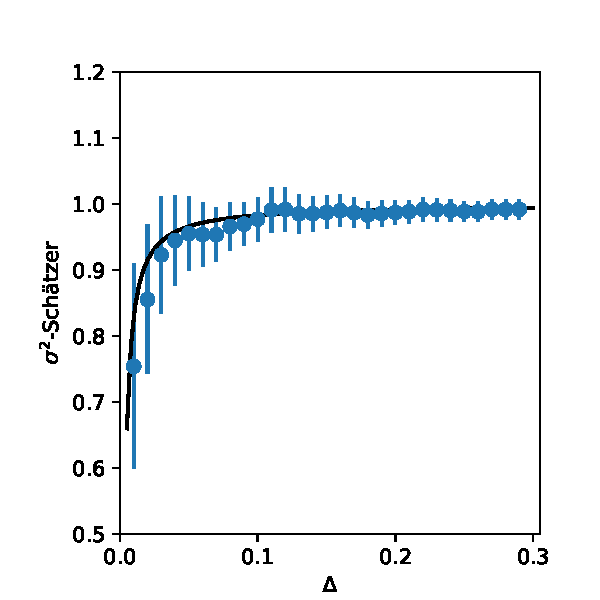
\includegraphics[width=0.5\textwidth]{plots/error}
  \caption{Geschätzte, scheinbare Varianz der Komponenten der
    Geschwindigkeitsverteilung in einem dünnen temperierten
    Lennard-Jones-Systems als Funktion der gewählten Schrittweite
    $\Delta$. Analytisch erwartet man bei der gewählten Temperatur
    eine Varianz von 1. Die blauen Balken geben das
    $1\sigma$-Intervall der beobachteten Varianzen an. Die schwarze
    Linie zeigt die Abschätzung der scheinbaren Varianz gemäß
    \eqref{eq:correrrest} als $(1-2\tau_c/(\Delta N))\sigma^2(x)$, was
    gut zu den gemessenen Daten passt.}
  \label{fig:error}
\end{figure}

Abbildung~\ref{fig:error} zeigt die scheinbare Varianz der Verteilung
der einzelnen Komponenten der Geschwindigkeit als Funktion der
gewählten Messschrittweite im weniger dichten thermalisierten
Lennard-Jones-System. Diese Geschwindigkeiten sind im thermischen
Gleichgewicht normalverteilt um die Null mit einer Varianz
proportional zur Temperatur des Systems. Im Falle der hier benutzten
Simulationen stellt ein Thermostat sicher, dass die Temperatur exakt 1
ist. Wie man in Abbildung~\ref{fig:error} allerdings deutlich sieht,
wird mit korrelierten Messungen die Varianz, und damit die Temperatur,
um bis zu 25\% unterschätzt, sofern zwischen den Messungen deutlich
weniger Zeit als die Korrelationszeit des Systems, $\approx 0,17$,
liegt. Im Beispiel wurden alle $0,01$ Schritte insgesamt 50.000 Daten
erhoben. Der quadratische Fehler der beobachteten mittleren
Geschwindigkeitskomponenten ist also $1\cdot 34/50.000 \approx 7\cdot
10^{-4}$ anstatt $2\cdot 10^{-5}$, wie man ohne Berücksichtigung der
Korrelationen erhalten würde.

Im Falle der Temperatur gibt es eine einfache Abhilfe, da die
Temperatur auch aus der kinetische Energie abgeschätzt werden kann,
allerdings ist das nicht immer der Fall. So wird die Wärmekapazität
eines Systems aus der Varianz der Energiedichte bestimmt, und die
dielektrische Konstante aus der Varianz des Dipolmoments. In diesem
Fall ist es also enorm wichtig, mit ausreichend vielen unkorrelierten
Daten zu arbeiten.

\subsection{Binning-Analyse}
\index{Binning}

Im obigen Beispiel ist die Autokorrelationsfunktion tatsächlich
einfach exponentiell und daher die Autokorrelationszeit einfach zu
bestimmen. Bei den meisten komplexen Systemen ist das nicht der Fall.
Trotzdem lässt sich \eqref{eq:correrrest} anwenden, allerdings geht
dann die \emph{integrierte} Autokorrelationszeit
\begin{equation}
  \tau_\text{int} := \frac{1}{C(A,A)(0)}\int_0^\infty C(A,A)(\tau)\,d\tau
\end{equation}
ein. Eine Möglichkeit, diese abzuschätzen, ist die
Binning-Analyse~\cite{janke02a}. Diese Methode liefert direkt den
Messfehler, kann aber auch benutzt werden, um die $\tau_\text{int}$ zu
bestimmen.

Dazu seien die Daten $x$ in $B$ Blöcke (\enquote{Bins}) der Länge $k$
eingeteilt. Ist $N$ nicht durch $k$ teilbar, muss dazu der Datensatz
etwas gekürzt werden, so dass alle Blöcke voll sind. Anstatt der
einzelnen Daten in den Blöcken, betrachten wir nun nur ihre jeweiligen
Mittelwerte
\begin{equation}
  X_{k,l} = \frac{1}{k}\sum_{j=1}^{k}x_{(l-1)k + j}\quad l=1(1)B.
\end{equation}
Offenbar hängen der Erwartungswert und die Varianz der einzelnen
$X_{k,l}$ nicht vom Aufpunkt $l$ ab. Wir schreiben daher kurz $X_k$
für die Observable der Blockmittelwerte der Länge $k$.  Der
Erwartungswert von $X_k$ ist unverändert der von $x$, also $\mean{X_k}
= \mean{x}$, und auch für den Mittelwert aller $X_k$ gilt $\bar{X} =
\bar{x}$. Allerdings ist die Varianz $\sigma^2(X_{k})$ im allgemeinen
von $\sigma^2(x)$ verschieden, und zwar abhängig von $k$. Sofern $k$
sehr viel größer als die typischen Korrelationslängen ist, gilt nach
\eqref{eq:errestvarcorr} $\sigma^2(X_{k}) \approx
\sigma^2(x)/k_\text{eff}$, wobei $k_\text{eff} = k \Delta /
(2\tau_\text{int})$ die effektive Anzahl der unabhängigen Messungen
ist. Für sehr kleine $k$ hingegen spielt die Mittelung keine Rolle,
daher ist $\sigma^2(X_{k}) \approx \sigma^2(x)$.

Diese Verhalten nutzen wir nun, um den Fehler korrelierter Daten
abzuschätzen. Dazu berechnen wir den quadratischen Fehlerschätzer
\eqref{eq:esterr} für die Blockmittelwerte bei verschiedenen
Blockgrößen $k$:
\begin{equation}
  \epsilon^2(k) := \frac{1}{B - 1} \left(\overline{X_k^2} -
    \overline{X_k}^2\right) \approx \frac{k}{N} \sigma^2(X_k).
\end{equation}
Ist $k$ klein, so ist $\sigma^2(X_k)\approx \sigma^2(x)$, und
$\epsilon^2(k)$ wächst linear in $k$. Für große $k$ hingegen ist
$\sigma^2(X_k) \approx \sigma^2(x)/k_\text{eff}$, so dass
$\epsilon^2(k)$ konstant wird, und zwar
\begin{equation}
  \epsilon^2(k)= \frac{k}{N}\frac{\sigma^2(x)}{k_\text{eff}} =
  \frac{\sigma^2(x)}{N_\text{eff}}.
\end{equation}
Der konstante Wert bei großen $k$ ist also der gesuchte tatsächliche
Fehler!  Allerdings stehen bei großen $k$ für die Mittelung immer
weniger Blöcke zur Verfügung, so dass $\epsilon^2(k)$ stark
verrauscht. Daher funktioniert diese Analyse nur, sofern man genügend
Daten gesammelt hat. Auch die Umkehrung gilt: trägt man
$\epsilon^2(k)$ gegen $k$ auf und sieht kein Plateau bei großen $k$,
hat man noch nicht genügend Daten gesammelt, um eine Aussage über die
Güte der Messung zu machen, man benötigt also mehr Daten.

Neben des Fehlers lässt sich für große $k$ auch die integrierte
Autokorrelationszeit gemäß
\begin{equation}
  \label{eq:tauint}
  k \Delta\frac{\sigma^2(X_k)}{\sigma^2(x)} \approx
  \frac{k\Delta}{k_\text{eff}} = 2\tau_\text{int}
\end{equation}
bestimmen, wobei die Messung von $\sigma^2(x)$ ausreichend unabhängige
Daten voraussetzt. Dies überprüft man zunächst anhand von
$\epsilon^2(k)$.

\begin{figure}
  \centering
  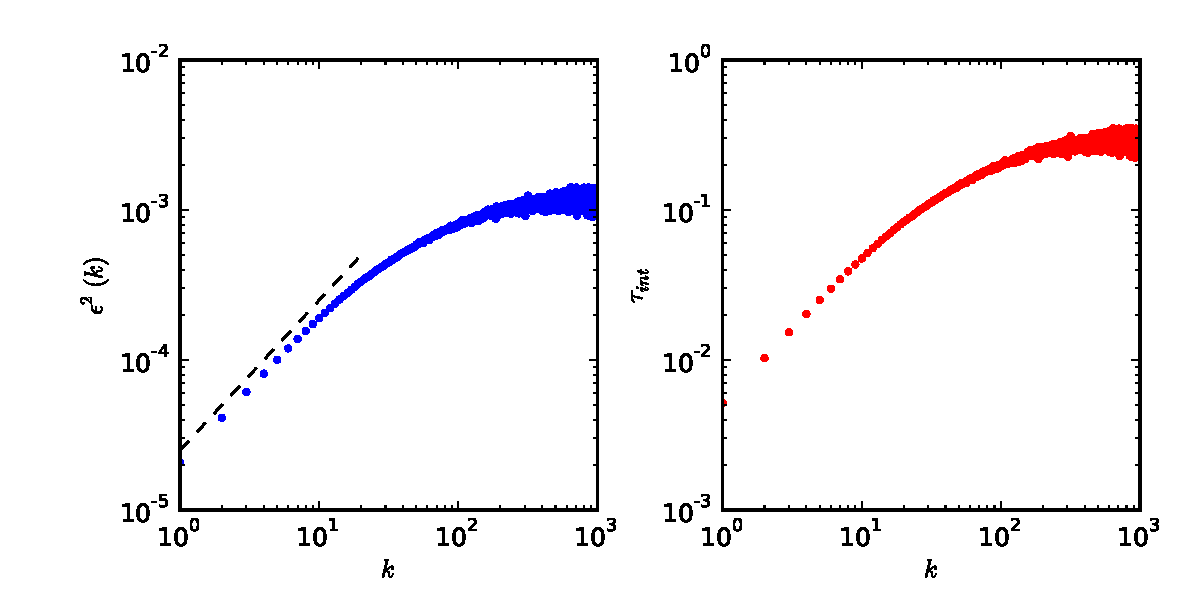
\includegraphics[width=\textwidth]{plots/binning}
  \caption{Links: geschätzter quadratischer Fehler $\epsilon^2(k)$ in
    der Messung der Komponenten der Geschwindigkeitsverteilung in
    einem dünnen temperierten Lennard-Jones-Systems als Funktion der
    Blockgröße $k$. Der Fehler erreicht sein Plateau bei etwa
    0,001, was gut mit der Abschätzung über die Autokorrelationszeit
    übereinstimmt.  Die gestrichelte schwarze Linie demonstriert das
    lineare Wachstum für kleine $k$. Rechts: Geschätzte integrierte
    Autokorrelationszeit $\tau_\text{int}$ für dasselbe System.  Diese
    erreicht ihr Plateau bei $\tau_\text{int} \approx 0,25$, was etwas
    größer als $\tau_c$ ist.}
  \label{fig:binning}
\end{figure}

Abbildung~\ref{fig:binning} demonstriert die Abschätzung des
quadratischen Fehlers und der integrierten Autokorrelationszeit für
die Messung der Geschwindigkeitskomponenten in der
Lennard-Jones-Flüssigkeit. Wie erwartet werden beide Größen für große
$k$ konstant, aber sind verrauscht, während sie für kleine $k$ linear
anwachsen.  Für die Bestimmung der integrierten Autokorrelationszeit
wurde das analytische Ergebnis $\sigma^2(x)=1$ benutzt, die gemessene
ist mit $1,03$ etwas größer. Aus der Binning-Analyse ergibt sich ein
quadratischer Fehler von etwa 0,001 und eine integrierte
Autokorrelationszeit von 0,25, was gut zu unserer Autokorrelationszeit
$0,17$ und der Fehlerschätzung von $7\cdot 10^{-4}$ passt.

\section{Ausgleichsrechnung, Methode der kleinsten Quadrate}
\index{Ausgleichsrechnung}
\index{Fitting}
\index{Methode der kleinsten Quadrate}

\begin{figure}
  \centering
  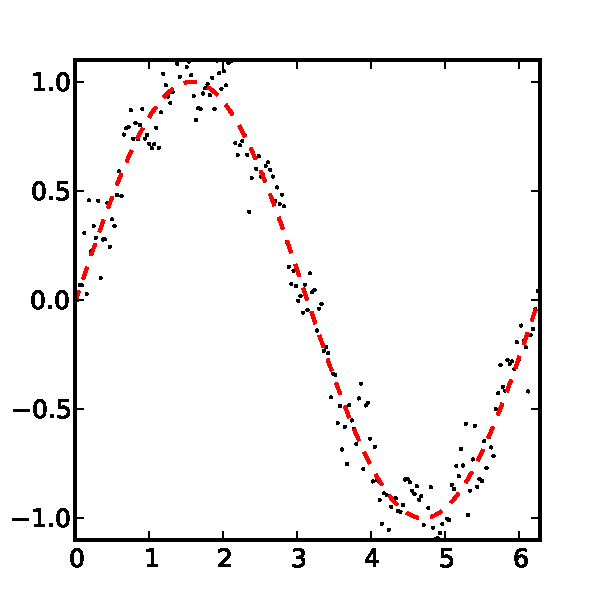
\includegraphics[width=0.5\textwidth]{plots/leastsq}
  \caption{Methode der kleinsten Quadrate zum Fitten der Sinusfunktion
    $y=\sin(x)$. 200 Datenpunkte zwischen 0 und $2\pi$ wurden als
    $\sin(x) + 0,1\,\sin(10 x) + \xi$ erzeugt, wobei $\xi$ eine
    Gauß-verteilte Pseudozufallsvariable mit Varianz $0,01$ war. Die
    resultierende Sinusfunktion (rot gestrichelt) hat die Form $a
    \sin(bx+c)$, wobei die Koeffizienten auf gut 2\% Genauigkeit
    $a=b=1$ und $c=0$ entsprechen. Die kleine höherfrequente
    Schwingung kann durch einen Fit allerdings nicht zuverlässig
    erkannt werden, anders als durch eine Fouriertransformation,
    vergleiche Abbildung~\ref{fig:fourieralias}}
  \label{fig:leastsq}
\end{figure}

Interpolierende Polynome, Taylorreihen und Splines haben gemeinsam,
das diese möglichst nahe an alle gegebenen Stützstellen verlaufen. Die
Anzahl der Terme in der Approximation ist nur durch die Anzahl der
Stützstellen begrenzt, und meist wählt man so viele Stützstellen wie
möglich, um eine möglichst genaue Näherung der unbekannten
Funktionsform zu erhalten.

Wenn die Daten an den Stützstellen aus Experimenten oder
Computersimulationen gewonnen werden, ist das aber gar nicht
gewünscht, da die Daten selbst nicht exakt sind. Wie wir gesehen
haben, kann deren Qualität zwar durch Mittelung verbessert werden,
trotzdem bleibt eine gewisse Unsicherheit.  Andererseits hat man in
diesem Fall üblicherweise eine Vorstellung aus der Theorie, welche
funktionelle Form die Daten annehmen, und möchte nun wissen, bei
welcher Parameterwahl diese Funktion am besten mit den Daten
verträglich ist. Man möchte also den Parametersatz bestimmen, der den
Abstand der Daten von der Funktion minimiert. Dabei ist bei sinnvollen
Experimenten die Anzahl der Datenpunkte sehr viel größer als die
Anzahl der Parameter.

Seien also wieder Daten $(x_i, y_i)$, $i=0(1)n-1$ und eine Funktion
$f_v(x)$ gegeben. Gesucht ist dann derjenige Parametervektor $v$, der
die Abweichung
\begin{equation}
  \label{eq:leastsq}
  \Delta(v) = \sum_i (f_v(x_i) - y_i)^2
\end{equation}
minimiert. Dieses Verfahren wird auch Methode der kleinste Quadrate
genannt, da ja die quadrierten Abweichungen minimiert werden
sollen. Ist $f_{a,b}(x) = ax + b$ eine Gerade, spricht man auch von
\emph{linearer Regression}\index{lineare Regression}. In diesem Fall lässt
sich das Optimum einfach bestimmen, da
\begin{equation}
  0 = \frac{d}{da} \Delta(a,b) = \sum_i 2 (a x_i + b - y_i)x_i
  = 2n \left(a  \overline{x_i^2} + b \overline{x_i} -
    \overline{y_ix_i} \right)
\end{equation}
und
\begin{equation}
  0 = \frac{d}{db} \Delta(a,b) = \sum_i 2 (a x_i + b - y_i)
  = 2n \left(a  \overline{x_i} + b - \overline{y_i} \right),
\end{equation}
wobei $\overline{x} = \frac{1}{n} \sum_{i=0}^{n-1} x_i$ den Mittelwert
über alle Datenpunkte bedeutet. Daraus ergibt sich
\begin{equation}
  a = \frac{\overline{y_ix_i} -
    \overline{y_i}\cdot\overline{x_i}}{\overline{x_i^2}-\overline{x_i}^2}
  \quad\text{und}\;
  b = \overline{y_i} - a \overline{x_i},
\end{equation}
was sich einfach auf dem Computer berechnen lässt.

Auch für quadratische und andere einfache Funktionen lassen sich die
Koeffizienten geschlossen darstellen, aber bei allgemeinen Funktionen
ist dies nicht immer der Fall. Dann muss die nichtlineare
Optimierungsaufgabe \eqref{eq:leastsq} numerisch gelöst werden, was
wir später behandeln werden. Für den Moment genügt uns, dass SciPy die
Funktion \scipy{scipy.optimize.leastsq(delta, v0, (x, y))} dafür
bereitstellt. \argd{(x, y)} sind dabei die Ausgangsdaten, die hier zu
einem Tupel zusammengefasst sind. \argd{v0} ist der Startwert für die
Berechnung, der nicht zu weit vom (unbekannten) Optimum entfernt
liegen darf. \argd{delta} ist eine Python-Funktion, die als Argumente
$v$, $x_i$ und $y_i$ nimmt und $f_v(x_i) - y_i$ zurückliefert.  Da
$f_v(x)$ eine beliebig komplizierte Form annehmen kann, ist diese
Aufgaben im Allgemeinen nicht lösbar, allerdings funktioniert ein
solcher \emph{Fit} für einfache Funktionen meistens recht
gut. Abbildung~\ref{fig:leastsq} zeigt einen solchen Funktionsfit an
eine verrauschte Sinusfunktion, die mit 200 Datenpunkten auf etwa 2\%
genau gefittet werden kann. Man beachte, das der Ausgangswert für den
Fit mit Hilfe der SciPy-Funktion \lstinline!leastsq! $a=0$, $b=1$,
$c=0$ war; beim Startwert $a=0$, $b=0$, $c=0$ bricht das Verfahren
ab. Das zeigt, dass man tatsächlich nicht zu weit vom Optimum starten
kann, was ein gewisses Verständnis der Zielfunktion voraussetzt.

Ist die Funktionsform, die den Daten zugrundeliegt, unbekannt, ist es
normalerweise keine gute Idee, die Form zu raten. Generell sollte auch
die Anzahl der Parameter sehr klein sein, da sich sonst fast alles
"`gut"' fitten lässt ("`With four parameters I can fit an elephant and
with five I can make him wiggle his trunk."' --- J. von Neumann).

Soll aber zum Beispiel für Visualisierungszwecke eine ansprechende
Kurve entlang der Daten gelegt werden, deren tatsächliche Abhängigkeit
unbekannt ist, dann sind \emph{Pad\'e-Funktionen} oft eine gute
Wahl. Diese haben die Gestalt $P(x)/Q(x)$, wobei $P$ und $Q$ zwei
Polynome mit paarweise verschiedenen Nullstellen sind. Üblicherweise
lassen sich schon für niedrige Polynomgrade ansprechende Fits finden,
sofern die Grade der beiden Polynome in etwa gleich gewählt werden.

%%% Local Variables: 
%%% mode: latex
%%% TeX-master: "padc"
%%% TeX-PDF-mode: t
%%% End: 

% Dies ist Teil der Vorlesung Physik auf dem Computer, SS 2012,
% Axel Arnold, Universitaet Stuttgart.
% 
% Dieses Werk ist unter einer Creative Commons-Lizenz vom Typ
% Namensnennung-Weitergabe unter gleichen Bedingungen 3.0 Deutschland
% zugänglich. Um eine Kopie dieser Lizenz einzusehen, konsultieren Sie
% http://creativecommons.org/licenses/by-sa/3.0/de/ oder wenden Sie sich
% schriftlich an Creative Commons, 444 Castro Street, Suite 900, Mountain
% View, California, 94041, USA.

\chapter{Nichtlineare Gleichungssysteme}
\index{Nullstellensuche}
\index{Fixpunktsuche}

Im zweiten Kapitel hatten wir uns mit der Lösung linearer
Gleichungssysteme beschäftigt, die ja eine wesentliche Grundlage der
numerischen Mathematik darstellen. Allerdings tauchen in der Praxis,
besonders in der Physik, leicht auch nichtlineare Gleichungssysteme
auf. In diesem Fall kann man meist keine allgemeine Aussage über
Existenz und Anzahl der Lösungen machen und auch keine exakten
Verfahren zur Lösung angeben.

Nichtlineare Gleichungssysteme werden typischerweise in zwei Formen
betrachtet. Sei eine Funktion $f:M\subseteq\RR^n\to\RR^n$ gegeben. Dann suchen
wir die \emph{Nullstellen}
\begin{equation}
  \label{eq:nullstellen}
  x, \quad\text{so dass}\; f(x) = 0,
\end{equation}
also die Lösungen zur Gleichung $f(x) = 0$. Man beachte, dass anders
als im Fall der linearen Gleichungssysteme gefordert wird, dass der
Bildraum wie auch der Ursprungsraum $M$ zu einem Vektorraum derselben
Dimension $n$ gehören. Ohne diese Voraussetzung ist eine eindeutige
Lösung im Allgemeinen unmöglich. Anders als im Falle der linearen
Gleichungssysteme ist es hier auch nicht ohne Weiteres möglich, den
Lösungsraum anzugeben, falls die Lösung nicht eindeutig
ist. Tatsächlich kann der Lösungsraum ja eine beliebig komplexe
Mannigfaltigkeit innerhalb $M$ darstellen, die dann gar nicht
geschlossen parametrisiert werden kann. Das macht die numerische
Bestimmung dieser Lösungsmannigfaltigkeit sehr schwierig.

Alternativ können wir für eine Funktion $g:M\subseteq\RR^n\to\RR^n$ die
\emph{Fixpunkte} suchen. Diese sind
\begin{equation}
  \label{eq:fixpunkt}
  x, \quad\text{so dass}\; g(x) = x,
\end{equation}
also die Lösungen der Gleichung $g(x) = x$. Eine Fixpunktgleichung
lässt sich natürlich stets auch als Nullstellenproblem mit $f(x) =
g(x) - x$ formulieren und umgekehrt.

Die beiden Formulierungen unterscheiden sich allerdings im natürlichen
Lösungsansatz. Die Nullstellengleichung \eqref{eq:nullstellen} ähnelt
dem linearen Gleichungssystem \eqref{eq:lgs}. Das
\emph{Newtonverfahren} beruht auf einer lokalen Linearisierung und dem
Lösen dieses linearen Gleichungssystems. Die Fixpunktgleichung
hingegen legt nahe, den Fixpunkt durch \emph{sukzessive Substitution}
zu suchen: $x_0\to g(x_0)\to g(g(x_0))\to\ldots$.

\section{Sukzessive Substitution}
\index{sukzessive Substitution}
\index{Fixpunktsuche}

Eine Abbildung $g:M\to M$ mit $M\subset\RR^n$ heißt Lipschitz-stetig
(L-stetig), falls es ein $L\in\RR$ gibt, so dass
\begin{equation}
  \norm{g(x) - g(y)} \le L \norm{x - y}\quad\forall x,y\in M.
\end{equation}
Alle auf $M$ differenzierbaren Funktionen mit beschränkter Ableitung
sind L-stetig, wenn ihre Ableitung beschränkt ist. Die
Lipschitzkonstante ergibt sich aus dem Mittelwertsatz zu $L=\max_{x\in
  M}\norm{g'(x)}$.  Es gibt allerdings noch mehr L-stetige Funktionen,
zum Beispiel die in 0 nicht differenzierbare Betragsfunktion, die auf
ganz $\RR$ L-stetig mit $L = 1$ ist. Auf der anderen Seite ist
offenbar jede L-stetige Funktion auch stetig, \dh\,, die L-stetigen
Funktionen sind eine eigene Klasse zwischen den stetigen und
differenzierbaren Funktionen. Dabei ist es nicht wesentlich, welche
Norm $\norm{\cdot}$ genutzt wird. Sie kann für das Problem geeignet
gewählt werden, sofern sie die üblichen Bedingungen an eine Norm, wie
etwa die Dreiecksungleichung, erfüllt.

\index{Banachscher Fixpunktsatz} Hat eine Funktion $g:M\to M$ eine
Lipschitz-Konstante $L<1$, so heißt $g$ \emph{kontrahierend}, weil
zwei verschiedene Punkte durch die Abbildung stets näher aneinander
geschoben werden. Wir betrachten nun einen beliebigen Startpunkt
$x_0\in M$ und definieren damit die Folge der \emph{sukzessiven Substitution}:
\begin{equation}
  x_{n} := g(x_{n-1}) \quad\text{für}\; n\ge 1.
\end{equation}
Dann gilt für alle $n,m\in\NN$ der \emph{Banachsche Fixpunktsatz}
\begin{align}
  \label{eq:banach}
  \norm{x_{n+m} - x_n} \,=\, &\norm{\sum_{k=0}^{m-1} x_{n+k+1} - x_{n+k}}
  \,\le\, \sum_{k=0}^{m-1} \norm{x_{n+k+1} - x_{n+k}}\nonumber\\
  \,=\, &\norm{g(g(\ldots g(x_{n+1}))) - g(g(\ldots g(x_{n})))}
  + \cdots\nonumber\\
  &+ \norm{g(g(x_{n+1})) - g(g(x_{n}))}
  + \norm{g(x_{n+1}) - g(x_{n})} + \norm{x_{n+1} - x_{n}}\nonumber\\
  \le\, &\sum_{k=0}^{m-1} L^k \norm{x_{n+1} - x_{n}}
  \,\le\, \frac{1}{1-L}\norm{x_{n+1} - x_{n}} \le
  \frac{L^n}{1-L}\norm{g(x_0) - x_0}.
\end{align}
Die sukzessive Substitution definiert also eine Cauchyfolge, die in
$M$ konvergiert, sofern $M$ abgeschlossen ist (\zb $M=\RR^n$ oder $M$
Einheitskugel). Für den Grenzwert $\overline{x}$ dieser Folge gilt
\begin{equation}
  \overline{x} = \lim_{n\to\infty}x_{n+1} = \lim_{n\to\infty}g(x_{n})
  = g(\overline{x}),
\end{equation}
er ist also ein Fixpunkt.

Wir betrachten nun zwei Fixpunkte $\overline{x}$ und $\overline{y}$. Dann gilt
\begin{equation}
  \norm{\overline{x} - \overline{y}} = \norm{g(\overline{x}) -
    g(\overline{y})} \le L \norm{\overline{x} - \overline{y}} \implies
  \overline{x} = \overline{y}.
\end{equation}
Das bedeutet, dass es nur genau einen Fixpunkt $\overline{x}$ von $g$
in $M$ gibt, und dass die sukzessive Substitution für jeden Startwert
\emph{global} gegen $\overline{x}$ konvergiert. \eqref{eq:banach}
gibt auche eine \textit{a priori}-Abschätzung des Fehlers:
\begin{equation}
  \norm{\overline{x} - x_n} \le \frac{L^n}{1-L}\norm{g(x_0) - x_0}
\end{equation}
sowie eine Abschätzung der Konvergenzrate:
\begin{equation}
  \frac{\norm{x_{n+1} - \overline{x}}}{\norm{x_n - \overline{x}}}
  = \frac{\norm{g(x_n) - g(\overline{x})}}{\norm{x_n - \overline{x}}}
  \le L < 1.
\end{equation}
Die sukzessive Substitution konvergiert also linear. Das Verfahren
wird abgebrochen, wenn $\norm{x_{n+1} - x_n}$ hinreichend klein ist,
da dann nach \eqref{eq:banach} auch
\begin{equation}
  \norm{\overline{x} - x_n} \le \frac{1}{1-L}\norm{x_{n+1} - x_n}.
\end{equation}
Offenbar konvergiert die sukzessive Substitution um so schneller, je
kleiner die Lipschitzkonstante $L$ ist.

Neben der globalen Konvergenzeigenschaft konvergiert die sukzessive
Substituion auch lokal: ist $g:\RR^n\to\RR^n$ eine differenzierbare
Funktion und hat einen Fixpunkt $\overline{x}$ mit $\norm{g'(x)} < 1$,
so gibt es eine Umgebung des Fixpunktes, in dem die sukzessive
Substitution gegen diesen Fixpunkt konvergiert.

\begin{figure}
  \centering
  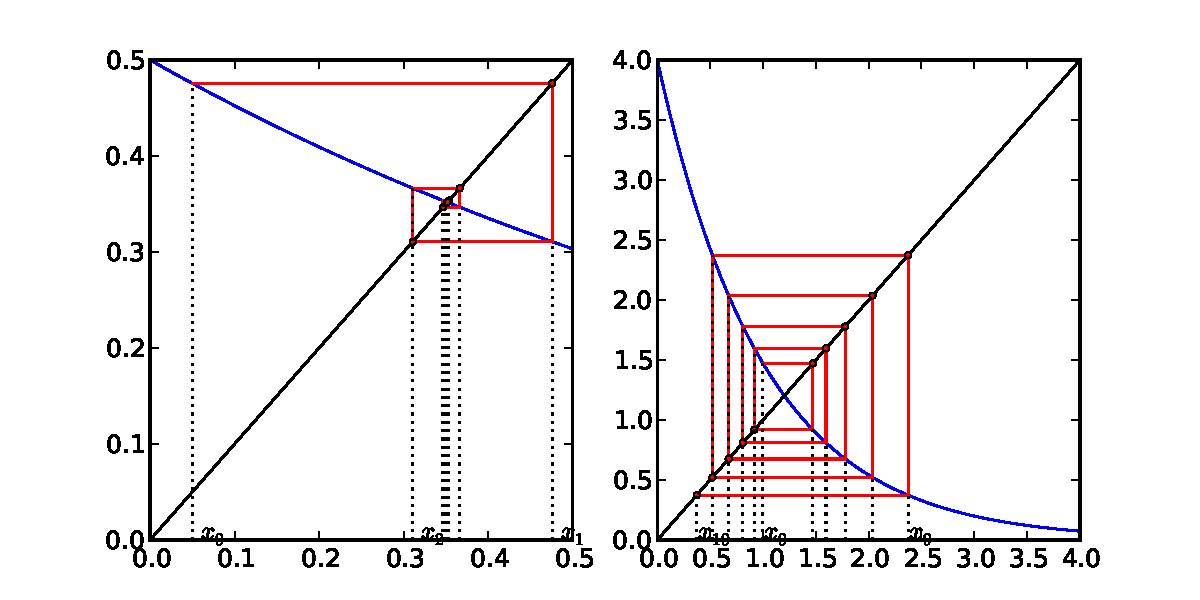
\includegraphics[width=\textwidth]{plots/banach}
  \caption{Sukzessive Substitution mit Funktion $g(r) = e^{-r}/\phi_0$
    mit $\phi_0=2$ (links) und $\phi_0=1/4$ (rechts). Blau
    durchgezogen ist die Funktion $g$, die Winkelhalbierende ist
    schwarz dargestellt. Die Punkte auf der Winkelhalbierenden
    markieren die Punkte $(x_1,x_1)$, $(x_2,x_2)$ \usw\,, durch die das
    Lot auf $g$ gefällt wird, um den nächsten Punkt der sukzessiven
    Substitution zu erhalten. Im linken Graph sind die ersten sieben
    Glieder dargestellt, die exponentielle Konvergenz ist gut zu
    sehen. Im rechten Graph konvergiert das Verfahren nicht mehr.}
  \label{fig:banach}
\end{figure}

\subsection{Beispiel}

Als Beispiel für eine Anwendung des Banachschen Fixpunktsatzes
betrachten wir die dimensionslose Form des Yukawa- oder
Debye-Hückel-Potentials $\phi(r) = e^{-r}/r$. Wir fragen uns, wann für
welches $r$ dieses Potential einen gegeben Wert $\phi_0$ annimmt. Das
führt zu der Fixpunktgleichung
\begin{equation}
  g(r) = \frac{e^{-r}}{\phi_0} = r
\end{equation}
Die linke Seite ist eine auf $[0,\infty)$ L-stetige Funktion mit
$L=1/\phi_0$, wie man durch Ableiten leicht sieht.

Abbildung~\ref{fig:banach} zeigt die sukzessive Substitution für
$g(r)$. Graphisch lässt sich das Verfahren visualisieren, indem in
jeder Iteration der Funktionswert $x_{n+1} = y =g(x_{n})$ an der
Winkelhalbierenden $y=x$ auf die $x$-Achse zurückgespiegelt wird. Im
linken Graph ist $\phi_0=2$ und damit $L=1/2$, so dass die sukzessive
Substitution exponentiell konvergiert. Für das letzte abgebildete
Glied, $x_7$, gilt $\abs{x_7-\overline{x}} \le 1/2^8 = 1/256$. Im
rechten Graph ist $\phi_0=1/4$ und damit $L=4$. Insbesondere ist auch
im Fixpunkt $g'(\overline(x))>1$. Abgebildet sind die ersten zehn
Glieder der sukzessiven Substitution, die hier nicht mehr
konvergiert. Wird hingegen $\phi_0$ so gewählt, dass 
$g'(\overline(x))<1$, aber $L>1$, so konvergiert das Verfahren zwar
noch, aber nicht mehr exponentiell.

\section{Newtonverfahren in einer Dimension}
\index{Newtonverfahren}
\index{Nullstellensuche}

Nachdem wir bis jetzt die sukzessive Substitution zur Bestimmung von
Fixpunkten betrachtet haben, geht es nun um die Nullstellensuche. Sei
also zunächst eine stetig differenzierbare Funktion $f:[a,b]\to\RR$
gegeben und deren Nullstellen $x$, $f(x) = 0$, gesucht. Ähnlich wie
bei der sukzessiven Iteration starten wir mit einem Startwert
$x_0$. Um uns nun der Nullstelle der Funktion zu nähern, linearisieren
wir in der aktuellen Näherung $x_n$ und lösen nach der Nullstelle
$x_{n+1}$ auf:
\begin{equation}
  x_{n+1} = g(x_n) := x_n - \frac{f(x_n)}{f'(x_n)}\quad\text{für}\; n\ge 0,
\end{equation}
wobei wir annehmen, dass $f'(x)\neq 0$ auf $[a,b]$.  Für eine
Nullstelle $\overline{x}$ von $f$ gilt offenbar $g(\overline{x}) =
\overline{x}$, \dh wir suchen einen Fixpunkt von $g$, den wir wieder
durch sukzessive Substitution annähern können. Man bricht das
Verfahren wie auch die sukzessive Substitution ab, wenn
$\abs{x_{n}-x_{n-1}}$ bzw. $\abs{f(x_n)}$ hinreichend klein sind.

\begin{figure}
  \centering
  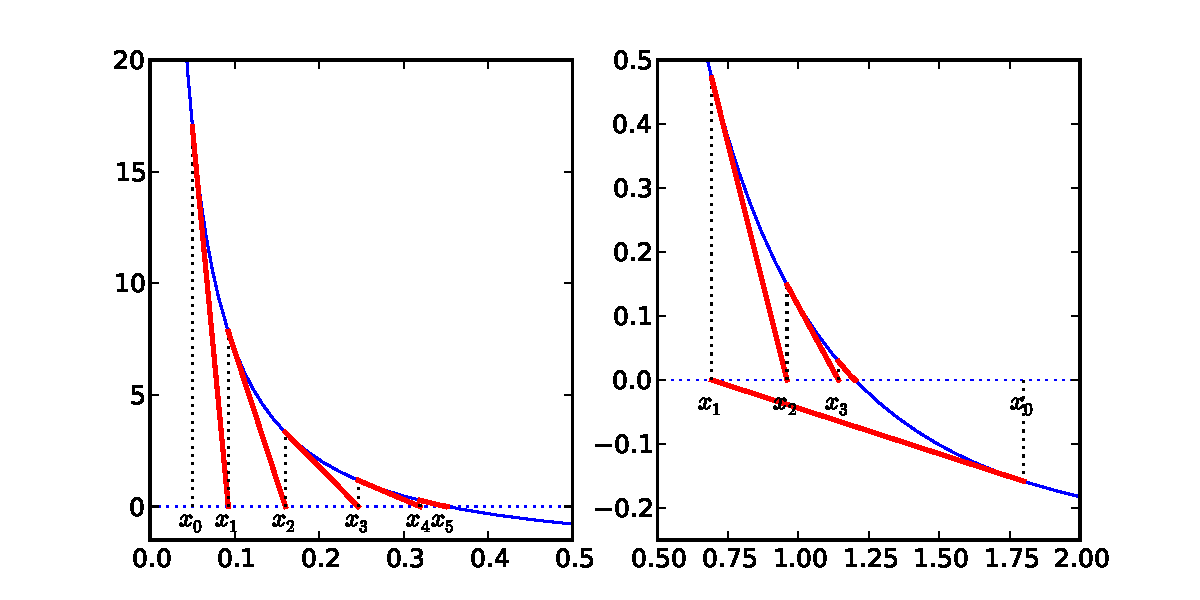
\includegraphics[width=\textwidth]{plots/newton}
  \caption{Newtonverfahren für die Funktion $f(r) = e^{-r}/r -
    \phi_0$. Wie schon beim Graphen zur sukzessiven Substitution ist
    links $\phi_0=2$, rechts $\phi_0=1/4$, allerdings konvergiert das
    Newtonverfahren für beide Werte. Blau dargestellt ist $f$, die
    roten, dicken Linien stellen die Tangenten dar, deren Nullstellen
    die neuen Näherungen für die gesuchte Nullstelle von $f$ sind.}
  \label{fig:newton}
\end{figure}

Ist nun $f$ sogar zweifach stetig differenzierbar, so gilt
\begin{equation}
  g'(x) = 1 - \frac{f'(x)^2 - f(x)f''(x)}{f'(x)^2} =
  \frac{f(x)f''(x)}{f'(x)^2} \implies g'(\overline{x}) = 0.
\end{equation}
Das Newtonverfahren konvergiert also zumindest lokal gegen einen
Fixpunkt $\overline{x}$ von $g$ beziehungsweise eine Nullstelle von
$f$. Tatsächlich konvergiert das Verfahren wenigstens quadratisch,
wenn $f$ zweifach differenzierbar ist, da
\begin{align}
  x_{n+1} - \overline{x} = \frac{(x_n - \overline{x})f'(x_n) -
    f(x_n)}{f'(x_n)}
  = \frac{(x_n - \overline{x})}{f'(x_n)}\left( f'(x_n) -
    \frac{f(x_n) - f(\overline{x})}{x_n - \overline{x}}\right)\nonumber\\
  = \frac{(x_n - \overline{x})}{f'(x_n)}\left( f'(x_n) -
    f'(\xi')\right)
  = \frac{(x_n - \overline{x})(x_n - \xi')}{f'(x_n)}f''(\xi)
\end{align}
und somit
\begin{equation}
  \frac{\abs{x_{n+1} - \overline{x}}}{\abs{x_n - \overline{x}}^2}
  \le \frac{\max_{\xi\in [a,b]} \abs{f''(\xi)}}{\min_{\xi\in [a,b]} \abs{f'(\xi)}}
\end{equation}
Ist $f$ nur differenzierbar, so lässt sich ähnlich zeigen, dass das
Newtonverfahren superlinear konvergiert. Das Newtonverfahren
konvergiert also in jedem Fall schneller als die sukzessive
Substitution, erfordert allerdings eine mindestens stetig
differenzierbare Funktion.

Bis jetzt haben wir nur die lokale Konvergenz des
Newton-Verfahrens. Ist die Zielfunktion $f\in C^1([a,b])$ allerdings
konvex bzw.\ konkav, also $f'$ monoton wachsend bzw.\ fallend und
beschränkt, und hat $f$ eine Nullstelle in $[a,b]$, so kann man
zeigen, dass das Newtonverfahren global gegen eine Nullstelle
$\overline{x}$ von $f$ in $[a,b]$ konvergiert. Dabei ist das Verfahren
nach dem ersten Schritt monoton, \dh entweder $x_1\le
x_2\le\ldots\le\overline{x}$ oder $x_1\ge
x_2\ge\ldots\ge\overline{x}$.

In SciPy gibt es natürlich auch das Newtonverfahren sowie einige
verbesserte Algorithmen. Das Newtonverfahren ist als
\scipy{scipy.optimize.newton(f, x0, df)} implementiert, wobei \argd{f}
und \argd{df} die Funktion $f$ und ihre Ableitung $\nicefrac{df}{dx}$
angeben, und \argd{x0} der Startwert des Newtonverfahrens.

\subsection{Beispiel}

Wir betrachten wieder die Aufgabe $e^{-r}/r = \phi_0$, bzw. $f(r) =
e^{-r}/r - \phi_0 = 0$. Die Ableitung dieser Funktion ist $-e^{-r}(1 +
r)/r^2$, $f$ fällt also monoton. Daher konvergiert das Newtonverfahren
global und monoton, wie in Abbildung~\ref{fig:newton} zu sehen. Im
linken Graphen ist $r_0<\overline{r}$, daher startet das Verfahren
sofort monoton. Im rechten Graphen ist $r_0 < \overline{r}$. Hier wird
im ersten Schritt $r_1 < \overline{r}$, und erst dann wächst die
Näherung wieder monoton. In jedem Fall konvergiert das
Newtonverfahren, anders als die sukzessive Substitution, für beide
Werte von $\phi_0$ innerhalb weniger Schritte zuverlässig gegen die
Nullstelle.

\subsection{Wurzelziehen}

Wir betrachten die Gleichung $f(x) = x^k - a = 0$ auf der positiven
Halbachse. Dann konvergiert für jeden Startwert $x_0>0$ das
Newtonverfahren
\begin{equation}
  x_{n+1} = x_n - \frac{f(x_n)}{f'(x_n)} = \left(1 -
    \frac{1}{k}\right) x_n + \frac{1}{k} \frac{a}{x_n^{k-1}}
\end{equation}
gegen die einzige Nullstelle, nämlich die $k$-te Wurzel aus
$a$. Sinnvollerweise wählt man daher $x_0=a$ als Startwert. Für $k=2$
ergibt sich das \emph{Heron-Verfahren} $x_{n+1} = \frac{1}{2}\left(x_n
  + \frac{a}{x_n}\right)$, das bereits im 2.\ Jhdt.\ vor Christus zum
Wurzelziehen benutzt wurde.

Für die Wurzel aus $a=2$ sind die ersten 5 Schritte des Heronverfahrens:
\begin{center}
  \begin{tabular}{r|l|l}
    Schritt $n$ & $x_n$ & Anzahl korrekter Stellen \\\hline
    0 & 1.000000000000000 & 1 \\
    1 & 1.500000000000000 & 1 \\
    2 & 1.416666666666667 & 2 \\
    3 & 1.414215686274510 & 5 \\
    4 & 1.414213562374690 & 11 \\ 
    5 & 1.414213562373095 & 15
  \end{tabular}
\end{center}
Mit der auf Rechnern üblichen doppelten Genauigkeit ist das Verfahren
damit auskonvergiert.

Die Anzahl der Rechenoperationen für $n$ Schritte entspricht der
Auswertung eines Polynoms mit $3n/2$ Koeffizienten. Wäre man zum
Beispiel nur an der Wurzel im Bereich $[0,5]$ interessiert und würde
hierzu ein interpolierendes Polynom mit 7 Chebyshev-Stützstellen
nutzen, wäre $\sqrt{2}\approx 1.40966$ mit gerade einmal einer
korrekten Stelle. Mit einer Taylorentwicklung um 1 würde es etwas
besser. Bei 7 Termen liefert diese $\sqrt{2}\approx 1.4214$ mit 2
korrekten Stellen.

Für $k=-1$ wird aus der Wurzelaufgabe eine Division, da wir die
Nullstelle der Funktion $f(x) = \frac{1}{x} - a$ suchen. Die Lösung
kann nur mit Hilfe der Grundrechenarten durch die Iteration
\begin{equation}
  x_{n+1} = x_n - \frac{f(x_n)}{f'(x_n)} = 2x_n - a x_n^2 
\end{equation}
bestimmt werden. Allerdings ist die Ableitung von $a/x$ unbeschränkt,
daher konvergiert das Verfahren nur für Startwerte, die hinreichend
nah an der Lösung sind. Wie man sich in diesem Fall leicht überlegt,
konvergiert das Verfahren nur für $x_o\in (0, 2/a)$, was schwierig zu
erfüllen ist, ohne $a^{-1}$ bereits zu kennen.

\subsection{Nullstellen von Polynomen}

Ist $p$ ein Polynom, so lassen sich dessen Nullstellen (approximativ)
mit Hilfe des Newtonverfahrens bestimmen:
\begin{equation}
  x_{n+1} = x_n - \frac{p(x_n)}{p'(x_n)},
\end{equation}
wobei $p(x_n)$ und $p'(x_n)$ durch ein modifiziertes Hornerschema
bestimmt werden können. Die folgende Routine berechnet effizient
$x_{n+1}$ aus $x_n$:%
\lstinputlisting[firstline=10]{horner_newton.py}%
Das Newtonverfahren liefert natürlich nur eine Nullstelle des
Polynoms. Durch die Polynomdivision, wieder mit Hilfe des
Hornerschemas wie in Abschnitt~\ref{sec:horner}, lässt sich diese
aber abspalten und das Newtonverfahren erneut starten, bis alle
Nullstellen gefunden sind.

\section{\keyword{Sekantenmethode}}

\begin{figure}
  \centering
  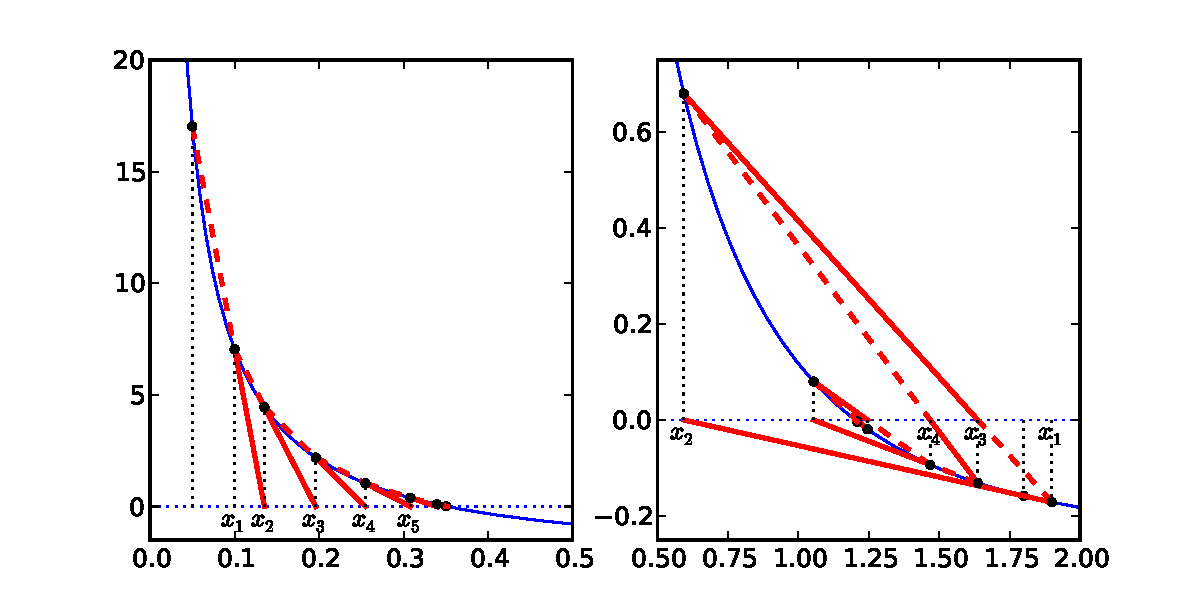
\includegraphics[width=\textwidth]{plots/sekanten}
  \caption{Sekantenmethode für die Funktion $f(r) = e^{-r}/r -
    \phi_0$. Wie zuvor ist links $\phi_0=2$, rechts $\phi_0=1/4$.
    Blau dargestellt ist wieder $f$, die roten, gestrichelten dicken
    Linien stellen die Sekanten dar, deren Nullstellen die neuen
    Näherungen für die gesuchte Nullstelle von $f$ sind. Durchgezogen
    ist der Abschnitt der Sekante durch $x_{n-1}$ und $x_n$, der von $x_n$
    zu $x_{n+1}$ führt.}
  \label{fig:sekanten}
\end{figure}

In vielen Fällen ist es nicht einfach oder unmöglich, die Ableitung
einer Funktion zu bestimmen. In diesem Fall kann man die Ableitung
durch die dividierte Differenz annähern, wobei nun zwei Startpunkte
$x_0$ und $x_1$ gebraucht werden. Dies führt dazu, dass die
Näherungsfunktion keine Tangente mehr ist, wie beim Newtonverfahren,
sondern im Allgemeinen eine Sekante. Daher rührt der Name der
\emph{Sekantenmethode}
\begin{equation}
  x_{n+1} = x_n - f(x_n)\frac{x_n - x_{n-1}}{f(x_n) - f(x_{n-1})},
\end{equation}
die nicht mehr quadratisch, aber wenigstens superlinear konvergiert.

Das Bestimmen der Ableitung von $f$ ist immer dann unmöglich, wenn $f$
sehr komplex ist. Ein Extremfall wäre eine
Molekulardynamik-Computersimulation, bei der zum Beispiel in
Abhängigkeit vom aktuellen Volumen $V$ der mittlere Druck $P(V)$ in
einem gegebenen System bestimmt wird. Den mittleren Druch nach $V$
abzuleiten, ist vollkommen aussichtslos, wenn die Wechselwirkungen
zwischen den Teilchen hinreichend komplex sind. Dabei ist es von
großem Interesse, dasjenige Volumen zu bestimmen, für das $P(V)$
gleich einem vorgegebenen Außendruck $P_0$ ist, denn dies ist die
natürliche Bedingung im isobarischen Ensemble. Dies führt aber zur
Nullstellengleichung $P(V)-P_0 = 0$.

Als Beispiel für die Sekantenmethode soll ein weiteres Mal die
Funktion $f(r) = e^{-r}/r - \phi_0$ dienen. Für diese zeigt
Abbildung~\ref{fig:sekanten} die erste paar Schritte der
Sekantenmethode. Unter geeigneten Umständen, nämlich, wenn die
angenäherte Tangente hinreichend gut mit der tatsächlichen über
einstimmt, konvergiert die Sekantenmethode praktisch genauso gut wie
das normale Newtonverfahren. Sind die Startpunkte allerdings ungünstig
gewählt, wie im rechten Beispiel, so kann es passieren, dass diese
abwechselnd um die Nullstelle liegen, und damit nicht mehr monoton
konvergieren.

In SciPy implementiert \scipy{scipy.optimize.newton(f, x0)} (also bei
Nichtangabe der Ableitung) die Sekantenmethode. \argd{f} ist wieder
die Funktion, deren Nullstelle gesucht wird, und \argd{x0} ein
Startwert. Der zweite wird hardcodiert in einer Umgebung von \argd{x0}
gewählt, kann also vom Benutzer nicht gesetzt werden.

\section{\keyword{Bisektion}}
\index{Bisektionsverfahren}

Wie wir gesehen haben, konvergiert das Newtonverfahren und seine
Varianten sehr schnell, allerdings oft nur unter der Voraussetzung,
dass der Startwert hinreichend nah an einer Nullstelle liegt. Wie aber
kann man einen solchen Startwert finden? Hierfür wird ein langsameres,
robusteres Verfahren gebraucht, zum Beispiel das
\emph{Bisektionsverfahren} in einer Dimension.

Sei also wieder $f\in C([a,b])$ eine stetige Funktion, und
$f(a)f(b)<0$. Dann hat $f$ gemäß Mittelwertsatz wenigstens eine
Nullstelle im Interval $[a,b]$, die wir suchen. Dazu setzen wir
zunächst $a_0=a$ und $b_0=b$. Dann betrachten wir den
Intervallmittelpunkt
\begin{equation}
  m_{n} = \frac{a_n + b_n}{2}.
\end{equation}
Ist $f(m_n)f(a_n) < 0$, hat die Funktion also bei $m_n$ und $a_n$ unterschiedliche Vorzeichen, so
muss eine Nullstelle im halb so großen Interval $a_1=a_0$, $b_1=m_0$
liegen, mit dem wir nun weiter verfahren. Anderfalls ist
notwendigerweise $f(m_n)f(b_n)\le 0$, und die Nullstelle ist im neuen
Interval $a_1=m_0$, $b_1 = b_0$. Ist $b_n - a_n$ kleiner als die
gewünschte Genauigkeit für die Nullstelle, bricht man einfach
ab. $m_n$ ist dann die endgültige Näherung für die Nullstelle.

Das Verfahren halbiert in jedem Schritt die Intervallgröße und damit
auch den maximalen Abstand der Näherung zur tatsächlichen
Nullstelle $\overline{x}$. Es gilt also
\begin{equation}
  \frac{\abs{m_{n+1} - \overline{x}}}{\abs{m_{n} - \overline{x}}}\le \frac{1}{2},
\end{equation}
das Verfahren konvergiert also nur linear, dafür aber global.

In der Praxis kombiniert man die Bisektion mit dem Newtonverfahren, indem
zunächst einige Schritte des Bisektionsverfahrens durchgeführt
werden, und dann vom Intervallmittelpunkt aus das
Newtonverfahren. Konvergiert dieses, so ist man fertig. Läuft das
Newtonverfahren aus dem Bisektionsinterval heraus,
verkleinert man dieses durch weitere Bisektionsschritte, und versucht dann
erneut, das Newtonverfahren anzuwenden.

In Abbildung~\ref{fig:bisektion} dient uns ein letztes Mal die
Funktion $f(x) = e^{-r}/r - 2$ als Beispiel für die Bisektion. Mit
sieben Schritten schließt diese bei Startinterval $[0,1,\,1]$ die
Nullstelle bis auf $[0,3391,\,0,3461]$, als etwa $10^{-2}$ genau
ein. Zum Vergleich: das Newtonverfahren mit Startwert $0,05$ erreicht
in sieben Schritten eine Genauigkeit von etwa $10^{-5}$, und selbst
die Sekantenmethode $10^{-3}$.
Der Vorteil der Bisektion ist aber, dass diese Methode im Allgemeinen
auch noch einigermaßen zufriedenstellend funktioniert, falls nicht nur
die Ableitungen unbekannt sind, sondern sogar die Funktionswerte gar
nicht genau bekannt sind. Dies wäre zum Beispiel bei der bereits
angesprochenen Messung des Drucks in einer Simulation der Fall, da
dieser starken Schwankungen unterliegt. Dadurch kann man meist den
Druck in akzeptabler Rechenzeit nicht so gut mitteln, dass dessen
Messfehler vernachlässigt werden kann. Die Bisektion muss in diesem
Fall schon abgebrochen werden, sobald der Funktionswert an einer der
Grenzen innerhalb des Fehlerbalkens Null ist.

In SciPy implementiert \scipy{scipy.optimize.bisect(f, a, b)} mit der
Funktion \argd{f} und Intervalgrenzen \argd{a} und \argd{b} die
Bisektion. \scipy{scipy.optimize.brentq(f, a, b)} implementiert die
Brentsche Methode, die unter den selben Bedingung wie die Bisektion
konvergiert, aber meist wesentlich schneller.

\begin{figure}
  \centering
  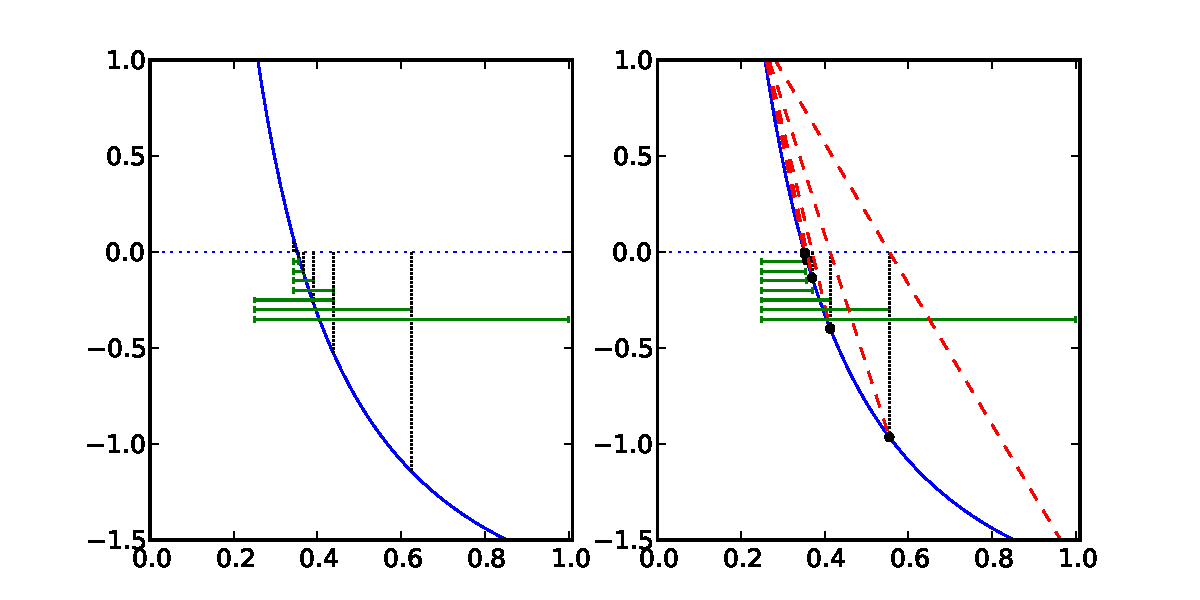
\includegraphics[width=\textwidth]{plots/bisektion}
  \caption{Links: Bisektion für die Funktion $f(r) = e^{-r}/r -
    \phi_0$, hier nur mit $\phi_0=2$, da die genaue Form der Funktion
    für diese Methode unerheblich ist. Blau dargestellt ist wieder
    $f$, die grünen Balken markieren die nacheinander generierten,
    kleiner werdenden Intervalle $[a_n, b_n]$. Die gestrichelten,
    schwarzen Linien markieren die Intervalmitten $m_n$, die im
    nächsten Schritt eine der beiden Intervalgrenzen werden. Rechts:
    Regula falsi für dieselbe Funktion. Die Funktion ist streng
    konvex, daher reagiert die Regula falsi lethargisch und ist der
    Bisektion unterlegen; die Intervalle verkürzen sich praktisch
    nicht mehr, da die untere Anfangsgrenze $1/4$ nie versetzt wird,
    nur die obere Grenze.}
  \label{fig:bisektion}
\end{figure}

\section{\keyword{Regula falsi}}

Sowohl die Bisektion wie auch die Sekantenmethode benötigen zwei
Startwerte. Daher liegt es nahe, die Verfahren zu kombinieren.
Bei der \emph{Regula falsi} wird wie bei der Bisektion ein Interval
$[a,b]$ schrittweise verkleinert so dass dieses stets wenigstens eine
Nullstelle enthält. Anders als bei der Bisektion wird der neue
Randpunkt $m$ allerdings nicht einfach als Intervalmitte bestimmt,
sondern mit Hilfe der Sekantenmethode, mit den beiden
Intervalrandpunkten $a$ und $b$ als Stützstellen:
\begin{equation}
  m = b - f(b)\frac{b - a}{f(b) - f(a)} =
  \frac{f(b)a - f(a)b}{f(b) - f(a)}.
\end{equation}
Da $f(a)f(b)<0$, schneidet die Sekante die Nulllinie immer im
Interval.  Dadurch verkleinert sich das Interval schneller als beim
Bisektionsverfahren, sofern die Nullstelle der Sekante dicht an der
echten Nullstelle liegt. Hat die Funktion im Intervall allerdings
einen Wendepunkt, ist also nicht streng konkav oder konvex, dann wird
die Regula falsi sehr langsam, was auch als Lethargie bezeichnet
wird. Der Grund ist, dass eine der beiden Intervallgrenzen sehr dicht
an die Nullstelle rückt, und im folgenden nur noch diese Grenze
minimal verbessert wird, während die zweite Grenze unverändert
bleibt. Dies ist zum Beispiel in Abbildung~\ref{fig:bisektion} rechts
gezeigt. Leider sind nicht streng konkave oder konvexe Funktionen eher
die Regel als die Ausnahme, daher ist die einfache Bisektion oft
schneller als die Regula falsi.  Die Regula falsi ist nur dann die
schnellste und stabilste Nullstellensuche, falls die Ableitung der
Funktion nicht bekannt ist, man aber weiß, dass die Funktion streng
konvex oder konkav ist.

\section{Newtonverfahren in mehreren Dimensionen}
\index{Newtonverfahren>in mehreren Dimensionen}
\index{Gleichungssysteme>nichtlineare}

Bis jetzt haben wir das Newtonverfahren nur für eindimensionale
Funktionen betrachtet. Im mehrdimensionalen funktioniert das Verfahren
aber sehr ähnlich, wobei die Ableitung zur Jacobimatrix wird.

Sei also $f\in C^1(M, \RR^n)$ eine stetig differenzierbare Abbildung
von $M\in\RR^n$ in den $\RR^n$. Wir suchen nun eine Nullstelle
$\overline{x}\in D$, \dh eine Lösung des nichtlinearen
Gleichungssystems $f(x) = 0$.

Wie schon im Eindimensionalen starten wir mit einer Näherung
$x^{(0)}\in M$, und berechnen die nächste Näherung $x^{(1)}$ durch
Linearisieren von $f$ in $x^{(0)}$. Die Linearisierung ergibt sich aus
der Taylorentwicklung:
\begin{equation}
  \label{eq:linnewton}
  F(x^{(1)}) \,\dot{=}\, F(x^{(0)}) +
  F'(x^{(0)})\left(x^{(1)}-x^{(0)}\right),
\end{equation}
wobei
\begin{equation}
  F'(x) = \left(\frac{d}{dx_j}F_k(x)\right)_{k,j} = 
  \begin{pmatrix}
    \frac{d}{dx_1}F_1(x) & \ldots & \frac{d}{dx_n}F_1(x)\\
    \vdots               &        & \vdots \\
    \frac{d}{dx_1}F_n(x) & \ldots & \frac{d}{dx_n}F_n(x)
  \end{pmatrix}
\end{equation}
die \emph{\keyword{Jacobimatrix}} von $f$ an der Stelle $x$ bezeichnet.
Die neue Näherung $x^{(1)}$ suchen wir als Nullstelle der
Linearisierung \eqref{eq:linnewton}, also aus der Bedingung
$F(x^{(1)})\stackrel{!}{=} 0$. Da wir ja damit nur die
linearisierte Gleichung gelöst haben, linearisieren wir erneut im
neuen Punkt $x^{(1)}$, und so weiter. Ein Schritt des Newtonverfahrens
ist dann also
\begin{equation}
  x^{(m+1)} = x^{(m)} + d^{(m)}\quad\text{mit}\;
  F'(x^{(m)})\,d^{(m)} = -F(x^{(m)}).
\end{equation}
Die \emph{Newtonkorrektur} $d^{(m)}$ wird als aus der Lösung eines
linearen Gleichungssystems gewonnen, zum Beispiel mit Hilfe der
Gaußelimination. Allerdings ist $f'$ im Allgemeinen vollbesetzt, daher
verwendetet man normalerweise schnellere, approximative Verfahren, die
wir später kennenlernen werden. Ist $F'(x^{(m)})$ in einem Schritt
singulär, so bricht das Verfahren ab. Ansonsten wird weiter iteriert,
bis $\norm{d^{(m)}}$ hinreichend klein ist.

Auch im mehrdimensionalen konvergiert dieses Verfahren lokal
mindestens quadratisch, sofern in einer abgeschlossenen Umgebung der
Nullstelle $\norm{F'(x)^{-1}}$ beschränkt ist und $f$ zweifach stetig
differenzierbar. Allerdings gibt es kein langsames Verfahren ähnlich
der Bisektion, dass man dem Vefahren vorausschicken könnte, um die
Nullstelle einzugrenzen. Die globale Suche nach Nullstellen in
mehreren Dimensionen ist also eine schwierige Aufgabe. Eine
Möglichkeit ist, zunächst mit Hilfe von Optimierungsverfahren ein
$x_0$ zu finden mit möglichst kleiner Norm $\norm{f(x_0)}$, und von
dort das (gedämpfte) Newtonverfahren zu starten. Die globale
Optimierung in vielen Dimensionen ist selber eine sehr schwierige
Aufgabe, allerdings existieren hierfür Ansätze wie genetische
Algorithmen oder Simulated Annealing, die wir später kennenlernen
werden.

\subsection{Gedämpftes Newtonverfahren}
\index{Newtonverfahren>gedämpftes}

Leider ist im Mehrdimensionalen die Umgebung um die Nullstelle, in der
das Verfahren konvergiert, oftmals deutlich kleiner. Das Verfahren
springt dann leicht über die Nullstelle hinweg, wie es im
eindimensionalen nur am Anfang des Verfahrens vorkommt
(\zb Abbildung~\ref{fig:newton} rechts, im ersten Schritt). Um dies
zu verhindern, kann man die Schrittweite reduzieren, als den Schritt
$d^{(m)}$ verkürzen. Die Iteration lautet dann
\begin{equation}
  x^{(m+1)} = x^{(m)} + \lambda d^{(m)}\quad\text{mit}\;
  F'(x^{(m)})\,d^{(m)} = -F(x^{(m)}),
\end{equation}
wobei die Dämpfung $\lambda\in (0,1]$ so gewählt wird, dass
$\norm{F(x^{m+1})}\le\norm{F(x^{m})}$. Dazu wird zum Bespiel mit
$\lambda=1$ begonnen, und $\lambda$ solange verringert, bis die
Bedingung erreicht ist.

\begin{lstlisting}[style=floating,deletekeywords={lambda},
caption={Gedämpftes Newtonverfahren in mehreren
Dimensionen. \lstinline!f(x)! muß
eine vektorwertige Funktion sein, \lstinline!fprime(x)! ihre
Ableitung, d.h. eine matrixwertige Funktion.}]
# Gedaempftes Newtonverfahren
#############################

def gedaempfter_newton(f, fprime, x0, epsilon):
   xn = x0
   konvergiert = False
   while not konvergiert:
      # Newton-Korrektur
      dn = solve(fprime(xn), f(xn))
      if norm(dn) < epsilon:
         konvergiert = True
      else:
         # Schrittweitendaempfung
         lambda = 1.0
         abstieg = False
         while not abstieg:
            # neue Naeherung
            xneu = xn + lambda*dn
            if norm(f(xneu)) < norm(f(xn)):
               abstieg = True
            else:
               lambda = lambda / 2.0
         xn = xneu
   return xn
\end{lstlisting}

%%% Local Variables: 
%%% mode: latex
%%% TeX-master: "padc"
%%% TeX-PDF-mode: t
%%% End: 


\printbibliography

\printindex

\end{document}

%%% Local Variables: 
%%% mode: latex
%%% TeX-master: t
%%% TeX-PDF-mode: t
%%% End: 
